\documentclass[12pt,a4paper,oneside]{report}            % Single-side
%\documentclass[11pt,a4paper,twoside,openright]{report} % Duplex

% Document classes
% article - For articles in scientific journals, presentations, short reports, program documentation, invitations, ...
% report - For longer reports containing several chapters, small books, thesis, ...
% book - For real books.
% beamer - For writing presentations (see https://en.wikibooks.org/wiki/LaTeX/Presentations)

% Document Class Options
% 10pt, 11pt, 12pt - If no option is specified, 10pt is assumed.
% a4paper, letterpaper,... - a5paper, b5paper, executivepaper, and legalpaper can be specified.
% fleqn - Typesets displayed formulas left-aligned instead of centered.
% leqno - Places the numbering of formulas on the left hand side instead of the right.
% titlepage, notitlepage - Specifies whether a new page should be started after the document title or not.
% twocolumn - Instructs LaTeX to typeset the document in two columns instead of one.
% twoside, oneside - Specifies whether double or single sided output should be generated.
% landscape - Changes the layout of the document to print in landscape mode.
% openright, openany - Makes chapters begin either only on right hand pages or on the next page available. This does not work with the article class, as it does not know about chapters.

% set the main variables
\newcommand{\authorFamilyName}{Deák}
\newcommand{\authorFirstName}{Elemér Dávid}

\newcommand{\consultantATitle}{Dr.~}
\newcommand{\consultantAFamilyName}{Plesz}
\newcommand{\consultantAFirstName}{Balázs}

\newcommand{\consultantBTitle}{Dr.~}
\newcommand{\consultantBFamilyName}{Szabó}
\newcommand{\consultantBFirstName}{Péter Gábor}

% Document's title
\newcommand{\documentTitle}{MEMS rezgőkondenzátor\\ tervezése és modellezése} % Document's title
\newcommand{\documentTitleMeta}{MEMS rezgőkondenzátor tervezése és modellezése} % Title used as pdf metadata
\newcommand{\department}{\bmeeet}                                               % Department
\newcommand{\documentDegree}{\msc}                                              % Education degree \bsc or \msc
\newcommand{\documentType}{diplomatervet}                                       % Word to insert in the student statement szakdolgozatot or diplomatervet

% Used packages
\usepackage[utf8]{inputenc}                                                     % Accept different input encodings
\usepackage{geometry}                                                           % Flexible and complete interface to document dimensions
\usepackage{physics}                                                            % Physical symbols like div, rot
\usepackage{amsfonts,amsmath,amssymb}                                           % Mathematical symbols.
\usepackage{textcomp, gensymb}                                                  % Generic symbols for both text and math mode
\usepackage[uline]{hhtensor}                                                    % Matrix and vector sign
\usepackage[magyar]{babel}                                                      % Multilingual support for Plain TEX or LATEX
\usepackage{t1enc}

\usepackage{graphicx}                                                           % Enhanced support for graphics
\usepackage{booktabs}                                                           % Publication quality tables in LATEX
\usepackage{setspace}                                                           % For setting line spacing
\usepackage{color}                                                              % red, green, blue, yellow, cyan, magenta, black, white

\usepackage[backend=biber,style=numeric,sorting=none,maxbibnames=99]{biblatex}  % Using biblatex
\BiblatexHungarianWarningOff
\addbibresource{bib/mybib.bib}                                                  % Bibliography source file

\usepackage{csquotes}
\usepackage{pdfpages}                                                           % Include PDF documents in LATEX
\usepackage[unicode,pdfpagelabels,hyperindex,hyperfigures]{hyperref}            % For hyperlinks in the generated document.
\usepackage{listings}                                                           % For code insertion
\usepackage{caption}                                                            % For caption menagement
\usepackage{subcaption}                                                         % For subfigure captions
\usepackage{float}                                                              % For floating figures

\usepackage{array}                                                              % For tables with fixed cell size

\widowpenalty=10000                                                             % Extra penalty for breaking before last line of a paragraph
\clubpenalty=10000                                                              % Extra penalty for breaking after first line of a paragraph
\def\hyph{-\penalty0\hskip0pt\relax}                                            % Enable hyphenation for words including a hyphen
\displaywidowpenalty=10000                                                      % Extra penalty for breaking before last line before a display math
\interfootnotelinepenalty=10000                                                 % Extra value for interline penalty in footnotes
\sloppy                                                                         % Makes TeX obey margins by stretching inter word spaces

\newenvironment{nohyphens}{                                                     % disable hyphens for a paragraph
  \par
  \hyphenpenalty=10000
  \exhyphenpenalty=10000
  \sloppy                                                                       % Makes TeX obey margins by stretching inter word spaces
}{\par}

\setcounter{biburllcpenalty}{100}                                               % Enable URL breaks at lowercase letters
\setcounter{biburlucpenalty}{100}                                               % Enable URL breaks at uppercase letters

\usepackage{titlesec}                                                           % Setting the chapter's style
                                                        % Main includes
\newcommand{\bme}{Budapesti Műszaki és Gazdaságtudományi Egyetem}
\newcommand{\vik}{Villamosmérnöki és Informatikai Kar}

\newcommand{\bmeeet}{Elektronikus Eszközök Tanszéke}

\newcommand{\madeBy}{Készítette}
\newcommand{\consultant}{Konzulens(ek)}

\newcommand{\bsc}{Szakdolgozat}
\newcommand{\msc}{Diplomaterv}
\newcommand{\tdk}{TDK dolgozat}
\newcommand{\bsconlab}{BSc Önálló laboratórium}
\newcommand{\msconlabi}{MSc Önálló laboratórium 1.}
\newcommand{\msconlabii}{MSc Önálló laboratórium 2.}
\newcommand{\mscdiptervi}{MSc Diplomatervezés 1.}
\newcommand{\mscdiptervii}{MSc Diplomatervezés 2.}

\newcommand{\introductionText}{Bevezetés}
\newcommand{\thankYouText}{Köszönetnyilvánítás}
\newcommand{\appendixText}{Függelék}

\def\lstlistingname{lista}

\newcommand{\documentAuthor}{\authorFamilyName{} \authorFirstName}
\newcommand{\authorMeta}{\documentAuthor}
\newcommand{\consultantA}{\consultantATitle\consultantAFamilyName{} \consultantAFirstName}
\newcommand{\consultantB}{\consultantBTitle\consultantBFamilyName{} \consultantBFirstName}

\newcommand{\appendixnumber}{6}                                                 % Appendix start with the 6th letter of the alphabet (F)

% Equations with reference label
\newcommand{\equref}[2]{
    \begin{equation}\label{#2}
        #1
    \end{equation}
}

% Include grpahics in classic mode (pdf, jpg, png), ratio based
\newcommand{\imgsrc}[4]{
    \begin{figure}[H]
        \centering
        \resizebox{#4\linewidth}{!}{\includegraphics{#1}}
        \captionsetup{width=.85\linewidth, aboveskip=10pt, justification=centering}
        \caption{#2}
        \label{#3}
    \end{figure}
}

% Include two figures side by side
\newcommand{\imgsrclr}[8]{
    \begin{figure}[H]
        \centering

        % images
        \begin{minipage}{.5\textwidth}
            \centering
            \resizebox{#7\textwidth}{!}{\includegraphics{#1}}
        \end{minipage}%
        \begin{minipage}{.5\textwidth}
            \centering
            \resizebox{#8\textwidth}{!}{\includegraphics{#2}}
        \end{minipage}

        % captions
        \begin{minipage}[t]{.5\textwidth}
            \captionsetup{width=.85\linewidth, aboveskip=10pt, justification=centering}
            \caption{#3}
            \label{#5}
        \end{minipage}%
        \begin{minipage}[t]{.5\textwidth}
            \captionsetup{width=.85\linewidth, aboveskip=10pt, justification=centering}
            \caption{#4}
            \label{#6}
        \end{minipage}
    \end{figure}
}

% Increase tables' linespace
\renewcommand{\arraystretch}{1.2}

% setting the margins
\geometry{top=25mm,bottom=25mm,left=35mm,right=25mm}                           % geometry for printing
% \geometry{top=25mm,bottom=25mm,left=25mm,right=25mm}                            % geometry for online pdf

% setting line spacing
\renewcommand{\baselinestretch}{1.25}

\author{\documentAuthor}
\title{\documentTitle}

\renewcommand{\captionlabelfont}{\bf}

% Setup hyperref package
\hypersetup{
    unicode=true,                                                               % non-Latin characters in Acrobat's bookmarks
    pdftitle={\documentTitleMeta},                                              % title
    pdfauthor={\authorMeta},                                                    % author
    pdfsubject={\documentType},                                                 % subject of the document
    pdfcreator={\authorMeta},                                                   % creator of the document
    pdfproducer={},                                                             % producer of the document
    pdfkeywords={},                                                             % list of keywords (separate then by comma)
    pdfnewwindow=true,                                                          % links in new window
    colorlinks=true,                                                            % false: boxed links; true: colored links
    linkcolor=black,                                                            % color of internal links
    citecolor=black,                                                            % color of links to bibliography
    filecolor=black,                                                            % color of file links
    urlcolor=black                                                              % color of external links
}


\begin{document}

% setting the chapter format
\titleformat{\chapter}[hang]{\Huge\bfseries}{\thechapter\hspace{10pt}{|}\hspace{10pt}}{0pt}{\Huge\bfseries}
\titlespacing*{\chapter}{0pt}{-40pt}{20pt}

% turn off page numbering
\pagenumbering{gobble}
\hypersetup{pageanchor=false}

\begin{titlepage}
\begin{center}

\includegraphics[width=60mm,keepaspectratio]{figures/bme_logo.pdf}\\
\vspace{0.3cm}
\textbf{\bme}\\
\textmd{\vik}\\
[5cm]

\vspace{0.4cm}
{\huge \bfseries \documentTitle}\\[0.8cm]
\vspace{0.5cm}
\textsc{\Large \documentDegree}\\[4cm]

{
	\renewcommand{\arraystretch}{0.85}
	\begin{tabular}{cc}
	 \makebox[7cm]{\emph{\madeBy}} & \makebox[7cm]{\emph{\consultant}} \\ \noalign{\smallskip}
	 \makebox[7cm]{\documentAuthor} & \makebox[7cm]{\consultantA} \\
	  & \makebox[7cm]{\consultantB} \\
	\end{tabular}
}

\vfill

\includegraphics[width=40mm,keepaspectratio]{figures/eetlogo.png}\\
\textbf{\department}\\
{\large \today}
\end{center}
\thispagestyle{empty}
\end{titlepage}
                                                     % Titlepage
\tableofcontents\vfill                                                          % Table of Contents

% turn off page numbering
\pagenumbering{gobble}

\begin{center}
\large
\textbf{HALLGATÓI NYILATKOZAT}\\
\end{center}

Alulírott \emph{\authorMeta}, szigorló hallgató kijelentem, hogy ezt a \documentType{} meg nem engedett segítség nélkül, saját magam készítettem, csak a megadott forrásokat (szakirodalom, eszközök stb.) használtam fel. Minden olyan részt, melyet szó szerint, vagy azonos értelemben, de átfogalmazva más forrásból átvettem, egyértelműen, a forrás megadásával megjelöltem.

Hozzájárulok, hogy a jelen munkám alapadatait (szerző(k), cím, angol és magyar nyelvű tartalmi kivonat, készítés éve, konzulens(ek) neve) a BME VIK nyilvánosan hozzáférhető elektronikus formában, a munka teljes szövegét pedig az egyetem belső hálózatán keresztül (vagy autentikált felhasználók számára) közzétegye. Kijelentem, hogy a benyújtott munka és annak elektronikus verziója megegyezik. Dékáni engedéllyel titkosított diplomatervek esetén a dolgozat szövege csak 3 év eltelte után válik hozzáférhetővé.

\begin{flushleft}
\vspace*{1cm}
Budapest, \today
\end{flushleft}

\begin{flushright}
 \vspace*{1cm}
 \makebox[7cm]{\rule{6cm}{.4pt}}\\
 \makebox[7cm]{\emph{\documentAuthor}}\\
 \makebox[7cm]{hallgató}
\end{flushright}
\thispagestyle{empty}

\vfill
% \clearpage
\thispagestyle{empty} % an empty page

\hypersetup{pageanchor=true}
                                                   % Declaration

\pagenumbering{arabic}                                                          % Turn on arabic page numbering
\setcounter{page}{1}

\chapter*{Kivonat}\addcontentsline{toc}{chapter}{Kivonat}

Dolgozatomban bemutatok egy Kelvin-szondás mérésre alkalmas mikroelektromechanikai rendszer (MEMS) tervezési folyamatát. A Kelvin-mérés során a mintafelület elektrosztatikus potenciálviszonyait tudjuk vizsgálni, a mintával történő kontaktálás nélkül, így nem megzavarva annak felületi viszonyait. A Kelvin-mérés a félvezetőiparban egy elterjedt és jól ismert mérési metódus, mely remekül használható kutatási célokra.

A tervezés első fázisaiban a szükséges paraméterek megállapítása volt a cél, így elektromágneses szimulációkat végeztem, melyek segítségével specifikálható a tervezendő MEMS eszköz mechanikai szerkezete. Az elektromágneses szimulációkat a felületelem módszer felhasználásával végeztem el, így elkerülve a térfogati diszkretizációt és csökkentve a szükséges számítási kapacitás mértékét. A szimulálandó modelltér méretének meghatározásához egy analitikai modellt dolgoztam ki, mely a kialakuló elektromágneses mezőt megfelelően közelíti. A mező jellegének javítása érdekében egy fókuszálási módszert is hozzáadtam a mérőfejhez. A szimulációk eredményéül előálló elektromágneses tér alapján definiáltam a mérőfej érzékenységét és meghatároztam annak térbeli eloszlását. A szimulációk során előálló elosztott paraméterű modell alapján egy koncentrált paraméterű helyettesítőképet alkottam, melyet a későbbi számítások során fel is használtam. A Kelvin-szondás mérés kimeneti jeléül szolgáló jeleket a koncentrált paraméterű modell alapján közelítettem, mely a mechanikai specifikáció megalkotását tette lehetővé. A szimulációs és adatfeldolgozó munkafolyamatot MATLAB és PYTHON scriptek segítségével automatizáltam, kihasználva a COMSOL MULTIPHYSICS adta lehetőségeket. A szimulációk és utófeldolgozáshoz szükséges idő ezáltal jelentős mértékben csökkenthető volt.

Az elektromágneses térszámítás eredményeinek birtokában elkezdtem a mechanikai szerkezet méretezését és tervezését. A Kelvin-szondás méréshez szükséges rezgést termomechanikus csatolás lévén érem el, elkerülve az elektrosztatikus gerjesztés okozta interferenciát. A működési sebesség növelése érdekében a gerjesztést pár tíz-száz kHz frekvencián kell elvégezni, mely megfelelő méretezés mellett megegyezik a rendszer mechanikai rezonanciájával, ezáltal növelve a kitérés amplitúdóját. A szükséges számítási igény csökkentése érdekében tranziens szimulációt csak a mérőfej validációjára használtam, a méretezés során csak szinuszos állandósult állapotot vizsgáltam. Szükséges volt továbbá a termomechanikus, csatolt egyenletek szinuszos állandósult állapotbeli alakjának implementációja a szimulációs szoftverben. A mechanikai gerjesztést végző termikus beavatkozást optimalizáltam a nagyobb kitérések érdekében, valamint megvizsgáltam a lehetséges csillapítási mechanizmusokat.

A mérőfej tervezésének utolsó lépéseként megvizsgáltam a mérőfej gyárthatóságának feltételeit, annak CMOS kompatibilitását és elkészítettem egy kezdetleges tesztstruktúra tervét mellyel a termikus beavatkozó teljesítménye mérhető.

\chapter*{Abstract}\addcontentsline{toc}{chapter}{Abstract}

In my thesis I present the design process of a microelectromechanical system (MEMS) which is capable of performing a Kelvin probe measurement. During the measurement we probe the electrostatic potential of a sample without making conductive contact to it, therefore not disturbing its surface state. The Kelvin measurement is a widely known and accepted methodology in the semiconductor industry which is well suited for research purposes.

In the first phase of development my goals was to specify the necessary parameters, so first I simulated the electromagnetic (EM) field which made the specification of the mechanical structure of the MEMS device possible. I ran the EM simulations using the Boundary Element Method (BEM). Thanks to this, I avoided the need for three dimensional discretisation which in return reduced the required computing power. To estimate the size of the model space required to simulate I derived an analytical model, which approximated the resulting EM field. To optimize the EM field I added a focusing method to the probe's setup. From these simulations I defined the sensitivity of the probe and determined its spatial distribution. Using the distributed simulations I made a lumped element model to replace the original, which I used for further numerical calculations. The output signals of the Kelvin probe measurement was approximated using this lumped model, which made the specification of the mechanical model possible. The simulational and post processing workflow were automated by MATLAB and PYTHON scripts. These scripts utilized the built-in features of COMSOL MULTIPHYSICS that greatly reduced the time needed for the simulations and post processing.

Following the results of the EM field calculations I began designing the mechanical construction. The necessary vibration for the Kelvin probe is generated by a thermomechanical coupling in which way we avoid the interference caused by the usual electrostatic excitation. To increase the operating speed, the excitation is done in the tens to hundreds of kilohertz range, which in a well designed case is the same as one of the resonant frequencies of the probe therefore increasing the resulting amplitude of the vibration. To decrease the necessary computational power I only ran transient simulations to verify the probe, while for the design part I used a sinusoidal steady-state. To utilize the sinusoidal steady-state solver it was necessary to derive these versions of the coupled thermomechanical equations and to implement these in the software as well. The thermal excitation, which drives the mechanical system, was optimized for the greater amplitudes. I also examined the effect of a possible dissipation mechanism too.

The final stage of the design process was to examine the manufacturability, the CMOS compatibility of the designed Kelvin probe and to design a rudimentary test structure, which is capable of measuring the thermal actuator's performance.

\vfill
                                                      % Abstract
\chapter{Bevezető}

A mikroelektronikai méréstechnika és anyagtudomány egy igen fontos mérési módszere a Kelvin-szondás felületi potenciál mérés\cite{Kelvin_desc}, amely a gyártás- és vizsgálattechnológiai ágazatokban számos helyen fellelhető, így a módszer fejlesztése is fontos feladat. Egy lehetséges módszer, az áramkörök méretének csökkenésével analóg módon, a vizsgáló berendezések méretének csökkentése kihasználva a mikroelektromechanikai rendszerek (MEMS) által biztosított pontos és gyors működést. A mérőrendszer fejlesztése során egy újszerű meghajtási móddal kísérleteztem, a rezonanciafrekvencián történő mechanikai deformáció hőtáguláson alapuló megvalósításával.

MEMS-eknél nagy kitérések elérésére általában nagy méretű, meanderezett rugókat és beavatkozókat tartalmazó eszközöket használnak\cite{micromirror}\cite{large_out_of_plane}. Ezen eszközök hátránya azonban a relatíve nagy méret és az ezzel együtt járó viszonylag nagy tömeg, mely korlátozza a rendszer rezonanciafrekvenciáját és ezzel együtt a mérési sebességet. Egy másik út, a meanderes struktúrákkal szemben, a hosszú egyenes konzolokkal rendelkező struktúrák, melyek képesek jelentős kitéréseket produkálni\cite{brai}, ám a méretükből és tömegükből származó korlátok ezeket a struktúrákat is érintik. Dolgozatomban egy rövid karokkal és kis felülettel rendelkező MEMS struktúrát mutatok be, amely így mentesül az előbb említett hátrányoktól, azonban így a $\mu m$-es kilengések elérése nagyobb kihívás.

Diplomatervemben folytatom és továbbfejlesztem korábbi munkáim\cite{bsc}\cite{tdk2020} során szerzett tudást és ismereteket. Az itt bemutatott MEMS eszköz immár a harmadik változata annak a Kelvin-szondás méréshez készített mérőfejnek, melyet szeretnénk megvalósítani. Az első változatban\cite{bsc} egy torziós elven működő rugót és egy elektrosztatikus beavatkozót szerettem volna felhasználni a MEMS eszköz kitérítésére, azonban a tervezett konstrukció nem volt képes elegendően nagy kitéréseket produkálni, valamint nem a teljes működési tartományon volt stabil\cite{bsc_instability}. A második változathoz\cite{tdk2020} lecseréltem az elektrosztatikus meghajtást egy termomechanikusra, így elkerülve az elektrosztatikus meghajtásból adódó zavarokat. Ez a változat egy meanderes rugóval volt ellátva, valamint egy viszonylag nagy mérőfelülettel rendelkezett, így a működési frekvenciatartománya nem volt elegendően nagy.

A tervezett mérőfej bemutatása előtt azonban a munkám megértéséhez elengedhetetlen ismeretek átadásával kezdem a dolgozatomat, melyben először is áttekintem a Kelvin-szondás mérés módszertanát és ismertetem a szükséges fogalmakat és mennyiségeket. A MEMS mérőfej méretezéséhez egy elektromágneses és egy termomechanikus modellt állítok fel a geometriai paraméterek tervezéséhez. A diplomatervemben bemutatásra kerülnek a szükséges matematikai modellek és fogalmak, valamint a mérőfej számítógépes modelljei, a rajtuk végzett szimulációk és azok eredményei. A mérőfej megtervezése után kitérek a gyártástechnológiai megvalósíthatóság kérdésére is, valamint egy kezdetleges tesztstruktúrát is megadok, melyen a termomechanikus kitérést lehet tesztelni és mérni.
                                                  % Main content
\chapter{Mérési eljárás}

\section{Kontakt potenciál kialakulása}
\label{contact}

A dolgozat témáját adó Kelvin-szondás mérés megértéséhez először szeretném tisztázni a mérés tárgyát adó fizikai jelenséget, a felületi kontakt potenciált és annak kialakulását. Két különböző anyagi minőséggel rendelkező szilárdtest fémes kapcsolatba hozásánál, az eltérő energetikai sávszerkezet miatt, a kontaktus felületén egy kiegyenlítődési folyamat indul meg, melyet a kilépési munkával jellemezhetünk. A szilárdtest kilépési munkája (angolul work function-je) alatt azt a termodinamikai energiamennyiséget értjük, mely egy a szilártesten belüli elektron eltávolításához szükséges.

\equref{dE = \mu\ dN}{eqn:chemical_pot}

\Aref{eqn:chemical_pot}. egyenletben E az energia, $\mu$ a kémiai potenciál és dN a részecskeszám változás. Ez az energia nem tartalmazza az elektron további erőterekből való eltávolítását - ilyen például az elektrosztatikus tér - így csak a kristályráccsal való kölcsönhatását szüntetjük meg. A kiszakított elektronok energiaszintjét definiáljuk vákuum szintnek és a további energiaszinteket ettől az energiaértéktől tudjuk mérni. Ezt felhasználva definiálhatjuk a kilépési munkát, ami a kémiai potenciál és vákuum szint energiakülönbsége.

\equref{W_f = E_\text{vákuum}-\mu}{}

A kémiai potenciál azzal az energiamennyiséggel egyezik meg, mellyel a szilárdtest összes termodinamikai energiája megváltozik, ha egy elektront hozzáadunk, vagy elveszünk a szilárdtestből, ahogy az \aref{eqn:chemical_pot}. egyenletből látszik is. A kilépési munka nem csak az anyagi minőség függvénye, hanem a tömbi anyag felületi viszonyaié is. Ilyenek lehetnek például a kötött töltések, lógó kötések, valamint a szennyező atomok jelenléte. Ez a kölcsönhatás teszi lehetővé, hogy a kilépési munka mérésével az anyag felületi viszonyairól is képet kapjunk.

A kontaktus határfelületén a kisebb kilépési munkával rendelkező, tehát átlagosan nagyobb potenciális energiájú elektronok, az energetikailag kedvezőbb alacsonyabb energiájú állapot felé áramlanak a diffúziónak köszönhetően. A termikus mozgás következtében az elektronok el tudnak jutni a kontaktus másik oldalára és ott be tudják tölteni az alacsonyabb energiaszinteket, így ezen a térrészen a nagyobb energiájú elektronok koncentrációja lecsökken. Ez a koncentrációkülönbség hajtja tovább a diffúziót a termikus mozgásnak köszönhetően. Ennek következtében a határfelület mentén egy töltött kettősréteg alakul ki. A kisebb kilépési munkájú anyagban a hiányzó elektronok lokalizált pozitív atomtörzseket hagynak hátra, míg a nagyobb kilépési munkájú térrészben lévő elektron többlet negatív tértöltésként jelentkezik. Ez a folyamat addig tart, míg a kialakuló töltés kettősréteg - vagy más szóval kiürített réteg - elektromos potenciálja nem kompenzálja a két térrész energiaszintjei közötti különbségét.\cite{mizsei} A folyamatot jól szemléltetik \aref{fig:contact_potential_1}. és \aref{fig:contact_potential_2}. ábrák, melyen két eltérő fém sávszerkezetét valamint az egymáshoz viszonyított kontakt potenciáljukat ábrázoltam. Az ábrán E = 0 a vákuum szintet jelöli, $e\phi_1$ és $e\phi_2$ a két fém kilépési munkáit, ahol e az elektromos töltés egysége és $\xi$ a kialakuló elektromos teret.

\imgsrclr{figures/Kelvin/initial_energy.png}{figures/Kelvin/equilibrium_energy.png}{Kiindulási energiaszerkezet}{Egyensúlyi energiaszerkezet}{fig:contact_potential_1}{fig:contact_potential_2}{1}{1}

A töltés kettősréteg térbeli változása leírható egy Poisson-Boltzmann-egyenlettel, hiszen a kilépési munkák és a töltéshordozók koncentrációja összefügg\cite{Garrett_Brattain}. Az egyenlet megoldásából jól látható\cite{poisson-boltzmann}, hogy a tértöltésréteg vastagsága a határfelülettől mérve függ az anyag dielektromos állandójától, valamint a mozgóképes töltéshordozók koncentrációjától. Fémek esetében a tértöltésréteg néhány atomsorig tart, így az ott kialakuló sávelhajlás elhanyagolható és a töltéssűrűség egy megfelelő Dirac-deltával közelíthető. Félvezetők esetében a kiürített réteg vastagsága elsősorban az adalékolástól függ és akár a $\mu$m-t is elérheti. Ennek következtében kis geometriai méretek esetén a felületi jellemzők nagymértékben befolyásolják a félvezető elektromos tulajdonságait.\cite{mizsei} Ez a folyamat felelős például a MOS tranzisztorok rövidcsatornás hatásainak egy részéért is, a Source és Drain elektródáknál lévő sávelhajlások egymásra lapolódásából fakadóan\cite{poisson-boltzmann}.

Azt a mélységet, amelyen belül a külső elektromos tér hatása még érzékelhető a szilárdtestek kategorizálására is használhatjuk. A fémek esetében a külső elektromos tér néhány atomi távolságig fejti ki hatását, így jó közelítéssel állíthatjuk, hogy az elektromos tér a fémekbe nem hatol be, és a fémek belsejében azonosan nulla. Szigetelők esetében viszont, az elektromos tér a szigetelő belsejében lévő dipólusokra forgatónyomatékot fejt ki, így polarizálva azokat. Ennek következtében a szigetelő belsejében egy elektromos tér alakul ki, vagyis a külső tér a szigetelő teljes térfogatában kifejti hatását. A fémekkel és a szigetelőkkel ellentétben a félvezetőknél a külső elektromos tér hatása az előbb említett két eset között helyezkedik el, vagyis az adalékolástól függően változik a külső elektromos tér befolyásának mértéke. Ugyanakkor a geometriai méretek csökkenésével a félvezetők egyre inkább szigetelőként kezdenek viselkedni, a fogalom ezen értelmében, vagyis a külső elektromos tér hatását nem árnyékolják le.

Az eddigi ábrákon lévő energiaskála az elektronok termodinamikai energiáit tartalmazta, ugyanakkor kihagyta az elektrosztatikus kölcsönhatásból származó potenciális energiát. A kiegyenlítődési folyamatok jobb megértése érdekében a sávdiagramokon az energiákhoz hozzáadjuk az elektrosztatikus potenciálból származó járulékokat is. Ezzel a járulékkal kiegészített energiaskálát elektrokémiai potenciálnak nevezzük. Ennek a potenciálnak a használatával láthatóvá válik a termodinamikai egyensúly kialakulása, hiszen a két anyagban az elektrokémiai potenciálok azonos energiaszintre kerülnek termikus egyensúlyban. \ref{fig:electrochemical_potential}. ábra. Az elektrokémiai potenciál alkalmazásának hátránya, hogy a vákuum szint értéke nem lesz homogén, ahogy az az ábrán is látható.

\imgsrc{figures/Kelvin/electrochemical_potential.png}{Egyensúlyi állapot elektrokémiai potenciállal ábrázolva}{fig:electrochemical_potential}{0.5}

\equref{\phi_{kontakt} = \phi_1 - \phi_2 = \frac{W_{ki1}-W_{ki2}}{e}}{}

Az egyenletben $\phi_1$ és $\phi_2$ a két térrész mellett mérhető elektrosztatikus potenciál, $W_{ki1} W_{ki2}$ az anyagok kilépési munkái és e az elektromos töltés egysége. Az ábrán jól látható, hogy a kontaktus határfelülete mentén egy elektrosztatikus potenciálugrás alakul ki, ez az úgynevezett kontakt potenciál, melynek értéke a két fém kilépési munkáinak különbségéből fejezhető ki. Ennek a potenciálnak a felületi feltérképezésével láthatóvá válnak a vizsgált felületen a különböző adalékolású területek, valamint a tömbi anyag felületi állapotainak hatása is.\cite{surface_states} Ha ismerjük a felület adalékolásának eloszlását, valamint a felületi állapotok lokalizált hatásait akkor készíthetünk ezekből egy felületi eloszlástérképet, mellyel az adott felületi réteg minősítését végezhetjük el. Ilyen minősítő jelzők lehetnek az adaléksűrűség eloszlás, a maszkolás pontossága vagy a felületi szennyeződések darabszáma. Ebből is látszik, hogy a felületi potenciál feltérképezése rendkívül hasznos információt tud szolgálni.

A kontakt potenciálok létrejötte azonban azok mérését is nehezíti, hiszen ez a potenciál nem mérhető szokványos fémes kontaktusokon alapuló potenciálmérési módszerekkel. A jelenség oka, hogy a fémes kontaktus létrejöttekor a kialakuló potenciálugrások a mérőműszer és a minta felülete között pontosan kiegyenlítik a mérendő potenciált, így a teljes rendszer termodinamikai egyensúlyba kerül. Amíg ez az egyensúly nem áll be, addig a szilárdtesten belül létezik egy energiakülönbség, mely tovább tudja hajtani a diffúziót a kiegyenlítődés állapota felé.

\section{Kelvin-szondás mérés}

Az elektrosztatikus potenciál mérésére kézenfekvő egy kapacitív csatolás alkalmazása, ahol a minta felületéhez közel elhelyezett mérő elektróda és a minta felülete között az elektrosztatikus tér teremt kapcsolatot. A mérőfej és a minta közötti csatoló kapacitás pontos ismeretében elviekben számítható lenne a vizsgált felületi potenciál pontos értéke, azonban a mérési szórások ezt a mérési elvet igencsak megbízhatatlanná teszik. A vizsgálati módszer pontosabbá tételére egy lehetséges megoldás a mérést befolyásoló mennyiségek időbeli változtatása, valamint egy közvetett mennyiség mérése, mely a változó paraméterek mellett is konstans tud lenni kiegyenlített esetben. A gyakorlatban ez az időbeli változás a mérőfej-minta távolságának változtatása, melynek következtében a csatoló kapacitás értéke is változik. Az időben változó kapacitás következtében, állandó feszültség mellett, a kondenzátor töltése változik az idő függvényében, ezeket a töltéseket a kondenzátort töltő áram biztosítja. Ha a mérőelektróda potenciálját a vizsgált felület potenciáljával azonosra állítjuk be, úgy a csatoló kondenzátor kapcsain 0 V feszültség keletkezik, így a változó kapacitás mellett is nulla töltés halmozódik fel az elektródán, tehát a töltőáram is nullává válik. Ezen nullaátmenet detektálása teszi lehetővé a felületi potenciál érintésmentes mérését.

A mérőelektróda mintától vett távolságát tetszőleges módon változtathatjuk, azonban ha a távolságot egy adott frekvenciájú periodikus jel szerint változtatjuk, úgy a kialakuló áramjel csak az adott frekvenciát és annak felharmonikusait fogja tartalmazni az időfüggő kapacitás miatt. A legkézenfekvőbb periodikus gerjesztés a harmonikus függvények használata. Mivel a gerjesztés frekvenciája a mérés során ismert, így a mérendő jelben ismertek a mérésből származó információt hordozó frekvenciakomponensek, így ezekre a frekvenciákra jobban illesztett feldolgozó áramkörök és jelfeldolgozás készíthető. A mérési eljárás sematikus felépítését  \aref{fig:measurement_sketch}. ábrán látható.

\imgsrc{figures/Kelvin/measurement_sketch.png}{Kelvin-szondás mérés sematikus összeállítása.}{fig:measurement_sketch}{0.5}

Az ábrán a minta felületi potenciálját az ismeretlen  $\phi_{\text{mérő}}$ értékű feszültségforrás reprezentálja, míg a mérendő potenciált a $\phi_{ismeretlen}$ értékű feszültségforrás. A mérés során a mérőelektróda és a mérendő felület közötti távolságot szinuszosan változtatjuk és mérjük az áramkörben folyó áramot. Az adott elrendezésben ennek következtében a változó kapacitású kondenzátor árama is változik. Az áram mérésére annak megzavarása nélkül csak szűkös elektronikai megvalósítások állnak rendelkezésre, hiszen itt egy átfolyó áramot kell mérnünk a potenciálok megváltoztatása nélkül. Erre egy lehetőség integrált áramköri technológiákkal a mágneses csatoláson alapuló mérés\cite{CMOS_I_measure}, azonban az mérés érzékenysége ($1\mu A/A$) az általunk használt töltőáramokkal ($nA-\mu A$) mérhetetlenül kicsin áramokat eredményezne. Ha eltekintünk a potenciálok meg nem változtatásától, akkor az átfolyó áramokat egy sönt ellenállással át tudjuk konvertálni feszültségé. Ezen feszültségek könnyen mérhetőek számos kapcsolástechnikával a söntön átfolyó áram megzavarása nélkül. Az így beiktatott sönt azonban szétválasztja a mérőelektróda potenciálját a táphoz képest, így a mérési kapcsolást ki kell egészíteni egy potenciál ($\phi$) méréssel is. A sönt ellenállás miatt a mérőfej érzékenyebb lesz a parazita kapacitásokra is, így a vizsgálatok során azokat is figyelembe kell venni.

\chapter{Kelvin-szondás mérőfej tervezése}

A Kelvin mérés megvalósításához egy változtatható kapacitás megvalósítása a cél. A kapacitás egyik fegyverzete a vizsgáló minta felülete, míg másik fegyverzetéül egy mozgatott elektróda szolgálhat. Az elektróda alakja és mérete nagymértékben meghatározza a mérőfej által vizsgált terület méretét. Minél kisebb az elektródánk, annál kisebb az interakciós térrész melyből az információ származik, valamint annál kisebbek a jelintenzitások, hiszen a kapacitás arányos a térrész térfogatával is \aref{eqn:cap_volume}. egyenletnek megfelelően.

\equref{C = \frac{2\int_\Omega \vec{E}\cdot \vec{D} d\Omega}{U^2}}{eqn:cap_volume}

Az egyenletben az integrállal meghatározzuk az $\Omega$ térrészben lévő elektrosztatikus energia mértékét az $\vec{E}$ és $\vec{D}$ vektorokkal, majd elosztjuk a teret létrehozó feszültség négyzetével. Az interakciós térrész csökkentésével növelhető a mérőfej felbontóképessége, hiszen vizsgált jelet csak egy szűkebb felülettel kölcsönhatva veszünk.

Ezt az elvet felhasználva a mérőfej méretét nanométeres nagyságrendbe lehetett szűkíteni\cite{KPFM_1}. Ezen nagy felbontás eléréséhez szükséges a felületi topográfia feltérképezése is, ezt a mérőfej úgynevezett kopogtató üzemmódjával érik el. A mérőfej mintától mért távolságát addig csökkentik míg az a minta felületéhez nem érintkezik. A topográfiai információ begyűjtése után a mérőtűt a minta felett kis távolságban (10-100 nm) rezgetve végzik el a mérést. Ezen kis távolságok esetén a mérőtű mozgatását a mérőtűt gerjesztő AC feszültségjel és az elektrosztatikus vonzást felhasználva valósítják meg. A mérőtű mozgatására egy másik lehetőség a piezoelektromos meghajtás\cite{KPFM_2}, mely során a mérőtűt tartó konzolt egy piezoelektromos beavatkozóval rezgetik a konzol rezonanciafrekvenciáján.

Ezekkel a módszerekkel akár az 1 nm-es felbontás is elérhető, azonban a mérések a több órás nagyságrendbe is eshetnek\cite{KPFM_2}. A mérési idő csökkentése érdekében a laterális felbontóképességet kell csökkentenünk, vagyis növelnünk kell a mérőfej méretét. A mérés sebességét az is gyorsítja, ha a felületről nem szükséges topográfiai információ gyűjtése, hogy a mérőfej ne ütközzön bele a mintába. Ez elérhető, ha a mérőfejet a mintától néhány 10 $\mu m$-es távolságban rezgetjük, ezzel kikerülve az esetleges pár száz nm-es felületi egyenetlenségeket.

Ezeket az igényeket egy makroszkopikusan kis méretű (10 $\mu m$- 1 mm) mérőfejjel lehet elérni. A mérőfej kis méretéből adódóan előállítható olyan méretben melyben a mérőfej rezonanciafrekvenciája a 10-100 kHz-es tartományba essen, ezáltal kihasználva a rezonáns meghajtás adta lehetőségeket. Az ilyen kis méretű mechanikai szerkezetek megmunkálása precíziós műszereket és szerszámokat igényel valamint az előállításuk is költséges. Ezen nehézségeket lehet kiküszöbölni MEMS eszközök alkalmazásával. A MEMS a mikroelektromechanikai rendszerek rövidítése. Ezen eszközök a hagyományos integrált áramköri technológiákat (litográfia, diffúzió, vékony- és vastagréteg technológiák stb.) használják fel a mechanikai szerkezetek előállítására, ennek következtében a gyártásuk gyors és alacsony költségű tud lenni. Másik nagy előnye a MEMS technológiának, hogy létezik belőle CMOS kompatibilis változat is, így az elkészült mechanikai szerkezet mellé integrált áramkör is készíthető. Ez az áramkör a mechanikai szerkezet jelét dolgozza fel, így egy komplett integrált mérőrendszer valósítható meg egyetlen chip felületén.

MEMS eszközök tervezése egy igen összetett, időigényes és interdiszciplináris folyamat. A tervező mérnöknek tisztában kell lennie az eszközök működésének fizikai hátterével, a gyártástechnológia által támasztott korlátokkal, valamint a méréstechnikai lehetőségekkel. Nem ritka, hogy több különböző tudományterület együttes ismerete szükséges egy-egy eszköz megtervezéséhez. Mindezekből következik, hogy MEMS eszközök fejlesztésénél nehezen definiálható egy szabványos metodika, mert minden egyes alkalmazási terület más-más igényeket támaszt az egyes megoldásokkal szemben. Nyomásmérő szenzoroknál egy vékony membrán deformációjával mérik a légnyomást, mely egyik oldalán egy konstans nyomásértéket kell tartani. Ezt a nyomást a tokozás során rögzítik az eszközben. Mikrofluidikai eszközök esetén a tokozáson be- és kimeneti csatornákat kell kialakítani, hogy a szenzor belsejébe folyadékot tudjunk juttatni. Ebből látható, hogy minden új MEMS eszköz megalkotása egyedi feladat, mely túlmutat egy szabványosnak mondható paraméterezésen, valódi innovációnak minősíthető minden egyes tervezési lépés az ötlettől a megvalósításig.

A megálmodott MEMS koncepciónak megfelelően dolgozatomban elsősorban a mechanikai, elektrosztatikus és termikus fizikai térrészek csatolásával működő eszközöket mutatom be az alkalmazásnak megfelelő mélységben, de léteznek mikrofluidikai\cite{microfluidicMEMS}, kémiai\cite{chemicalMEMS} és biomechanikus\cite{bioMEMS} eszközök is, csak hogy néhány további elven működő rendszert említsek. A fizikai ágazatok ismeretén túl a tervezőnek a MEMS eszközök méréstechnikáját is ismernie kell, hiszen az eszköz méretezését jelentősen befolyásolja a szenzorból előálló jel mérhetősége valamint a szükséges jelkondicionálás és méréstechnika bonyolultsága.

\section{Tervezési és méretezési módszer}

Az általam kigondolt MEMS eszköz tervezését több részre bontottam. Kezdetben a kimeneti jel meghatározása volt a cél, így elektromágneses szimulációkat végeztem el, melynek eredményeként előállt a mérést végző elektróda koncentrált paraméterű modellje. A koncentrált paramétereket ismerve és az elektróda mozgatását végző mechanikai gerjesztés paramétereit feltételezve szimulálhatóvá vált a mérőfej kimeneti jele. A kimeneti jel ismeretében az elektróda méretét, valamint annak gerjesztését több iteráción keresztül állítottam, hogy a kívánt jelszintet érje el, valamint mérhető maradjon analóg CMOS elektronika felhasználásával. Ezeknél az iterációknál a 10-100 kHz közötti működési frekvencia elérése volt a cél, hiszen a mérőfej kimeneti jelének amplitúdója arányos a rezgés frekvenciájával, ahogy az \aref{eqn:i_t}. egyenletből is látható. A frekvencia mellett a rezgési amplitúdó és nyugalmi távolság beállításánál a cél a pár száz $\mu V$ és mV közötti kimeneti jelszintek elérése volt a cél.

Az így beállított rezgés paraméterei (amplitúdó, frekvencia és nyugalmi távolság) adták meg a mechanikai méretezés célértékeit. A mechanikai méretezést hasonló iteratív formában végeztem el. A beavatkozó geometriáját szukcesszív módon addig változtattam, míg a szükséges mechanikai rezonanciafrekvencia és lengéskép elő nem állt. A kézi iteráció magyarázata, hogy a szükséges rezonanciafrekvencia csak nagyságrendileg kell, hogy egyezzen az elektróda méretezésénél felhasznált frekvenciával, így a gyárthatósági szempontok, névlegesen a kerek és egyszerű méretek, nagyobb hangsúlyt tudtak kapni. Az így véglegesített geometriai méretekből adódó rezonanciafrekvenciával újraszámoltam a mérőfej kimeneti jeleit, hogy meggyőződjem a rezonanciafrekvencia eltéréséből adódó elhanyagolható hibáról.

Végső lépésben a beavatkozó termikus gerjesztését kellett méretezni. Ehhez a mechanikai rezonanciafrekvenciát, valamint a termikus gerjesztést előállító rezisztív hőteljesítményt használtam fel, mint bemenő paraméter. A termomechanikus szimuláció során egy linearizációt végeztem el a termikus advektív tag elhanyagolásával, így lehetővé vált egy lineáris állandósult állapot szimulálása. Ennek a módszernek köszönhetően jelentősen csökkenthetővé vált a szükséges szimulációs idő, hátránya azonban, hogy így a tényleges termikus modellt csak közelítjük. Az eredmények validációjára egy tranziens szimulációt használtam fel, melyben az említett advektív tagot is belevettem. A leírt méretezési metodikát \aref{fig:method_es}. és \aref{fig:method_mech}. ábrán szemléltettem.

\imgsrclr{figures/Design/method_es.png}{figures/Design/method_mech.png}{Elektróda méretezése}{Beavatkozó méretezése}{fig:method_es}{fig:method_mech}{1}{1}

A méretezés végén előáll a MEMS eszköz koncentrált elektromágneses modelljének paraméterei, a mechanikai rezonancia frekvenciái és módusai, valamint a mérőfej szenzora által mért jel feldolgozását végző áramkör területi korlátai. Ez a területi korlát a mérőelektronika mérőfejre integrálásából fakad, hiszen ezen a területen a legcélszerűbb elhelyezni a feldolgozó áramkört a jel-zaj viszony maximalizálása érdekében. Ha komplett mérőelektronika nem is lesz integrálva a mérőfej felületére, úgy ez a korlát csak az első erősítőfokozatnak szab meg egy méretkorlátot.

\section{Elektromágneses modellezés}

A Kelvin-szondás mérés szimulációja egy elektromágneses modell felállítását követelte meg, melyben a mérés alapját képező elektromágneses kölcsönhatást modellezzük. Ennek a kölcsönhatásnak a karakterizálásával a mérést befolyásoló alapvető paraméterek (kapacitások mértéke és a töltéseloszlások) becsülhetők. Az alkalmazni kívánt frekvenciatartomány (pár tíz kHz-től a pár száz kHz-ig) és a kívánt távolságok (pár $\mu m$-től mm-ig) lehetővé tették az elektrosztatikán alapuló modellezési eljárást. Ennek magyarázata, hogy a frekvenciatartományhoz  tartozó szabadtéri hullámhosszokhoz képest a MEMS eszköz mérettartománya elhanyagolhatóan kicsi, így az időbeli változásokból adódó elektromágneses hullámok hullámhosszánál nagyságrendekkel kisebb méretskálán, a hullám változása elhanyagolható és az elektromágneses tér konstansnak tekinthető. A hullámjelenségek elhanyagolása így nem okoz jelentős torzulást a valós és a modellezett jelenségekben. A mérési eljárás alapvetően egy kapacitív csatolás létére alapoz és nem veszi figyelembe az áramok által keltett mágneses tereket, így azokat is kihagyhatjuk az elektromágneses modellből. Ezekkel a feltételezésekkel élve egyszerűsítettem le az alkalmazott modellt egy elektrosztatikusra.

Az itt bemutatott szimulációs eredményeket \aref{chap:numerical}. fejezetben mutatom be részletesen.

\subsection{Egyszerűsített geometria bemutatása}

Az elektrosztatikus modell és a hozzá tartozó szimulációs feladat egyszerűsítése végett első körben elhanyagoltam a rezgő elektródát mozgató MEMS eszközt és csak az elektródákra fókuszáltam. Ennek következtében a modelltér homogén anyagkitöltéssel modellezhetővé vált.

A Kelvin-szondás mérés elvégzéséhez csak a vizsgált minta felülete és a méréshez használt rezgő elektróda szükséges, így a rendszert egy kételektródás modellel közelítettem. A mérés sajátosságából kifolyólag a vizsgált felület mérete nem meghatározott, így azt az analitikus számítások során végtelennek tekinthetem. Az elektróda és a minta között kialakuló elektrosztatikus tér számításához egy ponttöltés és egy végtelen kiterjedésű vezető lap által létrehozott térrel közelítettem. A döntés mellett szól, hogy a rezgőelektróda által létrehozott töltéseloszlás a minta felületén, a rezgetett elektróda alakjától gyengén függő, hengerszimmetrikus formát eredményez a minta felületén a rezgetett elektródától távol, ami jól közelíti egy ponttöltés által létrehozott teret. A mérőfej és a minta geometriai elrendezést \aref{fig:geom_sketch}. ábrán szemléltetem.

\imgsrc{figures/Design/geometry.png}{Az egyszerűsített geometria modellje.}{fig:geom_sketch}{0.75}

\subsection{A kialakuló elektrosztatikus tér analitikus modellje}
\label{sec:point_charge}

Az elektródák által létrehozott elektrosztatikus teret lehet analitikusan számítani konformális leképezések segítségével\cite{conformal}, azonban az így létrejövő matematikai modell túlságosan összetett, hogy számomra használható legyen. Modellezés céljából a véges méretű elektródát egy egyszerű ponttöltéssel helyettesíthetjük, a végtelen kiterjedésű mintához képest ez egy elfogadható közelítés. Az egyetlen jellemző geometriai méret tehát a ponttöltés (elektróda) és a minta közötti távolság. Jelöljük ezt a távolságot d-vel.

A tér számításához feltételezzük, hogy a minta felülete ideális vezető és a potenciálja 0\footnote{Természetesen a valóságos félvezetők felülete nem ideális vezető, azonban a gyakorlatban használt tömbi félvezetők jellemzően jó vezetők. A minta felületének véges vezetőképességét egy elosztott ellenálláshálóval tudnánk modellezni, mellyel egy elosztott RC hálózatot kapnánk, ha a kapacitív és rezisztív hatásokat is figyelembe vesszük.}. Ezekkel a feltételezésekkel egy elektrosztatikus peremérték problémát tudunk definiálni. A problémát egyszerűsíti annak hengerszimmetriája, így a kialakuló tér is hengerkoordinátákba írható le a legkézenfekvőbben. A peremfeltételek érvényesítésére alkalmazzuk a töltéstükrözés módszerét\cite{elvil}, vagyis a modelltartomány peremét eltávolítjuk a modelltérből és helyette egy koncentrált töltést helyezünk el a kibővített modelltérbe úgy, hogy a peremfeltételek automatikusan teljesüljenek. Az így megvalósított töltéstükrözést \aref{fig:point}. és \aref{fig:point_mirror}. ábrán láthatjuk. A geometria szimmetriájából adódóan a tükörtöltésünket az eredeti ponttöltés vezető síkra vett tükörképébe kell helyeznünk és a töltés nagysága az eredeti töltésével megegyező, de ellentétes előjelűre kell választanunk. Az így kialakuló töltéselrendezés biztosítja, hogy a vezető sík helyén az elektrosztatikus tér potenciálja azonosan nulla legyen.

\imgsrclr{figures/Design/point.png}{figures/Design/point_mirror.png}{Ponttöltés modell \\ térbeli elrendezése.}{Töltéstükrözés \\ alkalmazása.}{fig:point}{fig:point_mirror}{1}{1}

Az így létrejövő konfiguráció elektromos tere könnyen számolható, ponttöltések terének szuperponálásával. Henger koordinátákkal felírva az elektrosztatikus potenciál a következő alakot ölti:

\equref{\Phi(r,\theta,z) = \Phi(r,z) = \frac{Q}{4\pi\epsilon_0}\left(\frac{1}{\sqrt{(z-d)^2+r^2}}-\frac{1}{\sqrt{(z+d)^2+r^2}}\right)}{}

A képletben $\it{r}$ a ponttöltéstől mért radiális távolság, $\it{z}$ a minta felületétől mért távolság, $\it{Q}$ a töltés értéke, $\it{d}$ a töltés és a minta felületének távolsága valamint $\it{\epsilon_0}$ a vákuum permittivitása. A vezető sík felületén létrejövő töltéseloszlás meghatározható az elektrosztatikus potenciálból, az elektromos eltolás normális irányú komponensének segítségével.

\begin{align}
    \begin{split}
        \sigma(r,\theta,z) &= \sigma(r, z = 0) = D_z(r) = -\epsilon_0\partial_z\Phi(r, z)|_{z = 0} \\
        &= -\frac{Q}{2\pi d^2}\frac{1}{(1+\frac{r^2}{d^2})^{\frac{3}{2}}}
    \end{split}
\end{align}

A töltéseloszlás ismeretében meghatározhatjuk, hogy egy R sugarú, origó középpontú körlemezen belül a minta felületén lévő teljes töltés mekkora része található. Az integrálok egy egyszerű változócserével kiértékelhetőek.

\begin{align}
    \label{eqn:partial_q}
    \begin{split}
        -\frac{q(R)}{Q} &= \frac{1}{Q}\int_0^{2\pi}\int_0^R -\sigma(r)\ r\ dr d\theta\\
        &= 1-\frac{1}{\sqrt{1+\frac{R^2}{d^2}}} = \eta
    \end{split}
\end{align}

\Aref{eqn:partial_q}. egyenletből látható, hogy minél nagyobb körlapon integráljuk ki a töltéssűrűséget, úgy egyre közelebb kerülünk az 1-es arányhoz. A metódust megfordítva, ha előírjuk a modelltérben lévő töltések hányadát a teljes töltéshez képest - jelöljük ezt az arányt $\eta$-val - akkor kifejezhetjük a modelltér szükséges méretét, melyet felhasználhatunk a numerikus szimulációk során. Így egy kvantitatív mértéket kapunk a végtelen sík véges modelltérben történő közelítésének hibájáról.

\equref{\frac{R}{d} = \sqrt{\frac{1}{(1-\eta)^2}-1}}{eqn:r_eta}

\Aref{eqn:r_eta}. formulából kiszámítható, hogyha a véges modelltérbe a töltések 95$\%$-t szeretnénk helyesen modellezni, akkor a modelltér mérete a karakterisztikus távolság (d) méreténél 19.97-szer, míg 99$\%$ esetén 99.99-szer nagyobb kell legyen, melynek következtében \aref{eqn:r_eta}-es formula aszimptotikusan a $R/d \approx \frac{1}{1-\eta}$ formulával közelíthető.

\Aref{eqn:r_eta} formula segítségével a numerikus számítások során szimulálhatóvá válik a végtelen sík is, azonban egyfajta pontatlanság is megjelenik az eredményekben. A numerikus számítások eredményeként kialakuló töltéseloszlás a modelltér peremén egy kiugró töltéssűrűséget fog mutatni, ugyanis a szimuláció során a modelltéren belül az össztöltésnek 0-nak kell lennie, így az eredetileg a modelltéren kívül elhelyezkedő töltéseket a numerikus megoldó a modelltér peremén halmozza fel. Az itt felhalmozódó többlettöltés mértéke elsősorban az $\eta$ értékétől függ.

\subsection{Koncentrált paraméterű modell}

A további modellezés során a térelméleti modellről egy koncentrált paraméterű modellre térhetünk át. Az elektrosztatikus modell eredményeiből képezhető egy kondenzátormodell, mely az elektródából és a minta felületéből áll, mint fegyverzetek és a levegőt használja, mint dielektrikum. Ugyan az így létrejövő kapacitív modell lineáris, de nem lesz időinvariáns, mivel a kondenzátor egyik fegyverzete - vagyis a mérő elektródánk - térben szinuszos rezgést végez. Az így kialakított koncentrált paraméterű modell \aref{fig:cap}. ábrán látható.

\imgsrc{figures/Design/cap.png}{Koncentrált kapacitív helyettesítőkép}{fig:cap}{0.25}

\subsection{Peremelem módszer}

A koncentrált paraméterű modell megadásához \aref{sec:point_charge}. szakaszban ismertetett peremérték feladatot kell megoldani. A feladat megoldására több numerikus módszer is felhasználható többek között a végeselemeken és a peremelemeken alapuló eljárások is. A két módszer közötti legfőbb különbség a diszkretizáció dimenziója. Végeselem módszer\cite{fem_nonwiki} használata esetén egy háromdimenziós probléma esetén a modelltartományt háromdimenziós elemekkel (téglatest, prizma, tetraéder stb.) bontjuk kisebb részekre, így a probléma komplexitása a modelltér térfogatával arányosan nő. Ezzel ellentétben peremelem módszer esetén a háromdimenziós modellteret csak a vizsgált felületek mentén, kétdimenziós elemekkel (téglalap, háromszög stb.) osztjuk fel, így a feladat komplexitása csak a vizsgált felület felületével arányosan nő. A választás oka egyrészt a felületi hálózás előnye volt, vagyis a térbeli probléma térfogati diszkretizálása helyett elégséges a felületet diszkretizálni. A másik nagy előnye, hogy a peremérték feladat térfogata ugyan nem konkrétan meghatározott, azonban annak peremei igen. A módszer hátránya, hogy csak homogén kitöltésű közeg esetén használható\footnote{Különböző transzformációk segítségével egy inhomogén közeget tartalmazó probléma is modellezhető homogén közegekkel, de ezek a transzformációk jellemzően jól meghatározott és egyszerű közeghatárok esetén alkalmazhatóak. \cite{bilicz}}. Egy másik hátránya, hogy a diszkretizálás után létrejövő lineáris egyenletrendszer sűrű rendszermátrixot tartalmaz, így az egyenletrendszer megoldása jelentős számítási többletet igényel, összehasonlítva egy azonos számú ismeretlent tartalmazó ritka rendszermátrixból álló problémával. Ennek oka, hogy míg a végeselemeken alapuló módszer esetén az egyes elemek potenciáleloszlását csak a szomszédos elemek potenciáljai befolyásolják, addig a peremelem módszernél minden elem minden másik elem potenciáleloszlását befolyásolja.

A módszer lényege, hogy nem az elektromos potenciált használja, mint alapmennyiség, hanem az elektromos töltéssűrűséget. Az elektrosztatikus peremelem problémák esetében töltések csak az elektródák felületén találhatóak, így elég csak a vezető felületeket diszkretizálni. Ezeken a felületeken különböző bázisfüggvényekkel közelítjük a töltéseloszlást, melyek általában a diszkretizációs cellára lokalizált polinomiális bázisfüggvények, tipikusan lineáris és kvadratikus függvények. A töltéseloszlás ismeretében a tér tetszőleges pontján meghatározható az elektrosztatikus potenciál a felületi töltések terének szuperponálásával.

A megoldandó egyenletrendszer összeállításához a vizsgált peremek diszkrét pontjain paraméteresen meghatározzuk a potenciál értékét a többi diszkrét pontban lévő töltések segítségével. Adott bázisfüggvények és geometria esetén a töltéssűrűség felületi integrálja paraméteresen kiszámítható előre, a töltéseloszlás együtthatóinak pontos értéke nélkül, így ezek a járulékok használhatók, mint együtthatók a létrejövő lineáris egyenletrendszerben.

Mivel a töltéseket a bázisfüggvények lineáris kombinációjaként írtuk fel, így a potenciálra adódó kifejezés is lineáris kombinációja lesz a töltéssűrűséget leíró lineáris összefüggés együtthatóinak. A probléma peremfeltételeit megadva egy lineáris egyenletrendszert kapunk, melynek ismeretlenei a töltéseloszlás együtthatói, az egyenletrendszer együtthatói pedig a felületi integrálokból származó járulékok. Mivel az egyes csomópontok potenciálját az összes többi töltés befolyásolja, így a létrejövő rendszermátrix úgynevezett sűrű mátrix lesz, vagyis minden sorában az elemek többsége különbözik nullától.

Ezt a módszert alkalmazva a megoldásunk a felületi töltéseloszlás lesz. Ebből a koncentrált paraméterű modell számításához a kapacitás definícióját tudjuk felhasználni.

\equref{C = \frac{Q}{U} = \frac{1}{U} \int_\Gamma \sigma(\vec{r})d\Gamma}{}

Vagyis az elektróda teljes töltését a felületi töltéssűrűség felületi integráljaként határozzuk meg és elosztjuk a felületek között mérhető potenciálkülönbséggel. Ennek a számítási eljárásnak az előnye, hogy a kérdéses kapacitásokat integrális mennyiségekkel számítjuk, így kisebb elemszám mellett is egy numerikusan stabilabb értéket kapunk, hiszen a numerikus hibák az integrálások során kiátlagolják egymást.

\subsection{Elektrosztatikus fókuszálás}
\label{sec:focusing}

\Aref{sec:point_charge}. fejezetben bemutatottak alapján sejthető, hogy az elektróda által létrehozott töltéseloszlás lokalizációja a minta felületén csak az elektróda alakjától, az elektródák közötti közegtől és az elektródák távolságától függ. MEMS technológiákon többnyire csak sík alakzatokat tudunk létrehozni, így a minta felületén kialakuló töltéseloszlás lokalizációját csak kismértékben tudjuk befolyásolni. Azért, hogy a lokalizációt növeljük a rezgő elektróda mellé fókuszáló elektródákat helyezünk el. Az így létrejövő elektródaelrendezés már több elektródával rendelkezik, így a pontos koncentrált paraméterű modellezéshez nem elegendő egyetlen kondenzátor beiktatása az elektromos modellbe. A megoldás egy kondenzátorokból álló hálózat beiktatása, mely tartalmaz egy-egy kondenzátort bármely két elektróda között. A rendszer reciprocitásából következik, hogy az i-edik és j-edik elektróda közötti kondenzátor megegyezik a j-edik és i-edik elektróda közötti kapacitással.

\imgsrc{figures/Design/focusing.png}{Elektrosztatikus fókuszálás}{fig:focusing}{0.75}

Az elektrosztatikus fókuszálás vázlatos rajzát \aref{fig:focusing}. ábrán szemléltetem. Itt látható, hogy a fókuszáló elektróda hatására a mérő elektródából induló és a minta felületén végződő elektromos erővonalakat beszorítottuk egy szűkebb térrészbe. A fókuszálás következtében a felületi érzékenység lokalizációja növekszik, hiszen a mért jelek jobban a mérő elektróda alá fókuszálódnak, azonban az elektrosztatikus csatolás mértéke csökken, hiszen egy szűkebb térrészben lesznek azok a töltések, melyek a mérőelektróda potenciálja miatt jönnek létre a minta felületén.

\imgsrc{figures/Design/tri_cap.png}{Fókuszáló elektródával kiegészített elektrosztatikus modell}{fig:tri_cap}{0.5}

Az így létrejövő - \ref{fig:tri_cap}. ábrán látható - koncentrált paraméterű modell meghatározásához ebben az esetben nem elegendő egyetlen szimuláció futtatása, mivel egynél több paramétert kell meghatározni. A kapacitások meghatározásához írjuk fel az elektródákon felhalmozódó töltések mennyiségét kihasználva a szuperpozíció elvét.

\begin{align}
    \centering
    \begin{split}
        Q_1 &= C_{10}(\phi_1-\phi_0)+C_{12}(\phi_1-\phi_2) \\
        Q_2 &= C_{20}(\phi_2-\phi_0)+C_{12}(\phi_2-\phi_1) \\
        0 &= Q_1+Q_2+Q_0
    \end{split}
\end{align}

Az egyenletekben kihasználtam, hogy a rendszer össztöltése azonosan nulla, így a minta felületén mérhető töltésmennyiség a másik két elektróda töltéséből számítható. A kapacitások meghatározására egy lehetséges eljárás a következő. Két szimulációt futtatunk adott geometriai elrendezés mellett, az első esetén a rezgő elektróda potenciálját és a fókuszálóét egységnyinek választjuk és a minta potenciálját nullának. A második esetben csak a rezgő elektróda potenciálját választjuk egységnyinek. A szimulációk végeztével a részkapacitásokat a következő képletekkel határozhatjuk meg:

\begin{align}
    \begin{split}
        C_{10} &= \left.\frac{Q_1}{\phi_1-\phi_0}\right\rvert_{\phi_1 = \phi_2 = 1\ V,\ \phi_0 = 0\ V}\\
        C_{20} &= \left.\frac{Q_2}{\phi_2-\phi_0}\right\rvert_{\phi_1 = \phi_2 = 1\ V,\ \phi_0 = 0\ V}\\
        C_{12} &= \left.\frac{Q_2}{\phi_2-\phi_1}\right\rvert_{\phi_1 = 1\ V,\ \phi_2 = \phi_0 = 0\ V}\\
    \end{split}
\end{align}

A képletekben az 1-es index a rezgő elektródát jelenti, a 2-es index a fókuszáló elektródákat és a 0-s index a minta felületét. A számítási módból látható a peremelem módszer egyik előnye is, miszerint a 3 független részkapacitás meghatározásához elegendő volt 2 szimulációt futtatni, míg ugyanez végeselem módszert alkalmazva 3 szimulációba került volna. A különbséget az okozza, hogy míg peremelem módszer alkalmazása esetén lehetőségünk nyílik egyértelműen hozzárendelni a felületekhez a töltéseket, úgy végeselem esetén a részkapacitásokat általában az elektromos tér energiájából határozzák meg \aref{eqn:cap_energy}. formula szerint, és az elektródák közötti térrészt nem magától értetődő, hogy hogyan kell particionálni, hogy a megfelelő részkapacitásokat kapjuk.

\equref{W_{el} = \frac{1}{2} C U^2 = \int_\Omega \vec{E}\cdot\vec{D} d\Omega}{eqn:cap_energy}

A két szimuláció során az elektróda-elrendezéshez köthető felületi érzékenységi térképet is megkaphatjuk, a második szimuláció után, a minta felületén lévő töltéssűrűség eloszlás z irányú deriváltjának formájában. Erről bővebben \aref{sec:sensitivity}. szakaszban írok.

\subsection{Kapacitás karakterisztikák}

A mérőfej kapacitás karakterisztikáinak meghatározása érdekében több geometriai konfiguráció mellett kellett elvégezni az elektrosztatikus szimulációkat. Ezen konfigurációk között elsődlegesen az elektróda és a minta közötti távolság volt a különbség. Mivel a mérőfej működési frekvenciájához tartozó szabadtéri hullámhossz jóval kisebb, mint a mérőfej karakterisztikus méretskálája, így feltételezhető, hogy a rendszer statikus állapotok sorozatán keresztül végzi a működését. Ezen statikus állapotokat a mérőfej és a minta közötti távolság karakterizálja, így ennek függvényében a szimulációk során ezt a távolságot $0,5\ \mu m$-enként változtattam $10 - 50\ \mu m$-es távolság között. Ezen méretskála mellett a mérőfej kimeneti jelének szimulálása után döntöttem. Ez a méretskála jól illeszkedik a MEMS eszközök jellemző méretskálájához, valamint az ezen skálán történő rezgés elegendően erős jelet generál a jelfeldolgozó áramkör számára.

A szimulációk során 3 különböző mérőfejet szimuláltam végig, ezeket a mérőelektróda oldalhossza szerint választottam. Szimuláltam $25\ \mu m$-es, $50\ \mu m$-s és  $75\ \mu m$-s oldalhosszúságú elektródát. Ezen elektródákból az $50\ \mu m$-s mutatott kellően nagy jelszintet, hogy elfogadható legyen, ugyanakkor kellően kis méretű, hogy jó felbontóképességet tudjunk elérni és kis méretű eszközt készíthessünk, melynek a szükséges tartományba esik a rezonanciafrekvenciája.

Az $50\ \mu m$-s elektródamérethez tartozó kapacitásokat \aref{fig:c_z}. ábrán láthatjuk.

\imgsrc{figures/Design/C_z.png}{Az elektródák kapacitáskarakterisztikái}{fig:c_z}{1}

\subsection{Felületi érzékenység}
\label{sec:sensitivity}

Az elektrosztatikus szimulációk során előálló töltéseloszlások nem csak a koncentrált paraméterű modell megalkotására alkalmasak, hanem az elektróda által vizsgált felületen lévő esetleges potenciálváltozásokkal szembeni érzékenység megállapítására is. A minta felületén kialakuló töltéseloszlás alapján következtethetünk arra, hogy a mérés során vizsgált felület mely részéről érkezett a jel, vagyis hogy hol végződnek azok az erővonalak amelyek a rezgő elektródán lévő töltésektől indulnak.

A felületi érzékenység meghatározásához particionáljuk a mérendő felületet diszjunkt részekre. Ezen diszjunkt felületdarabok potenciálja egymástól függetlenül szabadon változhat. Az i-edik darabon lévő töltések mennyiségét jelöljük $q_i$-vel és az i-edik darab potenciálját $\Phi_{0,i}$-vel (a 0-s elektróda i-edik darabja). Ekkor a rezgő elektródán felhalmozódó töltéseket kifejezhetjük a minta felületi potenciáljainak lineáris kombinációjával. A képletben a $C_{10,i}$ együtthatók a felület i-edik darabja és a rezgő elektróda közötti koncentrált részkapacitások.

\imgsrc{figures/Design/cap_sens.png}{A minta felületéhez tartozó részkapacitások}{fig:sense}{0.75}

\imgsrc{figures/Design/kelvin_current.png}{A Kelvin mérés vázlata inhomogén potenciáleloszlás esetén}{fig:kelvin_curr}{0.5}

Az érzékenységek definiálásához vizsgáljuk meg \aref{fig:kelvin_curr}. ábra szerinti egyszerűsített elrendezést mely \aref{fig:sense}. ábra geometriai elrendezésének elektromos modellje. A mérési elvből adódóan a Kelvin-szondás mérés kimeneti jele a rezgő elektróda árama, ez az áram pedig a különböző időpillanatokban az elektródán lévő töltések megváltozásától függ, ez az áram kifejezhető a koncentrált részkapacitások és a felületi potenciáleloszlás ismeretében. Az áram kifejezését tovább bonthatjuk, ha figyelembe vesszük, hogy a kapacitások elsősorban az elektróda és minta közötti távolság függvényei, így alkalmazhatjuk a láncszabályt az időbeli derivált további számításához. Itt kihasználhatjuk, hogy az elektróda töltésének megváltozása során a rendszer elektrosztatikus állapotok sorozatán halad keresztül, a különböző időpillanatbeli töltéseket pedig meghatározhatjuk a koncentrált paraméterű modellből. Az egyenletben a $\bf{'}$ szimbólum a z koordináta szerinti deriváltat jelöli, míg a $\bf{\dot{}}$ szimbólum az idő szerinti deriválást rövidíti.

\begin{align}\label{eqn:i_t}
    \begin{split}
        Q &= \sum_i C_{10,i}(U_0-\Phi_i)\\
        i(t) &= \frac{dQ}{dt} = \sum_i \dot{C}_{10,i}(U_0-\Phi_i)\\
        i(t) &= \frac{dz}{dt}\sum_i C^\prime_{10,i}(U_0-\Phi_i)
    \end{split}
\end{align}

A felületi érzékenységet célszerű a rendszer be- és kimeneti mennyiségei közötti kapcsolatra definiálni, így tehát az érzékenységet a kimeneti áram és a bemeneti potenciáleloszlás megváltozásával definiálhatjuk. \Aref{eqn:sensitivity} képletben az i-edik cella érzékenysége van definiálva. A negatív előjel a töltések megváltozását kompenzálja, hiszen a felületi potenciál növelésével az adott felülethez tartozó kapacitás töltésmennyisége csökken. A képletben $\it{i}$ a kondenzátor töltőárama, $\it{\Phi_i}$ a minta felületének i-edik darabjához tartozó felületi potenciálérték, $\it{z}$ pedig a rezgő elektróda és a minta közötti távolság mértéke.

\equref{S_i \stackrel{\Delta}{=} - \frac{\partial i}{\partial \Phi_i} = - \frac{d}{dt}\frac{\partial Q}{\partial \Phi_i} = - \frac{dz}{dt}C^\prime_i}{eqn:sensitivity}

\Aref{eqn:i_t}. egyenletből látható, hogy az áram kifejezését szétbonthatjuk egy pusztán a gerjesztő rezgéstől és egy geometriától függő tényező szorzatára. A gerjesztő rezgést leválasztva látható, hogy az i-edik cella érzékenysége arányos a részkapacitás z koordináta szerinti deriváltjával.

\equref{S_i \propto -C^\prime_i}{eqn:sens_cap}

\subsection{Felületi érzékenység szimulációja}

A felületi érzékenység szimulálásához megvizsgáltam a minta felületén kialakuló töltéseloszlást. A fókuszálásnak köszönhetően ez a töltésfelhő a mérő- és fókuszáló elektróda alakját jól leköveti, így egy lokalizált érzékenységi térképet kaphatunk. \Aref{eqn:sens_cap}. egyenletből jól látható, hogy a lokális felületi érzékenységek arányosak a minta adott felületéhez kapcsolt kapacitások deriváltjaival, mivel ezek a deriváltak működés közben folyton változnak, így csak a rezgési periódus kitüntetett időpillanataiban lévő értékeit ábrázoltam. A vizsgált időpillanatok a legkisebb, a közepes és a legnagyobb elektróda-minta távolságokhoz tartoznak. Ezeket az érzékenységi térképeket \aref{fig:sensitivity}. ábrán láthatjuk. Mivel az érzékenységek arányosak a kapacitások z irányú deriváltjaival, így az ábrák elkészítéséhez csak ezeket a deriváltakat értékeltem ki. A rezgetés frekvenciájával arányos rész minden felületi kapacitást azonosan skáláz - ahogy ez \aref{eqn:i_t}. egyenletben látható is - így ez a skálázási tényező elhanyagolható. A vizsgálatok során a felületi érzékenységek abszolút értékei nem relevánsak, csak azok egymáshoz viszonyított relatív eloszlásai, így az ábrák elkészítésekor az érzékenységi értékek összegét egységnyire normáltam. Az ábrákon további egyszerűsítés, hogy csak az elektródaelrendezés negyedét ábrázoltam, a nyilvánvaló X és Y tengely menti szimmetriákat kihasználva.

\imgsrc{figures/Design/sense_sim.png}{A mérőfej érzékenysége a rezgés különböző fázisaiban}{fig:sensitivity}{1}

\Aref{fig:sensitivity}. ábrán jól látható, hogy az elektróda által mért jel - a fókuszálásnak köszönhetően - az elektróda közvetlen környezetében összpontosul és csak egy kisebb mértékű érzékenységet mutat az elektródától távol. Az ábrákon látható raszterezettség az utófeldolgozás következménye. Az ábrák elkészítéséhez szükséges volt a minta felületén kialakuló töltéseloszlás elmentése és annak későbbi feldolgozása. Ezen kapacitások meghatározásához egy $5\ \mu m$-es rasztertávolságot választottam. Ezzel a választással az elektródák alatti töltéseloszlás viszonylag jó felbontás mellett ábrázolható, azonban elég ritka még ahhoz, hogy a szimulációk során a rasztereken belül lévő töltések kiintegrálása ne növelje feleslegesen hosszúra a szimulációs időt.

\subsection{Elektromos helyettesítőkép}
\label{chap:circuit}
Az elektrosztatikus szimulációkat elvégezve előállítható a mérési elrendezés elektromos helyettesítőképe. A modellezés során figyelembe vettem a fókuszáló elektróda hatását is. \Aref{fig:focusing}. ábrán látható, hogy az elektrosztatikus fókuszálást akkor érjük el, ha a mérő- és fókuszáló elektródára is közel azonos potenciált kapcsolunk. Ezt úgy valósíthatjuk meg, ha a két elektródát közös feszültségforrásra kapcsoljuk, ebben az esetben viszont a mérőelektróda árama nem elkülöníthető a fókuszálás áramától. Az áramok elkülönítésére és a CMOS méréstechnikai kompatibilitás elérésére a mérő- és fókuszáló elektródák közé egy ellenállást kapcsolunk, melynek feszültségének mérésével közvetetten mérhető a mérő elektróda töltő árama. Az elrendezést \aref{fig:circuit}. ábrán láthatjuk.

\imgsrc{figures/Design/circuit.png}{A mérés elektronikai modellje}{fig:circuit}{0.75}

Az ábrán szemléltettem a minta felületének egyenetlen potenciáleloszlását a kondenzátorokhoz kapcsolt feszültséggenerátorokkal is. A bejelölt U feszültség mérésére alkalmazható egy CMOS műveleti erősítő, melynek bemeneteit az ellenállás két végére kötjük. CMOS technológián ezek a bemenetek tipikusan egy differenciálerősítő bemeneti tranzisztorainak gate-jei. Ennek megfelelően a modellhez hozzávettem a mérő tranzisztor gate kapacitását is, ezt az ábrán a $C_p$ kapacitás szemlélteti.

Az áramkör viselkedésének leírásához készítsük el annak állapotváltozós leírását. Állapotváltozónak célszerű a mérendő U feszültséget választani, hiszen így a rendszer válasza meg fog egyezni az állapotváltozónkkal. A választást tovább indokolja, hogy az U feszültség és a felületi potenciáleloszlás ismeretében az áramkör összes feszültsége és árama egyértelműen meghatározható. Az állapotegyenlet leírásához induljunk ki az $U_0-U$ csomópontra felírt csomóponti törvényből.

\equref{\frac{U}{R} + \dot{C}_{12}U+C_{12}\dot{U} = C_p\dot{U} + \sum_i \dot{C}_{10,i}(U_0-U-\phi_i) - \sum_i C_{10,i}\dot{U}}{eqn:KCL}

Ezt az egyenletet átrendezve $\dot{U}$-ra megkaphatjuk a rendszer állapotváltozós leírásának normálalakját. A képletben lévő $\sum_i \dot{C_{10,i}}$-t a $\dot{C_{10}}$ rövidítéssel helyettesítettem.

\equref{\dot{U} + \frac{1 + R(\dot{C}_{12}+\dot{C}_{10})}{R(C_p+C_{12}+C_{10})}U = \frac{\sum_i \dot{C}_{10,i}(U_0-\phi_i)}{C_p+C_{12}+C_{10}}}{eqn:SVD}

Az állapotegyenlet egy időben változó együtthatójú, lineáris, közönséges differenciálegyenlet (ODE) melynek általános alakja: $\dot{y}(t) + f(t)y(t) = g(t)$. Az egyenletet analitikus megoldásához az integrálási faktorok módszerét használhatjuk fel\cite{integrating_factor}.

\equref{y(t) = e^{-\int_0^{t} f(\tau) d\tau}\int_0^{t} e^{\int_0^{\tau} f(\lambda) d\lambda}g(\tau) d\tau + y(t=0)}{eqn:gen_sol}

Az általános megoldás képletéből látszik, hogy az ilyen egyenleteket nem könnyű megoldani, így az általános megoldóképletet nem is használom fel. Mivel az állapotegyenlet lineáris, így a megoldás felírható a homogén egyenlet általános megoldásának és az inhomogén egyenlet partikuláris megoldásának összegeként. Ezeket a komponenseket szokták még szabad és gerjesztett összetevőnek, valamint tranziens és állandósult összetevőnek is nevezni.

\equref{y_{\text{iá}}(t) = y_{\text{há}}(t) + y_{\text{ip}}(t)}{eqn:sol}

A mérési eljárás során a mérőfej jelének állandósult állapotbeli értékére vagyunk kíváncsiak, így a szabad vagy tranziens összetevőtől eltekinthetünk. Az ODE állandósult állapotbeli megoldásának meghatározásához kihasználhatjuk, hogy \aref{eqn:SVD}. egyenletben szerepelő f(t) és g(t) függvények periodikusak, így az állandósult állapot is periodikus lesz. Ezt a periodikus állapotot pedig annak Fourier-sorával adhatjuk meg. Ha a Fourier-sorát csak véges számú (N) bázisfüggvény segítségével közelítjük, úgy az állandósult állapotot annak N pontú Diszkrét Fourier Transzformáltjával (DFT) közelítettük. Ennek a közelítésnek az általános alakja a következő:

\equref{y(t) = \frac{1}{N}\sum_{k = 0}^{N-1} Y_ke^{j\frac{2\pi k}{T}t} + y_\perp(t)}{eqn:Y_DFT}

Az egyenletben szereplő $y_\perp(t)$ tag az N pontú DFT-s közelítés hibája. A közelítés során az eredeti y(t) függvényt levetítettük egy N dimenziós altérre a DFT segítségével, így a hiba csak a DFT alterére merőleges komponenseket tartalmaz. \Aref{eqn:SVD}. egyenlet megoldásához meg kell határoznunk az időtartománybeli deriválás után kapott DFT-s vetületet valamint a f(t) függvénnyel vett szorzás utáni DFT vetületet. Az időbeli deriválás vetületét meghatározhatjuk az úgynevezett spektrális deriválás módszerével\cite{FFT_deriv}, a szorzat deriváltját pedig \aref{eqn:Y_DFT}. egyenletben leírt közelítés segítségével. Mindkét tag esetében a levetített spektrális komponensek az eredeti spektrális komponensek lineáris transzformáltjai lesznek, hiszen a deriválás és skalárral vett szorzás lineáris műveletek, ugyanúgy ahogy a vetítés is. Ezeket a műveleteket leírhatjuk egy D és egy F mátrixszal, ahol a D mátrix állítja elő ez y(t) spektrális komponenseiből annak deriváltjának spektrális komponenseit, F pedig a szorzattal teszi ugyanezt. Ezekkel a műveletekkel a DFT alterébe eső spektrális komponensekre a következő egyenletet írhatjuk fel, ahol Y jelöli az ismeretlen függvény spektrális komponenseinek oszlopvektorát, G pedig a gerjesztést megvalósító függvény spektrális komponenseinek oszlopvektorát.

\equref{\matr{D}\vec{Y}+\matr{F}\vec{Y} = \vec{G}}{eqn:FFT_eqn}

Ennek a lineáris egyenletrendszernek a megoldásával, valamint a megoldásvektor IDFT-jével (inverz DFT) megkaphatjuk a kérdéses ODE állandósult állapotához tartozó időfüggvényt. A módszer előnye, hogy az így kapott megoldás lineáris egyenletrendszer megoldásával és DFT műveletek sorozatával kapható meg, melyek nem igényelnek jelentős számítási kapacitást, valamint az így kiadódó időfüggvény a valós állandósult állapotot pontosan visszaadja N ekvidisztáns mintavételi pontban ahol a DFT hibája nulla. A módszer következtében mellékesen előáll az állandósult állapot spektruma is $\vec{Y}$ formájában, mely a későbbi jelfeldolgozási folyamatokat könnyítheti meg.

\subsection{Kimeneti jel állandósult állapota}
\label{chap:ss}

Az állandósult állapot szimulálására \aref{eqn:SVD}. egyenletet kell megoldani különböző U gerjesztő feszültségekre és $\phi$ felületi potenciáleloszlásokra. A felületi potenciáleloszlások hatásának szemléltetéséért három különböző potenciáleloszlást szimuláltam le. Ezek a homogén, a potenciálugrást tartalmazó és a Gauss zajú potenciáleloszlások. Mindhárom eloszlásban közös, hogy a potenciáleloszlások 0 és 1 V közötti értékeket vehetnek csak fel. Ebből kifolyólag a gerjesztő feszültségjel szintjeit is 0 és 1 V közötti értékűre választottam. A görbék jobb áttekinthetősége végett csak 6 különböző gerjesztőfeszültséget ábrázoltam rajtuk. A szimulált feszültségjelek \aref{fig:stacionary}. ábrán láthatók.

A szimulációk során az elektromos helyettesítőkép paramétereit \aref{tab:electronic_param}. táblázat alapján állítottam be.

\begin{table}[!ht]
    \centering%
    \begin{tabular}{@{}lccc@{}}
        \toprule
        \textbf{paraméter neve} & \textbf{jele} & \textbf{értéke} & \textbf{mértékegysége} \\
        \hline
        elektróda oldalhossza   & w             & 50              & $\mu m$                \\
        nyugalmi távolság       & $d_0$         & 30              & $\mu m$                \\
        rezgési amplitúdó       & A             & 20              & $\mu m$                \\
        rezgési frekvencia      & f             & 50              & kHz                    \\
        sönt ellenállás         & R             & 4               & $M \Omega$             \\
        parazita kapacitás      & $C_p$         & 200             & fF                     \\
        \bottomrule
    \end{tabular}
    \caption{Elektromos helyettesítőkép paraméterei}
    \label{tab:electronic_param}
\end{table}

\imgsrc{figures/Design/stacionary.png}{A mérőfej állandósult kimeneti jelei}{fig:stacionary}{1}

Az első ábráról jól látható, hogyha a gerjesztő feszültséget éppen a felületi potenciállal megegyező értékűre állítjuk be, úgy a mérőfej kimenetén 0 V-s amplitúdójú feszültségjel jelenik meg. A felületi érzékenységek inhomogenitása következtében a második ábra feszültségugrása mellett nem az egyszerű számtani középen alapuló felületi potenciálérték esetén lesz minimális a kimeneti jel, hiszen a potenciáleloszlás számtani közepe 666 mV-ra adódik, mégis 166 mV-os gerjesztő jel esetén lesz a kimeneti jelváltozás minimális. A harmadik ábrán a potenciáleloszlás egy 333 mV-os várhatóértékű és 100 mV-os szórással rendelkező Gauss eloszlást követ. Ennek következtében a kimeneti jel is 333 mV mellett minimális.

Összehasonlításként \aref{eqn:SVD}. egyenlet megoldható szokványos numerikus integrálás segítségével is, adott kezdeti érték felhasználásával. Erre lehetséges algoritmusai az Előre- és Hátralépő Euler módszer\cite{euler_method}. Mindkét algoritmus a következő számítási pontot egy lineáris közelítés segítségével számítja ki, csak a meredekség számításánál térnek el. Az Előrelépő módszer az adott pontban számított derivált értékét felhasználva teszi meg az integrálási lépést a következő pontig, míg a Hátralépő módszer a következő pontban értelmezett derivált értékét használja ehhez fel. Ennek köszönhetően az Előrelépő módszer explicit, míg a hátralévő implicit. A két módszer között az eltérő konvergenciatartomány is különbséget teremt, így más és más problémák esetében célszerű őket használni. A mi esetünkben az Előrelépő algoritmus numerikusan instabil volt, így a Hátralépő módszerre kellett áttérnem a szimulációk során. Az így létrejövő tranziensz jelek \aref{fig:signals_tran}. ábrán láthatók. \Aref{fig:stacionary}. ábrával összehasonlítva jól látható, hogy a tranziens megoldó a 0 V-os kezdeti értékből kiindulva egy perióduson belül felveszi az állandósult állapotbeli értékét és onnantól kezdve a két görbesereg azonos.

\imgsrc{figures/Design/signals.png}{A mérőfej tranziens kimeneti jelei}{fig:signals_tran}{1}

\subsection{Termikus zaj}

\Aref{fig:circuit}. ábra modelljéből látható, hogy a mérés során a mérőfej kimeneti jele az R ellenálláson képződő feszültségjel. Mivel a mérés során relatíve kicsi áramok és feszültségek állnak elő, így érdemes lehet megvizsgálni a különböző zajok hatását. Az kapcsolásban zaj forrása lehet a mérőfeszültséget előállító $U_0$ értékű feszültségforrás, valamint az ellenállás. A feszültségforrás esetén a zaj kérdését elhanyagolhatjuk, hiszen ezt a feszültséget mi állítjuk elő, így szükség esetén megfelelő szűrőkapcsolással a zaj hatása kiszűrhető a kérdéses frekvenciasávokon, az ellenállás esetében nem ez a helyzet. Az ellenálláson a termikus fluktuációk következtében egy Johnson-Nyquist zaj alakul ki. Ennek a zajnak ismerjük az eloszlását, mely 0 várható értékű és $\sigma$ szórású normális eloszlás. A szórás értéke arányos az ellenállás értékével valamint a környezeti hőmérséklettel.

\equref{\sigma = \sqrt{4k_BTRB}}{eqn:thermal_power}

A képletben $k_B$ a Boltzmann állandó, $\it{T}$ a környezeti hőmérséklet Kelvinben, $\it{R}$ az ellenállás rezisztenciája Ohmban és $\it{B}$ az adott sávszélesség Hertzben melyet feldolgozunk. A zaj ismeretében annak a mérőjelre kifejtett hatását vizsgálhatjuk, ha a zajt az R ellenállással sorosan kötött feszültségforrással modellezzük. Mivel a modellezett kapcsolás lineáris, így használhatjuk a szuperpozíció elvét a válaszjel számításához. Ennek következtében az előző szakaszban vizsgált kapcsolás nem változik, azonban a zaj hatásának vizsgálatához egy módosított kapcsolást kell vizsgálnunk. Ezt a kapcsolást az források dezaktivizálásával kapjuk meg.

\imgsrc{figures/Design/noise_circuit.png}{Termikus zaj elektromos modellje}{fig:noise_circuit}{0.75}

A kapcsolásban az ellenállás zaját a vele sorba kapcsolt feszültségforrással modelleztem, így maga az ellenállás zajmentesnek tekinthető. A zajos forrás az előzőekben említett 0 várható értékű és $\sigma$ V szórású normális eloszlású fehér zajt generál. Erre a kapcsolásra is felírható annak állapotváltozós leírása az előző szakaszhoz hasonlóan.

\equref{\dot{U} = -\frac{1+R(\dot{C}{12}+\dot{C}_{10})}{R(C_{12}+C_p+C_{10})} U + \frac{1}{R(C_{12}+C_p+C_{10})} U_n}{eqn:noise_SVD}

\Aref{eqn:noise_SVD}. egyenlet egy lineáris sztochasztikus differenciálegyenlet, melyben az $U_n(t)$ gerjesztés egy sztochasztikus folyamat. Ennek az egyenletnek a megoldásával kapott U(t) időfüggvény egy realizációja a termikus zaj hatására létrejövő zajfeszültségnek, mely a mérőfej kimeneti feszültségére szuperponálódik. Az egyenlet formáját tekintve átírható a következő standard alakra.

\equref{\dot{X}(t) = a(t)X(t)+b(t)+c(t)W(t)}{eqn:noise_SVD_std}

Az egyenletben szereplő W(t) függvény a Wiener folyamat\cite{Wiener}. Az a és b együttható függvények \aref{eqn:noise_SVD}. egyenletből egyértelműen leolvashatóak (b = 0), míg c esetében \aref{eqn:noise_SVD}. egyenletből leolvasott értéket meg kell szorozni a forrás szórásával. Az így kapott egyenletet a lineáris differenciálegyenletek általános megoldásához hasonlóan oldhatjuk meg.

\equref{X(t) = X(0) + e^{\int_0^t a(s) ds}\left(\int_0^t e^{-\int_0^s a(\lambda) d\lambda} b(s) ds + \int_0^t e^{-\int_0^s a(\lambda) d\lambda} c(s) dW(s)\right)}{}

Az egyenlet megoldásaként kapott függvény pontos meghatározása nem cél, hiszen csak a zaj hatását szeretnénk vizsgálni. Ezt megtehetjük annak statisztikai mutatóinak meghatározásával. A megoldásként kapott U(t) függvény eloszlása egy normális eloszlás lesz, hiszen \aref{eqn:noise_SVD}. egyenletben a W(t) függvényt csak időfüggő tagokkal szoroztuk meg, így $U(t) \sim \mathcal{N}(\mu(t),V(t))$. A várható érték és variancia meghatározására felhasználhatjuk a következő differenciálegyenlet rendszert\cite{SDE}:

\begin{align}\label{eqn:noise_stat}
    \centering
    \begin{split}
        \dot{\mu}(t) &= a(t)\mu(t)+b(t),\ \mu(0) = X(0) = 0\\
        \dot{V}(t) &= 2a(t)V(t) + c^2(t),\ V(0) = 0
    \end{split}
\end{align}

Mivel a b(t) együtthatófüggvény azonosan nulla, így az első egyenlet megoldása csak annak homogén tagját tartalmazza. A homogén tag pontos meghatározásához ismerni kell az ODE kezdeti értékét, azonban ez a kezdeti érték azonos nullával, hiszen a teljes rendszer kezdeti értékét \aref{eqn:gen_sol}. egyenletben szereplő konstanssal állítjuk be. A nulla kezdeti értékű homogén ODE megoldása az azonosan nulla függvény, vagyis a mérés során a termikus zajból származó járulék nulla várható értékű lesz.

\subsection{Termikus zaj szimulációja}

\Aref{eqn:noise_stat}. egyenletrendszer varianciát leíró tagjának megoldása megadja a termikus zajfeszültség varianciájának időfüggését, hiszen \aref{eqn:noise_SVD}. egyenletben szereplő U(t) időfüggvény egy sztochasztikus folyamat egy lehetséges realizációja, így annak statisztikai mutatói függhetnek az időtől. A variancia meghatározására felhasználhatjuk \aref{chap:circuit}. szakaszban bemutatott spektrális módszert, mellyel az állandósult állapotbeli megoldást kaphatjuk meg. A megoldás módja azonos \aref{chap:circuit}. szakaszban leírttal, csak a benne szereplő függvények és azok DFT-i lesznek mások. A variancia meghatározásával megadható a folyamat szórása is állandósult állapotban, ennek időfüggését \aref{fig:noise_ss}. ábrán láthatjuk.

\imgsrc{figures/Design/thermal_noise.png}{A termikus zaj állandósult állapotban}{fig:noise_ss}{0.5}

Az ábrán látható, hogy a termikus zaj szórása egy periódus során viszonylag konstans $\approx 64\ \mu V$-os értéket vesz fel, mely igen közel van \aref{eqn:thermal_power}. egyenletből számolt értékhez. Ez a zajérték egy alsó korlátot támaszt a mérhető jeleknek, hiszen a mérés során a kimeneti jel nullaátmenetét kell érzékeljük. A számítások során 300 K-es környezeti hőmérsékletet és 100 kHz-es sávszélességgel számoltam.

\section{Termomechanikus modellezés}

Az eddigiekben a MEMS mérőfej elektrosztatikus viselkedését tárgyaltam a rezgetett elektródától kezdve annak elektromos helyettesítőképéig, valamint ennek a modellnek a megoldását spektrális módszerekkel. A továbbiakban a rezgést létrehozó termikus és mechanikus részeket ismertetem.

MEMS eszközök esetén mechanikai mozgás létrehozására több lehetőség is a rendelkezésünkre áll. Ilyenek például az elektrosztatikus kölcsönhatáson alapuló beavatkozók\cite{bsc} vagy a statikus hőtágulás elvén működő beavatkozók\cite{thermal_MEMS} (vagy idegen szóval aktuátorok). Jellemzően a MEMS eszközök esetén az elektrosztatikus meghajtáshoz 10-200 V nagyságrendű gerjesztés kell\cite{el_stat_MEMS}, azonban ezek a feszültségszintek, és a hozzájuk tartozó elektrosztatikus terek a millivoltos nagyságrendbe eső elektromos jelek mérését zavarnák, így esett a választás a termikus úton történő gerjesztésre. Ennek vizsgálatát a következő szakaszokban tárgyalom.

\subsection{Termikus gerjesztés vizsgálata}

A rezgőkondenzátor meghajtását a termikus és mechanikus rendszerek közötti egyik legalapvetőbb kölcsönhatás, a hőtágulás segítségével  valósítjuk meg. Ennek áttekintéséhez vizsgáljuk meg a kölcsönhatás fizikáját.

A termikus rendszer leírására a hőtranszport-egyenletet használjuk:

\equref{\rho C_p \frac{\partial T}{\partial t} + \div\rho C_p T \vec{u}+ \div(-\lambda \grad T) = q}{eqn:heat_eq}

Az egyenletben $\rho$ az anyag sűrűsége, $C_p$ az állandó nyomáson mért fajhő, $\vec{u}$ a közeg sebessége, míg $\lambda$ az anyag hővezető képessége. Az egyenlet jobb oldalán lévő $\it{q}$ a térfogati hőteljesítmény sűrűséget határozza meg. Az egyenlet egyes tagjai szépen illusztrálják azok fizikai tartalmát. Az első tag a térfogategységre eső hőenergia időbeli változását adja meg, a második tag a közeg mozgása által szállított hőenergiát adja meg mint hőáram a harmadik tag pedig a hővezetéssel szállított hőáramot írja le. \Aref{eqn:heat_eq}. egyenlet jól látható módon leírja a konvekciós és kondukciós hőterjedést azonban nem tér ki a sugárzással terjedő hőenergiának. Az általam használt alkalmazásban a hősugárzás nem hordoz számottevő hőenergiát, hiszen a beavatkozó hőmérséklet nem haladja majd meg a 100 $^\circ C$-s hőmérsékletet. Ha mégis szükség lenne a hősugárzás hatásának figyelembevételére, úgy az megadható egy felületi hőfluxust leíró peremfeltételként, mely arányos a felület hőmérsékletének negyedik hatványával a Stefan-Boltzmann összefüggés szerint. A felületdarabok egymás közötti hőcseréje ehhez analóg módon írható le felületi hőfluxusokkal figyelembe véve a felületdarab egymásra látásából adódó geometriai tagokat és a felületek emisszivitását és abszorpciós képességét.

\subsection{Advektív tag}\label{advection}

A hőtranszport-egyenletben szereplő $\div\rho Cp T \vec{u}$ tag a közeg mozgásából adódó hőáramot jelenti, vagyis a közeg mozgása által szállított hőt. Ez a tag egy csatolást hoz létre a mérőfejet leíró termikus- és elmozdulás mezők között. Az eszköz működése során a termikus mező gerjeszti a mechanikus elmozdulás mezőt, így az advektív tagban egy nemlineáris csatolás valósul meg. A méretezésnél használt szinuszos állandósult állapot így nem lenne használható, mivel nem teljesül az eszközt leíró fizikai egyenletek linearitása. Természetesen az állandósult állapotot az előző szakaszban leírt spektrális módszerrel lehetne számítani. A módszer hátránya, hogy az előálló megoldás lehetséges, hogy nem érhető el a nemlineáris rendszer adott kezdeti állapotából, így a módszer által szolgáltatott eredmény nem hordoz fizikai tartalmat. Egy másik hátránya, hogy jelenleg ez nincs implementálva az általam használt numerikus szoftverben.

A nemlineáris egyenletek használatát elkerülhetjük, hogyha elhanyagoljuk az advektív tagot a hőtranszport egyenletben a tervezés során és csak a verifikációs tranziens szimulációnál vesszük ezt figyelembe.

\subsection{Termikus gerjesztés}\label{heating}

A hőtranszport egyenlet meghatározza az anyagon belüli hőmérséklet eloszlást (adott gerjesztés és peremfeltételek mellett), majd ez a hőmérséklet-eloszlás gerjeszti a mechanikai rendszert a konstitúciós egyenleteken keresztül.

A rendszer gerjesztését egy ellenálláson disszipálódó hőteljesítménnyel, vagyis az ellenálláson keletkező Joule-hővel valósítjuk meg. Az ellenálláson fejlődő hőteljesítményt a jól ismert $P(t)\ =\ R I^2(t)$ egyenlet adja meg.

Ha az ellenállást egy tisztán szinuszos áramot előállító forrásra kötjük, akkor a hőteljesítmény a következőképpen alakul.

\begin{equation}
    \begin{split}
        I(t) = I_{ac}\ &sin(\omega_0t+\phi)\\
        P(t) = RI_{ac}^2\ \frac{1-cos(2\omega_0t+2\phi)}{2} &= \frac{1}{2}RI_{ac}^2-\frac{1}{2}RI_{ac}^2\ cos(2\omega_0t+2\phi)
    \end{split}
\end{equation}

Az egyenletből látható, hogy egy adott frekvenciájú szinuszosan gerjesztett termikus rendszer szétbontható két frekvenciakomponensre. Az állandó komponens egy DC hőtágulást eredményez, ez a komponens a mérőfejet feszíti elő egy adott mechanikai munkapontba. Erre az előfeszítésre szuperponálódik rá az adott munkapontban linearizált rendszer harmonikus válasza.

Az ellenálláson felszabaduló hőteljesítményt a meghajtandó MEMS eszközzel vezetjük el a szenzort tartó szilíciumlapkán keresztül, ezzel hűtve az ellenállást. A számítások egyszerűsítése végett feltételezzük, hogy az ellenállás által generált hőteljesítmény teljes egésze a MEMS eszközt fűti, valamint, hogy az ellenállás nem befolyásolja jelentősen az eszköz mechanikai tulajdonságait. Ezekkel az egyszerűsítésekkel az ellenállás modellezésétől eltekinthetünk, és egy időben változó hőfluxusú peremfeltétellel helyettesíthetjük a szimulációk során.

Az egyenletben szereplő $\phi$ az ellenállás áramának kezdőfázisát határozza meg. Állítva ezt a kezdőfázist lehetőségünk nyílik a termikus rendszer gerjesztéséül szolgáló hőteljesítmény kezdőfázisát állítani. Ha a gerjesztést nem egyetlen ellenállással valósítjuk meg, hanem egy ellenállás hálózattal, úgy az egyes ellenállásokra köthetünk különböző kezdőfázisú jeleket, így a hőteljesítmény időfüggvényének fázisát lokálisan is befolyásolhatjuk. Ezzel lehetőség nyílik a gerjesztés optimalizációjára is.

\subsection{Hőtágulás}

A hőtágulás folyamatát lineáris anyagok esetében \aref{eqn:constitutional_eq} egyenlet írja le. $\epsilon_{th}$ az alakváltozási tenzor termikus komponense, $\alpha$ a hőtágulási tenzor és $T_{ref}$ a deformálódásmentes állapothoz tartozó referencia hőmérséklet. Izotróp hőtágulást feltételezve $\alpha$ az egységmátrix skalárszorosává egyszerűsödik.

\equref{\matr{\epsilon}_{th} = \matr{\alpha}(T-T_{ref})}{eqn:constitutional_eq}

A hőtágulás hatására kialakuló megnyúlásokkal a mechanikai modellezésnél kompenzálnunk kell a tisztán rugalmas alakváltozásból származó megnyúlásokat, így $\matr{\epsilon}_{el} = \matr{\epsilon} - \matr{\epsilon}_{th}$ korrekcióval kell éljünk, ahol $\matr{\epsilon}$ az anyag deformációjából származó alakváltozási tenzor.

Az alakváltozási tenzort az elmozdulásokból azok gradiensének segítségével számolhatjuk ki\footnote{A totális megnyúlás számolásakor nem vesszük figyelembe a testek elfordulásából származó másodrendű tagokat, így megmarad a rendszer linearitása. Pontosabb számolásokhoz az alakváltozási tenzor Green-Lagrange-féle felírását kell használnunk, mely a másodrendű tagjaival kompenzálja az elsőrendű tagok hibáját, így egy merev test forgása esetén is nulla lesz az alakváltozási tenzor. Ennek a formalizmusnak a használatával a rendszer linearitása veszik el.}.

\equref{\epsilon_{ij} = \frac{1}{2}\left(\frac{\partial u_i}{\partial x^j}+\frac{\partial u_j}{\partial x^i}\right)}{eqn:small_strain_tensor}

Itt $\textit{u}$ az anyagi pont elmozdulása a deformálódott és deformáció mentes állapota között. A rugalmas megnyúlás ismeretében meghatározható az anyagban ébredő feszültség is, melynek leírása lineáris anyagok esetében legegyszerűbben a Hook-törvénnyel adható meg.

\equref{\matr{\sigma} = \matr{C} : \matr{\epsilon}_{el}}{eqn:hook}

Az egyenletben $\matr{C}$ az anyag merevségi tenzora, mely megadja az anizotróp anyag rugalmas alakváltozásából származó mechanikai feszültségeket, megengedve a csatolást a normális és nyíró irányú alakváltozások és a hozzájuk tartozó normális és nyíró feszültségek között. A : művelet a tenzorok dupla skaláris szorzata, vagyis index jelölésmódban: $A:B_{ij} = A_{ijkl}B_{kl}$

A mechanikai feszültségek és az elmozdulás között Newton II. egyenlete teremti meg a kapcsolatot, mely differenciális alakban \aref{eqn:newton}. egyenlet szerint írható le. Itt $f_v$ a térfogati erősűrűségeket jelöli.

\equref{\rho \frac{\partial^2 \vec{u}}{\partial t^2} = \div\matr{\sigma} + \vec{f}_v}{eqn:newton}

Ezzel a teljes termomechanikailag csatolt rendszert leíró differenciálegyenlet-rendszer a következőképpen alakul:

\begin{equation}\label{eqn:thermomechanical_eqs}
    \begin{split}
        \rho C_p \frac{\partial T}{\partial t} &= \div\lambda \grad T + q \\
        \matr{\epsilon}_{th} &= \matr{\alpha}(T-T_{ref}) \\
        \epsilon_{ij} &= \frac{1}{2}\left(\frac{\partial u_i}{\partial x^j}+\frac{\partial u_j}{\partial x^i}\right) \\
        \matr{\epsilon}_{el} &= \matr{\epsilon} - \matr{\epsilon}_{th} \\
        \matr{\sigma} &= \matr{C} : \matr{\epsilon}_{el} \\
        \rho \frac{\partial^2 \vec{u}}{\partial t^2} &= \div(\matr{\sigma}) + \vec{f}_v
    \end{split}
\end{equation}

\subsection{Szinuszos állandósult állapot vizsgálata}
\label{sec:sinusoidal}

\Aref{eqn:thermomechanical_eqs} egyenletrendszer megoldása időigényes feladat, még numerikus számítások esetében is, hiszen egy tranziens folyamatot kell szimulálni, azonban az egyenletrendszert egyszerűsíthetjük, ha kihasználjuk annak linearitását és a periodikus gerjesztés tényét.

A rendszer gerjesztését felbonthatjuk egy állandó és egy szinuszosan változó komponensre. Ezzel a felbontással és a linearitással a rendszer válasza is egy állandó és egy szinuszosan változó komponensre bontható fel. Az állandó gerjesztési komponens számításánál a rendszert tranziens viselkedésétől eltekinthetünk, feltéve, hogy a gerjesztés megkezdésétől elég idő telik el,\footnote{Egy lineáris rendszer állandósult állapotba kerülését a legkisebb abszolútértékű sajátértékével, vagy ami ezzel egyenértékű a legnagyobb időállandójával számíthatjuk. A kis méretű termomechanikus rendszerek esetében ez az időállandó a termikus rendszer időállandója lesz, melyet a termikus ellenállás és a termikus kapacitás szorzataként számolhatunk ki. A maximális időállandó ($\tau$) ismeretével az állandósult állapotot a bekapcsolástól számított $5\tau$ idő elteltével értelmezzük.} ezzel a rendszer időfüggését is elhanyagolhatjuk!

Az állandósult állapot számításakor az időbeli deriváltakat nullával tesszük egyenlővé, így az állandósult komponensekre megoldandó differenciálegyenlet-rendszer a következő alakot ölti:

\begin{equation}\label{thermomechanical_eqs_stat}
    \begin{split}
        0 &= \div\lambda \grad T + q \\
        \matr{\epsilon}_{th} &= \matr{\alpha}(T-T_{ref}) \\
        \epsilon_{ij} &= \frac{1}{2}\left(\frac{\partial u_i}{\partial x^j}+\frac{\partial u_j}{\partial x^i}\right) \\
        \matr{\epsilon}_{el} &= \matr{\epsilon} - \matr{\epsilon}_{th} \\
        \matr{\sigma} &= \matr{C} : \matr{\epsilon}_{el} \\
        0 &= \div\matr{\sigma} + \vec{f}_v
    \end{split}
\end{equation}

A szinuszosan változó komponens leírására bevezetjük a szinuszosan változó jelek komplex csúcsértékeit, más szóval fazorjait. Például az időben szinuszosan változó hőmérséklet helyfüggését a következőképpen adhatjuk meg, ahol $T_c(\vec{r})$ a hőmérséklet helyfüggő komplex amplitúdója:

\equref{T(\vec{r},t) = T(\vec{r}) cos(\omega t+\phi(\vec{r})) = \Re {T_c(\vec{r}) e^{j\omega t}}}{eqn:fazor}

A komplex amplitúdók használatának előnye, hogy az időbeli deriválás egy $j\omega$-val történő szorzással helyettesíthető, felhasználva \aref{eqn:fazor}. egyenletet.

\equref{\frac{d}{dt} T(\vec{r},t) = \Re {j\omega T_c(\vec{r}) e^{j\omega t}}}{eqn:deriv}

A továbbiakban a rendszert leíró különböző mezők (termikus, elmozdulás és mechanikai feszültség) komplex amplitúdókat jelölnek, így ezeket külön nem jelölöm.

\Aref{eqn:thermomechanical_eqs} egyenletrendszerbe behelyettesítve a komplex amplitúdókat és kihasználva az egyenletek linearitását adódik a következő egyenletrendszer:

\begin{equation}\label{eqn:thermomechanical_eqs_complex}
    \begin{split}
        j \omega \rho C_p T_c &= \div\lambda \grad T_c + q \\
        \matr{\epsilon}_{th} &= \matr{\alpha}(T_c-T_{ref}) \\
        \epsilon_{ij} &= \frac{1}{2}\left(\frac{\partial u_i}{\partial x^j}+\frac{\partial u_j}{\partial x^i}\right) \\
        \matr{\epsilon}_{el} &= \matr{\epsilon} - \matr{\epsilon}_{th} \\
        \matr{\sigma} &= \matr{C} : \matr{\epsilon}_{el} \\
        - \omega^2 \rho \vec{u} &= \div\matr{\sigma} + \vec{f}_v
    \end{split}
\end{equation}

A komplex csúcsértékekre való áttéréssel a szinuszosan változó komponens számításánál is elhanyagolhatjuk az időfüggést, és egy frekvenciától függő stacionárius állapot számításával határozhatjuk meg a szinuszosan változó dinamikai komponensek értékeit.

\subsection{Mechanikai rezonancia}

A mérőfej termomechanikus meghajtását tetszőleges $\omega$ frekvencián végezhetjük, azonban a különböző frekvenciákon a rendszer viselkedése jelentősen eltérő lehet. Kis frekvenciák esetén a mérőfej számára rendelkezésre áll elegendő idő, hogy a teljes térfogatában egy állandó hőmérséklet alakuljon ki, a frekvenciát növelve ez a rendelkezésre álló idő csökken, így kialakulhatnak egyenlőtlenségek a hőmérsékleti mezőben. Nagyobb frekvenciákon ezek a különbségek megnőnek, így csökkentve a teljes mérőfej hőmérsékletét, rontva ezzel a termomechanikus meghajtás hatékonyságát. Ebből kifolyólag, azért, hogy nagyobb frekvenciákon is működtetni tudjuk a mérőfejet kihasználjuk a mechanikai szerkezetből adódó rezonanciát.

A rezonanciafrekvencia meghatározásához felhasználjuk \aref{eqn:thermomechanical_eqs_complex}. egyenletrendszer utolsó egyenletét. Az egyenlet megoldásához tételezzük fel, hogy a rendszerre külső erő nem hat\footnote{Ez a feltevés nem valótlan, hiszen a lineáris rendszerek általános megoldásai egy szabad és egy gerjesztett összetevőre bonthatók minden esetben. A felbontás során a szabad összetevőt éppen így határozzuk meg.}, tehát a térfogati erősűrűséget el tudjuk hanyagolni. Az így előálló egyenlet egy sajátprobléma, melynek sajátértéke az egyenletet megoldó rezonanciafrekvencia, míg sajátvektora az adott sajátértékhez tartozó komplex elmozdulás mező, vagy más néven lengéskép. Az egyenletben szereplő lineáris operátor tartalmazza az elmozdulás mezőn végzett hely szerinti deriváltakból és lineáris műveletekből álló transzformációt, melyből megkaphatjuk a lokális erősűrűséget.

\begin{equation}
    \begin{split}
        - \rho \omega^2 \vec{u} &= \div\matr{\sigma} \\
        \lambda \vec{u} &= L(\vec{u})
    \end{split}
\end{equation}

A sajátprobléma megoldásához szükséges még megadni az elmozdulás mezőre érvényes peremfeltételeket is, hogy egyértelműen előálljon a megoldásunk. Ez a megoldás erősen függ a rendszer geometriájától, peremfeltételeitől és a rendszerben lévő anyagoktól, így a rezonancia frekvencia számítására szintén numerikus módszereket használok. Egyszerű geometriák esetében a sajátfrekvenciák és lengésképek analitikusan is számolhatók\cite{beam}. Az egyik végén rögzített téglalap keresztmetszetű konzol esetében érvényes összefüggések\cite{cantilever} segítségével a rezonanciafrekvenciát befolyásoló geometriai paraméterek hatása jobban megérthető. Ez a kvalitatív megértés segíti a mérőfej rezonanciafrekvenciájának beállítását az iterációs lépések során. A megfelelő rezonanciafrekvencia megléte egy újabb tervezési szempontot támaszt a méretezendő mérőfejjel szemben.

A rezonanciafrekvencián kívül a hozzá tartozó lengéskép is lényegi információt hordoz, ez a mező határozza meg ugyanis az adott frekvenciájú rezonáns viselkedés térbeli alakját vagyis, hogy hogyan is fog rezegni a struktúra. Ezzel tovább növelve a méretezési szempontok listáját.

\subsection{Mechanikai elmozdulás mérése}
\label{sec:piezo}

A mérőfej teljesítményének mérésére és ellenőrzésére szükséges annak paramétereit mérni a tesztelés során. Az egyik legfontosabb paraméter, a mérőfej jelén kívül, a rezgetett elektróda vertikális kitérése az idő függvényében. Ez a paraméter az elsődleges mennyiség, mellyel a termomechanikus beavatkozó teljesítménye jellemezhető, ezért a tesztelés során előnyös volna, ha ezt a paramétert is tudnánk mérni a Kelvin-méréssel párhuzamosan. A $\mu m$-es kitérések mérésére egy lehetséges módszer nyúlásmérő bélyegek alkalmazása. Ezen bélyegek a mechanikai feszültségeket alakítják át elektromosan mérhető jelekké. Erre az elektromechanikus átalakításra több fizikai jelenség is felhasználható, többek között a piezoelektromos és piezorezisztív hatások.

Előbbi esetében a mechanikai alakváltozás hatására az piezoelektromos anyag felületén egy elektromos potenciálkülönbség alakul ki, melyet közvetlenül felhasználhatunk az alakváltozás mértékének detektálására. Utóbbi esetben a piezorezisztív anyag fajlagos ellenállása változik meg mechanikai feszültség hatására. A piezoelektromosság magyarázata az anyag kristályrácsának nem nulla elektromos dipólusmomentuma. Az alakváltozás következtében a kristályrács alakja is megváltozik, így a dipólmomentum nagysága is változik vele. A piezorezisztív jelenség mögött az elektromos sávszerkezetek változása áll. Alakváltozás hatására a kristályt alkotó atomok távolságai megváltoznak, így az általuk keltett elektromos potenciál is. Ez a potenciálváltozás megváltoztatja az anyag belsejében lévő vezetési és vegyértéksávokat, ennek következtében a vezetési sávban lévő elektronok száma és azok effektív tömege is megváltozik. Ezen paraméterek pedig közvetlenül befolyásolják az elektromos vezetőképességet, vagy annak reciprokát az elektromos fajlagos ellenállást.

A mérőfej jellegzetességeit figyelembe véve, számunkra a piezorezisztív módszer tűnik alkalmasabbnak. A döntést több tényező is indokolja, egyrészt a mérőfejet CMOS technológiával kompatibilisen szeretnénk megalkotni, így a mérőfejhez felhasznált anyagok csak egy szűk csoportból származhatnak, másrészt a termikus gerjesztés létrehozásához implementálnunk kell egy ellenállást a mérőfejen.

A piezorezisztív jelenség karakterizálására a piezorezisztív együtthatókat használhatjuk. Ezen együtthatók megadják az anyag relatív fajlagos ellenállásának változását egységnyi mechanikai feszültség hatására. Az anyagok kristálytani szerkezetét figyelembe véve nyilvánvaló, hogy nem elegendő egyetlen számmal jellemezni az anyagokat. Ennek magyarázata, hogy általánosan egy anyag mechanikai feszültségállapotát egy másodrendű tenzorral tudjuk leírni, hasonlóképpen az elektromos ellenállás is egy másodrendű tenzorral írható le. Ezen másodrendű tenzorok között egy negyedrendű tenzor teremt kapcsolatot.

\equref{\bf{\rho} = \bf{\Pi}:\bf{\sigma}}{eqn:piezo}

\Aref{eqn:piezo} egyenletben $\rho$ az anyag fajlagos ellenállását leíró tenzor, $\Pi$ a piezorezisztív csatolást leíró tenzor és $\sigma$ a mechanikai feszültségeket leíró másodrendű tenzor. A piezorezisztív jelenség tenzoriális leírásához 81 paraméter kell megadni. Ezen paraméterek természetesen nem teljes mértékben függetlenek egymástól, hiszen az anyag különböző szimmetriáinak meg kell jelenniük. Köbös szimmetriával rendelkező anyagok esetén, ilyen a szilícium kristályrács, a független paraméterek száma 3-ra csökken. Ezeket a paramétereket egy piezorezisztív mátrixba szokás gyűjteni, mely megadja a lineáris kapcsolatot a 6 különböző mechanikai feszültségfajta és a 6 különböző ellenállásfajta között. Ezzel a jelölésmóddal és szimmetriák kihasználásával a piezorezisztív jelenség leírható egy 6x6-s mátrixszal.

\begin{equation}
    \begin{pmatrix}
        \Delta\rho_{xx} \\
        \Delta\rho_{yy} \\
        \Delta\rho_{zz} \\
        \Delta\rho_{xy} \\
        \Delta\rho_{xz} \\
        \Delta\rho_{yz}
    \end{pmatrix}
    =
    \begin{pmatrix}
        \pi_{11} & \pi_{12} & \pi_{12} & 0 & 0 & 0 \\
        \pi_{12} & \pi_{11} & \pi_{12} & 0 & 0 & 0 \\
        \pi_{12} & \pi_{12} & \pi_{11} & 0 & 0 & 0 \\
        0 & 0 & 0 & \pi_{44} & 0 & 0 \\
        0 & 0 & 0 & 0 & \pi_{44} & 0 \\
        0 & 0 & 0 & 0 & 0 & \pi_{44}
    \end{pmatrix}
    \begin{pmatrix}
        \sigma_{xx} \\
        \sigma_{yy} \\
        \sigma_{zz} \\
        \sigma_{xy} \\
        \sigma_{xz} \\
        \sigma_{yz}
    \end{pmatrix}
\end{equation}

Ezt a jelölést alkalmazva csak a rezisztivitások megváltozását fejeztük ki. Ha a piezorezisztív csatolás komponenseibe beépítjük a fajlagos vezetőképességeket is, úgy a mátrixos leírásnál elhagyhatjuk a rezisztivitás tenzor inverzével való szorzást, így a kialakuló összefüggés egyszerűbb alakot ölthet. Természetesen izotróp rezisztivitások esetén a piezorezisztív csatolási mátrix minden komponense csak egy konstanssal lenne elosztva, de anizotróp anyagok esetében ez nem így lenne. Ezzel a jelöléssel a teljes rezisztív konstitúciós egyenlet a következő alakot ölti.

\equref{\bf{E} = (\bf{\rho}+\bf{\Delta\rho})\bf{J}}{eqn:piezo_coupling}

Az anyagok piezorezisztív együtthatói anyagi paraméterek, így azokon változtatni csak az anyag változtatásával lehet, azonban a nyúlásmérő bélyegek esetében előnyös lehet ha a bélyeg a különböző irányú feszültségekre eltérő érzékenységgel válaszol. Ennek egy lehetséges módja a kívánt irányban hosszabban elnyúló bélyeg alkalmazása. Ezzel a módszerrel a relatív ellenállás változást ugyan nem növeltük, viszont az abszolút megváltozást igen. A nyúlásmérő bélyegek kompakttá tétele érdekében lehetőségünk van egy hosszú ellenállás szál helyett több rövidebb párhuzamos szál sorba kapcsolásával elérni kellően nagy ellenállásértéket, az így megvalósított ellenállásokat meanderes ellenállásnak nevezik.

A termikus gerjesztés mérésére a mérőfejen elhelyezett fűtőellenállások feszültségét kell mérjük. Itt előnyünkre szolgál a termikus meghajtás frekvenciaduplázó hatása, miszerint az adott frekvenciájú szinuszos jel csak nulla és a kétszeres frekvencián generál Joule-hőt. Ennek eredményeként az ellenálláson a termikus gerjesztés bemenetét képező és a piezorezisztív mérés kimenetét képező feszültségek frekvenciában elkülönülve jelentkeznek, így nem interferál egymással a két jel az ellenállás kapcsain.

Ez a megoldás könnyen megvalósítható CMOS kapcsolástechnikával a következőképpen. A termikus gerjesztés bemenetét egy földelt source-ú kapcsolás segítségével, a tranzisztor drain áramával állítjuk elő. Ez az áram elsősorban a gate-source feszültség függvénye, a drain feszültségtől csak a kimeneti ellenállásán keresztül függ. A kimeneti ellenállás egy kaszkód tranzisztorral nagyságrendekkel növelhető, így a kapcsolás jó közelítéssel egy ideális feszültségvezérelt áramgenerátorként funkcionál. A fűtőellenállás ennek az áramgenerátornak a drain körébe ültethető be, mint annak terhelése. A piezorezisztív kimeneti jelem szintén a drain körből vehető le egy frekvencia-szelektív erősítőn keresztül. A jel leválasztására használhatnánk egy RC felüláteresztő szűrűt is, azonban a bementi frekvenciakomponensek között csak egy oktáv különbség van, így egy elsőrendű szűrő csak 6 dB csillapítást biztosítana. Műveleti erősítőt alkalmazva nagy jósági tényezőjű sáváteresztő szűrű is készíthető, így nagyobb jel-zaj viszony érhető el ezzel a módszerrel.

\imgsrc{figures/Design/piezo_measure.png}{Piezorezisztív hatás méréstechnikája}{fig:piezo_measure}{0.5}

\subsection{1D Hőmérséklet-eloszlás számítása}

A termikus modell számításához remek intuíciót és egy hasznos mérőszámot ad az egydimenziós hőterjedés számítása.

\imgsrc{figures/Design/1d_heat.png}{Egy dimenziós hőterjedés számítása}{fig:1dheat}{0.5}

A modell elrendezését \aref{fig:1dheat}. ábra mutatja. A modelltartomány térfogatán vegyünk hőforrásmentes hővezetést ($\it{q}$ = 0), a jobb oldali peremen állandó hőmérsékletet (T(L) = $T_0$ konstans) és a bal oldali peremen pedig egy állandó hőfluxust ($-\lambda \grad T_c = P_0$). Ezzel a megoldandó differenciálegyenlet az időben változó komponensre:

\begin{equation}\label{eqn:1d_thermal}
    \begin{split}
        j \omega \rho C_p T_c &= \lambda \frac{\partial^2 T_c}{\partial x^2} \\
        -\lambda \left.\frac{\partial T_c}{\partial x}\right|_{x = 0} &= P_0 \\
        T_c(L) &= 0
    \end{split}
\end{equation}

Az egyenletekben $\rho$ az anyag sűrűsége, $C_p$ az anyag fajlagos hőkapacitása, $T_c$ a hőmérséklet komplex amplitúdója, $\lambda$ az anyag hővezetési tényezője és $P_0$ a konstans hőfluxus. A megoldáshoz vezessük be a $d = \sqrt{\frac{2\lambda}{\omega \rho C_p}}$ távolságot, ezzel a megoldás a következő alakot ölti:

\equref{T_c(x) = C_1 e^{+(1+j)\frac{x}{d}} + C_2 e^{-(1+j)\frac{x}{d}}}{}

Itt $C_1$ és $C_2$ a peremfeltételeknek megfelelő konstansok. A megoldás alakjából látható, hogy bármelyik oldalról gerjesztve a modellt a hőmérséklet időfüggésében egy exponenciálisan lecsengő hőmérséklet-eloszlást tapasztalunk. Az exponenciális csillapítást jellemző karakterisztikus távolságra (d) a továbbiakban a behatolási mélységként fogok hivatkozni.\footnote{Érdekességként megjegyzendő, hogy a hőmérséklet-eloszlás megoldásaként kapott eredmény a fizika más területein is felbukkan az azonos kiindulási differenciálegyenlet miatt. Például a nagyfrekvenciás áramkiszorítás számításánál is hasonló áramsűrűség eloszlást tapasztalhatunk, hiszen mindkét problémát egy Helmholtz-egyenlet írja le.} A paraméterek egy adott értéke melletti\footnote{A paraméterek konkrét értéke az ábrázolás szempontjából nem lényegesek, itt csak a kiadódó megoldás jellemző alakját szerettem volna szemléltetni, valamint a behatolási mélység hatását.} pontos megoldás számítását és annak ábrázolását Matlab-ban végeztem és \aref{fig:1d_sol}. ábrán ábrázoltam.

\imgsrc{figures/Design/1D_heat_result.png}{Az 1 dimenziós hőterjedés megoldása}{fig:1d_sol}{0.75}

\subsection{Termoelasztikus csillapítás}

Az eddigiek során a termikus és mechanikai rendszerek között csak a hőtágulást vezettük be, mint csatolás a különböző fizikai interfészek között, azonban a pontosabb számításokhoz a termoelasztikus csillapítást is figyelembe kell vennünk.

A csillapítás forrása a mechanikai alakváltozás következtében létrejövő hőmérséklet-változás. A mechanikai kompresszió hatására az anyagok felmelegszenek, míg megnyúlás hatására lehűlnek, ez a folyamat alapvetően reverzibilis lenne, ám a hőmérséklet-különbség hatására egy termikus kiegyenlítődési folyamat indul meg, ami a rendszer entrópiáját növeli. Ez az entrópianövekedés a rendszer hasznos mechanikai energiáját csökkenti, vagyis csillapítja azt. Ez a csillapítás egy térfogati hőforrás figyelembevételével modellezhető\cite{thermoelastic_damping}.

\equref{q_{ted} = - T\ \frac{\partial}{\partial t}\ \matr{S}:\matr{\alpha}}{eqn:thermoelastic_damping}

Az egyenletben $q_{ted}$ a termoelasztikus csillapításból származó hőteljesítmény sűrűség és $\matr{S}$ a második Piola-Kirchoff feszültségtenzor\cite{thermoelastic_damping}.

Szinuszos állandósult állapot esetén a termoelasztikus csillapítás a következőképpen fejezhető ki:

\equref{q_{ted} = - j \omega T\ \matr{S}:\matr{\alpha}}{eqn:thermoelastic_damping_complex}

A termomechanikus rendszerek efféle csatolását általában elhanyagolják a hőtágulási együtthatók kis értékei miatt, azonban a működési frekvencia növekedésével a csillapítás összemérhetővé válik a gerjesztéssel.

A számítások és szimulációk során a termoelasztikus csillapításon kívül nem veszünk figyelembe másfajta csillapítást(pl. légellenállást vagy az anyag belső csillapításait és mechanikai veszteségeit).

\subsection{Heterogén rétegszerkezet}

Az eddigiek során az anyagi összetétel változásával nem foglalkoztunk, vagyis izotrópnak tételeztük fel azokat, azonban a MEMS eszközök gyártástechnológiája lehetővé teszi különböző rétegek leválasztását szilíciumlapkákra, így felmerül a kérdés, hogy heterogén rétegszerkezettel javíthatók-e a mechanikai paraméterek. Egy természetesen felmerülő ötlet a különböző hőtágulási együtthatóval rendelkező rétegszerkezet kialakítása. Az ilyen típusú rétegszerkezettel rendelkező struktúrákat általánosan bimorfoknak nevezik. A bimorf anizotropitásának vizsgálatát egy tesztstruktúra szimulálásával végeztem. A tesztstruktúra egy $1000 \mu m $ x $ 40 \mu m $ x $20 \mu m$-es tömb, mely a vastagsága mentén két különböző anyagi részre van osztva egyenletesen. Az elrendezést \aref{fig:bimorph}. ábrán láthatjuk, a felső réteget különböző fémezések alkotják, míg az alsó réteget tömbi szilícium.

A szimuláció során a tesztstruktúrát egyenletes $10^\circ$C-os hőmérséklet-emelkedésnek tettem ki, valamint a hőmérsékleti gradiens hatását is vizsgálva, a tesztstruktúra vastagsága mentén egyenletesen csökkenő hőmérsékletet is szimuláltam $10^\circ$C-ról $0^\circ$C-ra történő változást beállítva. A teszt célja a bimorf anyagi összetételének és a hőmérsékleti gradiensnek az elhajlásra gyakorolt hatásának vizsgálata, így a tesztek során a geometriát változatlannak tekintettem, valamint a teszt eredményéből csak kvalitatív információt szándékoztam gyűjteni, így nem végeztem el különféle geometriai méretek esetén. Referenciának felhasználtam a teljes vastagsága mentén szilíciumból álló, azonos geometriai méretekkel rendelkező tömböt.

Az eredmények \aref{fig:bimorph_results}. ábrán láthatók. A szimulációból látszik, hogy az alumínium- és a rézbevonat eredményezi a legnagyobb elhajlást, így ezeket célszerű használni. Nem szabad elfelejteni azonban azt, hogy az anyagválasztást gyárthatósági szempontok is befolyásolják! Mivel a mérőfejet a BME Félvezetőtechnológia és Megbízhatósági Laboratóriumban található tisztatérben szeretnénk legyártani, így az ott rendelkezésünkre álló eszközökkel kell a rétegfelvitelt megoldani. Vastagrétegek felvitelére, fémek esetén, a galvanizálás egy járható út, azonban az alumínium nem galvanizálható, így a bevonat anyagának rezet célszerű választani. Ennek tudatában a további szimulációk során a mérőfej kialakításakor egy szilíciumból és rézből álló bimorfot fogunk felhasználni, mint aktív eszköz a termikus beavatkozóban.

\imgsrclr{figures/Design/Bimorph_mat_config.png}{figures/Design/Bimorph_results.png}{Bimorf tesztstruktúra}{Bimorf anyagának hatása az elhajlásra}{fig:bimorph}{fig:bimorph_results}{1}{1}

\chapter{Numerikus modellezés}
\label{chap:numerical}

Manapság a mérnöki tudományok szinte minden területén teret hódítottak a számítógépes modellezésen alapuló numerikus eljárások, melyek lehetővé teszik a prototípus gyártás és a terméktervezés költséghatékonyságának növelését. Népszerűségük oka a széles körű alkalmazhatóságuk és pontosságuk, mellyel a mérnöki problémák számítógépes modellezését, szimulálását és elemzését teszik lehetővé. A piacvezető szoftverek nemcsak a fizika legtöbb ágát lefedik, de az azok közötti csatolt fizikai jelenségeket is képesek kezelni, például az elektromágneses kölcsönhatás következtében kialakuló Joule-hőt egy ellenállás belsejében vagy a koncentráció változását a diffúzió és a közeg áramlása miatt. A piaci szoftverek a modellezési módszerek és algoritmusok széles palettáján mozognak, kezdve a talán legelterjedtebb végeselem módszerrel, de ezen kívül számos másik metódus is megtalálható, mint például a peremelem módszer\cite{bem}, a véges térfogatok módszere\cite{fvm}, a véges differenciák módszere\cite{fdm} és a momentumok módszere\cite{moment_method}.

Dolgozatomban az elméleti ismeretek bemutatása után ebben a fejezetben a hozzájuk tartozó numerikus szimulációk eredményeit mutatom be. A mérőfej méretezése során több különböző geometriai változat szimulációit készítettem el, azonban a jobb átláthatóság érdekében itt csak a végleges változathoz tartozó eredményeket prezentálom. Az érdeklődő olvasó a további szimulációs eredményeket és ábrákat megtalálja a függelékben szereplő elérhetőségen.

\section{COMSOL Multiphysics}

Kutatómunkám elkészítése során a COMSOL Multiphysics\cite{comsol} programcsomagot használtam, mely egy leginkább végeselem módszeren alapuló parciális differenciálegyenletek megoldására szolgáló program, azonban az utóbbi években a szoftver funkcionalitása jelentősen bővült más formalizmuson alapuló módszerekkel (pl. peremelem módszer). A programcsomag  többféle fizikai szimulációs interfésszel rendelkezik, mint például a kontinuum anyageloszlású testek szimulálására alkalmas Solid mechanics modul, a szilárd testekben tapasztalható hőáramlásra a Heat transfer in solids modul, a termoelasztikus csatolás szimulálásához használt Thermal expansion modul, elektrosztatikai és áramlási terek szimulálásához az AC/DC modul, valamint az elektromos áramok hőhatását szimuláló Joule-heat modul csak hogy néhányat említsek.

A programcsomag, a ma már MathWorks gondozásában álló MATLAB programból nőtte ki magát és a '90-es évek végére lett független\cite{history}, azonban függetlenné válása után is megőrizte a MATLAB szellemiségét. Külön pozitívum, hogy a felhasználóknak lehetőségük van a meglévő fizikai interfészek továbbfejlesztésére (Physics Builder), általuk definiált fizikai egyenletek megadására egy geometriai tartományon (Mathematics module) és a program futása során használt változókat és eredményeket szabadon felhasználhatjuk különféle kiértékelések és fizikai csatolások megvalósítására.

\subsection{LiveLink}

COMSOL Multiphysics alkalmazásánál lehetőségünk nyílik a szoftvert egy lokálisan futtatott szerveren keresztül összekötni más szoftverekkel. Erre egy példa a MATLAB LiveLink\cite{livelink} kapcsolat, mely lehetővé teszi a COMSOL-ban összeállított modellek módosítását, új modellek és szimulációk létrehozását és azok futtatását valamint a szimulációs eredmények utófeldolgozását MATLAB-on keresztül. A LiveLink kapcsolaton keresztül gyakorlatilag a teljes modellezési folyamatot tudjuk irányítani. Ennek köszönhetően lehetőségünk nyílik a modellezési folyamat automatizálására, valamint az utólagos kiértékelés meggyorsítására is. Az automatizálás mértéke, csak a modellt megvalósító kód bonyolultságától és hosszától függ, tehát tetszőleges munkafolyamat megvalósítható LiveLink-en keresztül egy m-fájlból.

Munkám során a LiveLink kapcsolatot elsősorban a geometria létrehozásánál, valamint az utófeldolgozáshoz szükséges definíciók és felületek megalkotásánál használtam. Ezeknél a folyamatoknál a modellezést jelentős mértékben könnyítette az m-fájlban található for ciklusok használata. Ezek nélkül, az egyes szimulációk esetén több száz, felület létrehozása igencsak időigényes lett volna.

\section{Elektrosztatikus szimulációk}
\subsection{Geometria}
\label{sec:El_geometry}

A mérőfej fizikai modellezéséhez meg kellett alkossam annak egyszerűsített geometriai modelljét. A modell megalkotásakor csak az elektrosztatikailag lényeges részekre, vagyis az elektródákra fókuszáltam. A mérőfej mechanikai mozgatását megvalósító MEMS eszköz modellezésétől eltekintettem, hiszen az csak a vizsgált térfogat kis részét tölti ki, valamint az elektrosztatikus vizsgálatok során csak a térrész anyagi összetétele számít, amely így csak kis mértékben tér el a homogéntől. A modelltér méretének meghatározásához egy ponttöltés modellt használtam fel. Ennek részletes számítását \aref{sec:point_charge}. szakaszban tárgyaltam. A mérőfej elektródája és a minta közötti kapacitás meghatározásához a peremelem módszert alkalmaztam, ugyanis így a végtelen kiterjedésű féltér diszkretizációját tudtam helyettesíteni a minta és az elektróda felületének diszkretizációjával. Az így megalkotott elektródaelrendezést  \aref{fig:electrode}. ábrán láthatjuk. Az ábrán az 50 $\mu m$ szélességű elektróda és a hozzá tartozó fókuszáló elektróda geometriai elhelyezkedését láthatjuk a minta felett.

\imgsrc{figures/Simulation/Electrostatic/geometry.png}{A mérő elektróda, a fókuszáló elektróda és a minta elektrosztatikus modellje}{fig:electrode}{0.75}

A minta felületén fellépő koncentrikus körök a diszkretizálás során lesznek hasznosak. A ponttöltéses modellből kiindulva a felületi töltéssűrűség, a minta középpontjából kiindulva radiálisan, 1/r szerint változik, vagyis az elektródától távol a változás mértéke kisebb. A minta felületét ennek megfelelően koncentrikus körívek mentén különböző tartományokra osztottam. Ezekben a tartományokban eltérő méretű diszkretizációs területeket használtam. A szükséges számítási igényt csökkentendő kihasználtam a modell szimmetriáit. A modelltér felosztható lenne nyolc egymással egybevágó vagy tükrözött térrészre, azonban a COMSOL által használt peremelem módszer csak két tengely menti szimmetriát enged meg. A végső modell a teljes geometria negyedét tartalmazza, kihasználva az XZ és YZ síkokra vett szimmetriákat.

\subsection{Diszkretizáció}

A geometriai modell numerikus számítása érdekében annak kontinuum sokaságú pontjait véges számú térrésszel kell közelíteni. Ezt a lépést nevezik diszkretizációnak, vagy szimulációs szaknyelvben hálógenerálásnak, mely az angol meshing szóból származik. A hálógenerálás minősége alapvetően határozza meg a modell és a fizikai valóság összevethetőségét, valamint a modell megoldásához tartozó számítási kapacitás mértékét. Jó minőségű hálók generálásához a szimulációs mérnöknek tisztában kell lennie a modellezett fizikai jelenségekkel és ennek megfelelően kell sűríteni vagy éppen ritkítani a diszkretizációs hálót, a vizsgált fizikai folyamatoknak megfelelően, figyelembe véve a modell geometriájának sajátosságait. Alapvetően a térbeli hirtelen változások lekövetéséhez sűrű hálóra van szükség, míg a lassú változásokhoz elegendő nagyobb méretű diszkretizációs elemek használata is. Az alkalmazott diszkretizációs elemek geometriáját is célszerű a modell geometriájához igazodva választani.

Ennek megfelelően az elektródák felületét négyszög alapú  területekre osztottam, kihasználva ezzel azok négyzetes alakját. Ezzel a diszkretizációval az elektródák felülete kevesebb diszkrét tartományra osztható összehasonlítva a szokásos háromszög alakú térrészekkel. Hálógenerálás során a szoftver igyekszik a háromszöghálókat úgy elhelyezni, hogy a háromszögek torzultsága (szabályos háromszögtől való eltérése) lehetőleg minimális legyen, ennek eredményeként a háromszögháló rendszerint kisebb elemeket használ, így a szükséges elemszám nagyobb.

Ezen elvek mentén kialakított diszkretizációs hálót \aref{fig:mesh_full}. és  \aref{fig:mesh_close}. ábrákon láthatjuk.

\imgsrclr{figures/Simulation/Electrostatic/mesh_full.png}{figures/Simulation/Electrostatic/mesh_close.png}{A teljes geometriát borító háló}{Az elektródákhoz közeli háló}{fig:mesh_full}{fig:mesh_close}{1}{1}

Mint az ábrákon jól látható, az elektróda alatt és közvetlen környezetében egy sűrűbb hálófelosztást használtam, hogy a töltéssűrűség esetleges gyors változásait képes legyen lekövetni a numerikus megoldás. Az elektródától távol a hálóméretet fokozatosan növeltem, így csökkentve a probléma számítási kapacitási igényét.

\subsection{Fizika hozzáadása}

A diszkretizáció elvégzése után elkezdhetjük a modellhez hozzáadni a modellezni kívánt fizikai modulokat. Ezekben a modulokban tudjuk megadni a fizikai jelenség leírásához szükséges paramétereket, megadhatjuk az alkalmazni kívánt szimmetriákat, peremfeltételeket, forrásokat és más fizikákkal történő csatolásokat. Ezeken a modulokon belül lehet beállítani a fizikai modul által használt elemek fokszámát, ami azonos egy hálóelemen belül alkalmazott lokális polinomiális közelítés fokszámával. A fokszámok meghatározásához ismerni kell a fizikai modulban lévő összefüggéseket. Például \aref{eqn:thermomechanical_eqs}. egyenletben szereplő elmozdulásmezőből kétszeres térbeli deriváláson keresztül kapunk egy összefüggést a lokális erősűrűségek, mechanikai feszültségek és gyorsulások között (Newton II. törvénye alapján). Ha az elmozdulásmezőt csak lineáris polinomokkal közelítjük, úgy a kétszeres térbeli deriválás során azonosan nullát kapunk, így az egyenletek diszkretizálása után keletkező egyenletrendszernek nem lesz megoldása. Magasabb fokszámú polinomokat használva a diszkretizáló háló sűrűsége csökkenthető. A háló sűrűsége és az alkalmazott fokszámok közötti optimális arány megadása a szimulációs mérnök feladata.

A COMSOL Multiphysics környezet lehetővé teszi, hogy a modellezni kívánt objektumon több különböző fizikai szimulációt is végrehajtsuk, azonban jelen vizsgálatok során csak az elektrosztatikus peremelem modult használtam (angolul: Electrostatic Boundary Elements). Az elektrosztatikus szimulációjához a modulnak meg kellett adni az elektródák potenciálját, az elektródákat körülvevő homogén közeg relatív dielektromos állandóját, valamint a szimmetriák alkalmazása miatt a szimmetriasíkok pozícióját és a szimmetriák fajtáját (szimmetrikus vagy aszimmetrikus). Ennek eredményeként a program az egyenletrendszer összeállításakor az egyes együtthatók meghatározásakor nemcsak az adott pontbeli töltéseket veszi figyelembe, hanem automatikusan hozzáadja a tükörképek járulékait is.

Az elektródák potenciáljának meghatározásakor kihasználtam az elektrosztatikus tér fizikáját leíró Poisson-egyenlet, valamint a levezetett mennyiségek linearitását is. Ennek eredményeképpen a tér és a térből számítható mennyiségek skálázhatóvá váltak, vagyis elegendő egy tetszőlegesen választott potenciál mellett meghatározni azokat, más potenciálok esete ebből egyszerű skálázással levezethető. Az egyszerűség kedvéért a minta felületét 0 V-os potenciálra választottam, az elektróda felületét 1 V potenciálúnak állítottam be a fókuszáló elektróda esetében pedig a 0 V és az 1 V-os értékekkel is elvégeztem a szimulációkat. Mivel az elektromos tér invariáns a potenciáltér konstanssal vett eltoltjára, így a minta felületi potenciálja nyugodtan megválasztható ebben a formában.

\subsection{A probléma megoldásához használt megoldó motor beállítása}

A probléma számítását végző numerikus megoldó kapcsán is számos beállítási lehetőségünk van. Jelen problémához egy iteratív megoldót választottam, ugyanis a direkt megoldó használatához nem állt rendelkezésemre elegendő memória. Az iteratív megoldók közül a konjugált gradiensen módszer\cite{conjugate} mellett döntöttem. Mivel a megoldás eredményeként előálló töltéseloszlás gyakran irreguláris kilengéseket produkált\footnote{Ennek oka a módszer integrális voltával van összefüggésben, ugyanis ha lokálisan nagy hibával is közelítjük a megoldást az eredmény még lehet globálisan konvergens összességében kis hibával.}, ezért hogy csökkentsem a kilengéseket a megoldóban használt prekondicionáló algoritmust direkt prekondicionálásra állítottam a probléma sűrű mátrixa alapján. A módszer eredményeként a megoldások simasága összemérhető volt a kisebb elemszám esetén végzett direkt megoldásokéval. Mindezek mellett a futásidő is összemérhető volt, azonban a szükséges memória mértéke jóval kevesebb volt az iteratív módszer használatával. A direkt prekondicionálás eredményeként a megoldás általában 1-2 iteráción belül konvergált a megadott ($10^{-12}$) konvergenciaszinten belülire és ehhez átlagosan csak pár percre volt szükség.

\imgsrc{figures/Simulation/Electrostatic/convergence.png}{A szimuláció konvergenciája}{fig:convergence}{0.75}

\Aref{fig:convergence}. ábrán a szimuláció során mérhető konvergenciát ábrázoltam. Látható, hogy a direkt prekondicinálás hatására a megoldás két iterációs lépés után $10^{-24}$-es értéket ért el, így az adott megoldás elhanyagolható hibával elégíti ki a szükséges differenciálegyenleteket. Az szimulációs feladat összetettségének jó mértéke a szabadsági fokok száma, mely ennél a feladatnál kb. 30 000-s nagyságrend környékén mozgott\footnote{A szabadsági fokok száma elsősorban a szimulációs térrész méretétől és a diszkretizáció mértékétől függ.}. Az általam használt számítógépes konfigurációval egy tipikus szimuláció lefuttatása nagyjából pár percet vett igénybe.

\subsection{Utófeldolgozás}

A szimulációk sikeres végeztével megkezdődhetett az adatok utófeldolgozása, melynek során a szimulációs mérnök értelmezi és véleményezi a szimulátor által előállított adatokat, hogy azok megfelelnek-e a fizikai előismereteinek és kvalitatíven elfogadhatóak-e. Az utófeldolgozás során több különböző mennyiséget ábrázoltam és vizsgáltam, hogy egy pontosabb képet kapjak a mérőfej működését befolyásoló hatásokról. A vizsgálat során meghatároztam a felületi töltéseloszlást a minta felszínén a fókuszálás nélkül és azzal együtt, kiértékeltem az elektródák közötti kapacitásokat a mintától mért távolság függvényében, meghatároztam az elektrosztatikus teret a minta és a mérőfej közötti térrészben, valamint az elektrosztatikus tér ekvipotenciális felületeit.

\imgsrclr{figures/Simulation/Electrostatic/unfocused_E_field.png}{figures/Simulation/Electrostatic/focused_E_field.png}{Fókuszálás nélküli elektromos tér}{Fókuszált elektromos tér}{fig:unfocused_E_field}{fig:focused_E_field}{1}{1}

\Aref{fig:unfocused_E_field}. és \aref{fig:focused_E_field}. ábrákon a mérőfej és a minta közötti merőleges síkban ábrázoltam az elektromos potenciál és az elektromos erővonalak eloszlását. Látható, hogy a fókuszálás nélküli esetben a mérőelektróda jelentős szórt térrel rendelkezik, azaz a mérőelektródáról kiinduló erővonalak a minta felületének széles tartományával kauzális kapcsolatban állnak. Fókuszálás hatására az elektromos erővonalak beszorulnak a fókuszáló- és a mérőelektródák közötti térrészbe, ahogy ez \aref{fig:focused_E_field}. ábrán is látható. Az ábrákról az is leolvasható, hogy fókuszált esetben a minta és a mérőfej közötti térrészben az elektromos tér homogénebb, mint a fókuszáló elektróda nélküli esetben. Ennek következtében a kapacitás-távolság karakterisztikák jobban követik az 1/r-es összefüggést, amit egy ideális síkkondenzátortól elvárunk.

A fókuszáló elektróda hatását a minta felületén kialakuló töltéseloszláson is láthatjuk, mely \aref{fig:unfocused_surface_charge}. és \aref{fig:focused_surface_charge}. ábrák mutatnak.

\imgsrclr{figures/Simulation/Electrostatic/unfocused_surface_charge_density.png}{figures/Simulation/Electrostatic/focused_surface_charge_density.png}{Felületi töltéssűrűség eloszlás fókuszáló elektróda nélkül}{Felületi töltéssűrűség eloszlás fókuszáló elektródával}{fig:unfocused_surface_charge}{fig:focused_surface_charge}{1}{1}

Az ábrákon látható, hogy a fókuszálás hatására a felületi töltések a mérőelektródához közeli térrészbe szorulnak be, lekövetve a fókuszáló elektróda négyzetes alakját.

Az elektróda és minta közötti kapacitás együtthatók számításához \aref{sec:focusing}. szakaszban bemutatott módszert alkalmaztam. A szimulációk során több különböző elektródaméretet vizsgáltam. Ezek közös tulajdonsága, hogy geometriájuk egymáshoz hasonló, így az egyetlen paraméterrel jellemezhető. Az általam vizsgált elektródák szélessége: $25\ \mu m,\ 50\ \mu m$ és $75\ \mu m$ volt. Ezen elektródaméretekhez tartozó kapacitás karakterisztikákat \aref{fig:C_z25}., \aref{fig:C_z50}. és \aref{fig:C_z75}. ábrákon láthatjuk.

\imgsrc{figures/Simulation/Electrostatic/c_25.png}{Kapacitás együtthatók $25\ \mu m$-es elektródaszélességnél}{fig:C_z25}{1}
\imgsrc{figures/Simulation/Electrostatic/c_50.png}{Kapacitás együtthatók $50\ \mu m$-es elektródaszélességnél}{fig:C_z50}{1}
\imgsrc{figures/Simulation/Electrostatic/c_75.png}{Kapacitás együtthatók $75\ \mu m$-es elektródaszélességnél}{fig:C_z75}{1}

Az ábrákon jól látható, hogy a kapacitás karakterisztikák jellege hasonló, csak a számított kapacitások értéke tér el. Végül az elektromos tér jobb vizualizációja érdekében elkészítettem az elektródák körül kialakuló elektrosztatikus tér ekvipotenciális felületeit amit \aref{fig:equipot}. ábrán ábrázoltam.

\imgsrc{figures/Simulation/Electrostatic/focused_isosurfaces.png}{Az elektródák körül kialakuló ekvipotenciális felületek}{fig:equipot}{0.75}

\subsection{Analóg méréstechnika}

Az elektródából kinyerhető áramjel feldolgozásához beiktatok egy sönt ellenállást a feszültségforrás és a mérőelektróda közé, ahogy az \aref{fig:circuit}. ábrán látható is. Ezt a kapcsolást felhasználva az elektróda mérőárama egy differenciális feszültségként jelenik meg a sönt ellenálláson. Ezt a feszültséget egy CMOS erősítővel lehet mérni, ahogy azt \aref{fig:control_circuit}. ábrán láthatjuk is. A mérőfejen lévő fókuszálást elvégző elektróda potenciálját a táppal megegyezőre választottam, így a mérőelektróda és a fókuszálás között mérhető $C_{12}$ kapacitás a mérő sönttel párhuzamosan kötődik a kapcsolásban.

A söntellenállás feszültségének mérésével egy elektronikus jelünk áll elő, amit felhasználhatunk a mérés során egy szabályzó jelnek. Ennek köszönhetően a mérőfejet beiktathatjuk egy szabályozókörbe, amivel a rezgő elektróda potenciálját szabályozzuk. Az így kialakult kapcsolás \aref{fig:control_circuit}. ábrán látható. A szabályozási kört felhasználhatjuk a mérőfej áramát minimalizáló feszültségszint megtalálásához. Ehhez a minimalizációhoz egy hibajelet kell előállítani. Mivel a minimalizáció során időfüggvényt mérek, így célszerű a hibajelnek a mért jel átlagos energiáját választani. Egy belépő u(t) jel átlagos energiáját kiszámíthatjuk \aref{eqn:energy} formulával.

\equref{E(t) = \frac{1}{t} \int_0^t u^2(\tau) d\tau}{eqn:energy}

A jel energiaátlagának mérésére többféle lehetőség is előttünk áll. Egyrészt lehetséges \aref{eqn:energy}. formulát analóg áramkörtechnikával direkt megvalósítani egy analóg szorzó, egy integrátor és egy analóg osztó felhasználásával, valamint lehetséges azt egy termikus MEMS segítségével számítani\cite{QTC_MEMS}. A mérőfejet is magában foglaló szabályozási kör vázlatos rajza így \aref{fig:control_circuit}. ábrán bemutatott alakot ölti.

\imgsrc{figures/Simulation/Electrostatic/circuit.png}{A mérőfejhez tartozó szabályozási kör vázlata}{fig:control_circuit}{1}

A kapcsolás jobb oldalán található az elektródákhoz kapcsolódó változó kapacitások, valamint a minta felületi potenciálját jelképező $\phi_\text{ismeretlen}$ feszültségű forrás. $U_\text{ofszet2}$ forrással a minta felületi potenciáljának szintjét tolom el, hogy a mérőelektródáról és a fókuszálásról érkező jelszintek DC értéke megfelelő legyen. Ennek alternatív megoldása a csatoló kondenzátorok alkalmazása, azonban a mérési frekvenciasávhoz szükséges RC tag értékei igen nagyra (néhány pF-os kapacitás és néhány $M\Omega$-os ellenállás) adódnak, melyek a chip felületén sok helyet foglalnak, így célszerűbb a DC csatolás. A mérőfejről érkező jeleket egy differenciálerősítőre kapcsolom, melynek egy lehetséges realizációja az ábrán jelzett áramtükör terhelésű differenciálerősítő. Az erősítő kimeneti jelével hajtom meg az energiaátlag-képző áramköri blokkot, mely lehet tényleges áramkör, vagy MEMS eszköz is. A blokk B-vel jelölt kivezetéséhez kapcsolódó $U_\text{ofszet1}$-es forrással a differenciálerősítő DC feszültségértékét kompenzálom. Az így előálló hibajellel pedig egy szabályzókapcsolást hajtok meg, amely előállítja a szükséges potenciálértéket, mellyel minimalizálható a sönt ellenállás árama.

\section{Termomechanikus szimulációk}

Az elektrosztatikus szimulációkat elvégezve előállíthatóvá vált a mérőfejet meghajtó MEMS eszköz mechanikai specifikációja, mely az elektrosztatikus elektródákat fogja rezgetni a minta felett. A következőkben bemutatom a megtervezett termomechanikus beavatkozó két változatát. A két változat közötti legfőbb különbség a rezgetett platform mérete. Az első változat egyetlen 50 $\mu m$-es elektródát és a hozzá tartozó fókuszáló elektródát képes rezgetni, a rezgetett platform mérete miatt. A második változat nagyobb rezgő platformmal rendelkezik, így a felületén kialakítható négy darab 50 $\mu m$-es elektróda és a hozzájuk tartozó fókuszáló elektródák egy 2x2-es rácsban. A két változatra a továbbiakban 1X és 4X-es jelzővel fogok hivatkozni. A változatok különböző előnyös és hátrányos paraméterekkel rendelkeznek, így ezek összehasonlítása a mérőrendszer jobb megértését és kialakíthatóságát eredményezi. Az 1X-es mérőfej geometriai méretei kisebbek, mint a 4X-es változaté, így a rezonanciafrekvenciája magasabb, ami gyorsabb működést és nagyobb amplitúdójú mérőjeleket eredményez. A 4X-es változat esetében ugyan a működési frekvencia kisebb, azonban a mérés során párhuzamosan négy pontban tudjuk vizsgálni a felületi potenciált, így négyszerezve a letapogatás sebességét.

A következőkben bemutatom a szimulációkhoz készített modellt és annak beállításait függetlenül a mérőfej változataitól (1X vagy 4X), végül pedig a szimulációs eredményeket \aref{sec:thermo_post_process}. szakaszban tárgyalom a két változatot összehasonlítva.

\subsection{Geometria bemutatása}

A mérőfej numerikus modelljének megalkotásakor \aref{sec:El_geometry}. szakaszban leírtakhoz hasonlóan itt is geometriai egyszerűsítésekkel éltem, csökkentve ezzel a szükséges számításigényt. A mérőfej modellezése során csak a teljes geometriájának 1/8-t alkottam meg és szimuláltam le. Ennek magyarázata, hogy a mérőfej 8 eltérő tengely menti tükrözési szimmetriával rendelkezik, így a legtöbb szimuláció során elégséges csak ezt a nyolcad térrészt szimulálni. Ezek a szimmetriatengelyek a mérőfej középpontján átmenő X és Y tengelyekkel párhuzamos egyenesek valamint ezek  $45^\circ$-s elforgatottjaik. A mérőfej teljes geometriáját \aref{fig:mems_geometry_full}. ábrán láthatjuk felülnézetből. A mérőfej közepén lévő négyzetes rész a platform mely a Z tengely mentén fog rezgéseket végezni, a hozzá csatlakozó téglalapok a karok, melyek a rezgő platformot rögzítik és amik tartalmazzak a rezgést keltő fűtőellenállásokat.

\imgsrc{figures/Simulation/Thermomechanic/geometry_full.png}{A teljes mérőfej geometriai modellje felülnézetből}{fig:mems_geometry_full}{0.5}

Az egyetlen szimuláció, mely során a kapott eredmények torzulnak a rezonáns módusok meghatározása során áll fent. A torzulás magyarázata, hogy a mérőfej rendelkezik olyan rezonáns módusokkal is, melyek nem tesznek eleget a már említett tengelyes tükrözési szimmetriáknak. Ennek következtében a redukált geometriával meghatározott módusok csak a lehetséges rezgési módusok részhalmazát fogják képezni. A modellezett geometriát \aref{fig:mems_geometry}. és \aref{fig:mems_si}. ábrákon láthatjuk.

\imgsrclr{figures/Simulation/Thermomechanic/geometry_whole.png}{figures/Simulation/Thermomechanic/geometry_si.png}{A szimulált geometria}{A szimulált szilícium lapka}{fig:mems_geometry}{fig:mems_si}{1}{1}

\Aref{fig:mems_geometry}. ábra a mérőfej teljes geometriájának 1/8-t mutatja. A felső narancssárga réteg a mérőfej bimorf struktúráját adó réz réteg, alatta a szürke színű a szilícium hordozót mutatja. A szimulációk során az elektromos kontaktusok bekötését nem modelleztem, melynek oka, hogy ezeket másik fémréteget használva lehet megvalósítani, ahogy azt később látni is fogjuk. \Aref{fig:mems_si}. ábrán a rézréteg alatt található szilícium lapnak a felülnézeti képét láthatjuk. A kékkel jelölt részek a lapka felületén megvalósított ellenállások körvonalai. A nagyobb ellenállásérték elérése érdekében egy keskeny és hosszú ellenálláscsíkot kell megvalósítani. Ennek egy helytakarékos módszere, hogy az ellenállást párhuzamos szakaszok soros kapcsolásával készítjük el. Ezt a struktúrát meanderes ellenállásnak hívják.

A méretezés során alkalmazott iterációs lépések megkönnyítése érdekében a teljes geometriai modellt paraméteresen alkottam meg, vagyis a teljes geometria alakját néhány paraméter függvényében készítettem el. Ennek következtében egy-egy geometriai méret megváltoztatása csak egy paraméter átírását és a geometriai modellező újrafuttatását igényelte ezzel nagyban meggyorsítva a méretezési feladatot. Ilyen geometriai paraméterek voltak a karok hosszai, azok szélessége, a platform szélessége és ehhez hasonló paraméterek. A mérőfejek végleges geometriai méreteit és a modellezés során felhasznált paramétereket \aref{tab:compare}. táblázatban láthatjuk.

\subsection{Diszkretizáció}

A numerikus szimulációk elvégzéséhez a következő szükséges lépés a modell geometriájának diszkretizációja. A diszkretizációs háló létrehozásakor kihasználtam a modell geometriai adottságait, így a középső platformot tartó téglatest alakú tartó karokat téglatestekkel hálóztam be, míg a platformot magát prizma alakú elemekkel osztottam fel. A diszkretizáció során ügyeltem a karok keresztmetszeti felosztásának finomra állítására, így a rezgések során elegendő diszkrét felületelem található bennük, hogy a keresztmetszeti változásokat pontosan tudják lekövetni. Ilyen keresztmetszeti változások a karok keresztmetszetében ébredő nyomó- és szakító feszültségek, melyek a rezgések során keletkeznek és folyamatosan változnak az idő függvényében.

\imgsrclr{figures/Simulation/Thermomechanic/mesh_whole.png}{figures/Simulation/Thermomechanic/mesh_close.png}{Az egész geometriát borító diszkretizációs háló}{A karok keresztmetszeti diszkretizációs hálója}{fig:mesh_whole}{fig:mesh_arms}{1}{1}

\Aref{fig:mesh_whole}. és \aref{fig:mesh_arms}. ábrán látható az általam alkalmazott diszkretizációs háló. Az ábrákról jól látható a karok felületén és keresztmetszetén alkalmazott sűrű felosztás, míg a platform felületén sokkal ritkább felosztás is megengedhető, ennek oka, hogy a platform felülete jelentős deformációt nem fog szenvedni a rezgés során felerősített rezonanciamódusban rezegve.

A mérőfej hálózását megkönnyítendő úgynevezett húzott (vagy angolul swept) hálózást alkalmaztam. Ennek folyamán először a szilíciumlapka és a réz réteg határfelületén készítettem el a felületi diszkretizációs hálót, a karokon négyszögletes a platformon háromszögű elemeket használva. A térfogati diszkretizáció elérésére az így kialakított felületi hálót eltoltam a Z tengely mentén és az általam megadott darabszámú diszkretizációs elemet hoztam létre a modell térfogatában.

\imgsrc{figures/Simulation/Thermomechanic/mesh_resistor.png}{A szilíciumlapka felületén kialakuló diszkretizációs háló}{fig:mesh_resistance}{0.5}

A karok felületén látható hálózási egyenetlenségek a szilícium hordozó felületén elhelyezett ellenállások geometriája miatt van, ahogy az \aref{fig:mesh_resistance}. ábrán látható is. A hálózás során a diszkretizációt végző algoritmus igyekszik az általam beállított mérettartományú elemekkel lefedni a felületet, így az elemek alakja torzul, hogy beférjenek a felületet határoló tartományokba.

\subsection{Fizika hozzáadása}

A diszkretizáció után következhetett a szükséges fizikai csatolásokat tartalmazó modulok modellhez adása. Az elektrosztatikus szimulációkkal szemben itt több különböző fizikai interfész került felhasználásra. A statikus hőtágulás szimulálásához szükség volt a termikus és mechanikus szimulációkat tartalmazó interfészekre, ezek a COMSOL Multiphysics-ben a Heat Transfer in Solids és Solid Mechanics néven érhetők el. A modulok külön-külön szimulálják a termikus és mechanikai alrendszerek működését, annak érdekében, hogy a két fizikai mező (hőmérséklet és elmozdulás) között kapcsolatot létesítsünk egy fizikai csatolást kell megvalósítani. Ehhez alapvetően több lehetőség állt rendelkezésemre. Az egyik lehetőség, hogy a beépített dedikált hőtágulás interfészt használom fel, azonban a későbbiekben csatolandó nagyfrekvenciás hőtágulást ez az interfész nem támogatta, így ez a csatolási mód számomra nem volt praktikus. Egy másik lehetőség a csatolás létrehozásában a Solid Mechanics modulon belül található lineáris rugalmassággal rendelkező alegységhez hozzáadni a hőtágulást. A módszer előnye, hogy az így hozzáadott modul csak a hőmérsékleti mezőt és a referencia hőmérsékletet kéri, mint bemenő adat. A fizikai interfész számára megadott kényszerek \aref{fig:DC_heat_settings}. ábrán láthatók.

A rezonáns viselkedés vizsgálatához felhasználtam a már korábban hozzáadott Solid Mechanics modult. A korábban beállított paramétereken és kényszereken nem volt szükséges változtatni, hiszen a különböző beállítási lehetősége a numerikus probléma megoldó motorjaiban külön-külön kikapcsolhatók. Hasonlóan a tranziens hőtágulás számításához itt sem volt szükség új modul hozzáadására csak a meglévők módosítására egy időfüggő gerjesztő mennyiség hozzáadásával.

A nagyfrekvenciás hőterjedés számításához szükséges volt még egy új modul hozzáadása a szimulációs környezethez. Mivel a COMSOL Multiphysics nem rendelkezik állandósult hőterjedés számítására alkalmas modullal, így azt nekem kellett összeállítani. Szerencsére a COMSOL támogatja az új fizikai interfészek és modulok fejlesztését, valamint a szokványostól eltérő matematikai problémák megoldását is. Ennek következtében a programon belül lehetősége van a szimulációs mérnöknek egy általános PDE (Partial Differential Equations, avagy parciális differenciál egyenletek) modul hozzáadására és a PDE együtthatóinak a definiálására a modellezni kívánt problémának megfelelően. Az általános PDE modulon kívül a szokványos differenciálegyenletekhez is léteznek egyszerűsített modulok, ilyenek a Laplace-, Poisson-, diffúziós- vagy éppen a Helmholtz-egyenlet modul. \Aref{sec:sinusoidal}. szakaszban levezetett állandósult állapotot leíró differenciál egyenletrendszer hőterjedést befolyásoló tagja pontosan egy Helmholtz-egyenlet, így a szimulálásához a Helmholtz-egyenlet modult adtam hozzá a modellhez. A PDE együtthatóinak beállítása után a COMSOL képes volt a hőterjedés állandósult állapotának szimulálására. A beállítások ellenőrzéséhez összehasonlítottam a dedikált hőterjedést számoló modul és az általam implementált modul eredményeit nagyon kicsi frekvencián, mellyel a statikus hőterjedést közelítettem. Az összehasonlítás eredményeiből láttam, hogy a két modul azonos megoldásokat produkált. A Helmholtz modul beállításait és kényszereit \aref{fig:Helmholtz}. ábrán láthatjuk.

\imgsrclr{figures/Simulation/Thermomechanic/DC_heat_expansion_settings.png}{figures/Simulation/Thermomechanic/Helmholtz_settings.png}{A termomechanikus interfészek beállításai és kényszerei}{A Helmholtz modul beállításai és kényszerei}{fig:DC_heat_settings}{fig:Helmholtz}{0.5}{0.5}

A mérőfej kitérésének kapcsoláson belüli méréséhez felhasználom \aref{sec:piezo}. szakaszban bemutatott piezorezisztív méréstechnikát. A méréséhez szükséges a mérőfejet gerjesztő ellenállások karakterizációjára a kitérés függvényében. A karakterisztikák szimulálásához szükségem volt a piezorezisztív csatolás hozzáadásához a modellemhez. Ennek a csatolásnak a modellezéséhez a COMSOL rendelkezik beépített modullal, így ezeket fel tudtam használni. A piezorezisztív modul beimportálásakor a COMSOL automatikusan hozzáad egy Solid Mechanics modult, egy Electric Current Single Layer Shell és egy Piezoresistive Effect Boundary Currents modult a modellhez. Az Electric Current Single Layer Shell modul a felületi rétegekben folyó áramokat szimulálja. A felületi áramok szimulációja az általam megkívánt alkalmazáshoz elfogadható közelítést jelent, hiszen a kész mérőfejben is a felületre integrált poliszilícium ellenállások fogják biztosítani a szükséges hőteljesítményt. A Piezoresistive Effect Boundary Currents modul pedig ezeknek a felületi áramok mechanikai feszültségekkel történő csatolását valósítja meg \aref{eqn:piezo_coupling}. egyenletben leírtak szerint. A modul beállításait és kényszereit \aref{fig:piezo_settings}. ábrán láthatjuk.

\imgsrc{figures/Simulation/Thermomechanic/piezo_settings.png}{A piezorezisztív interfész beállításai és kényszerei}{fig:piezo_settings}{0.25}

\subsection{A probléma megoldásához használt megoldó motor beállítása}

A fizikai interfészek konfigurálása után beállítottam a vizsgálatokhoz szükséges szimulációs motorokat kihasználva a fizikai csatolások jellemzőit. A statikus hőtágulás számításához egy állandósult állapotot kellett megtalálni, így ehhez egy stacionárius megoldót használtam. A hőtágulás szimulációjánál csak egy egyirányú fizikai csatolást kellett figyelembe vegyek, vagyis a termikus mező hatását a mechanikusra, ennek következtében a fizikai interfészek között lehetőségem volt szegregált szimuláció használatára (angolul segregated). A módszer lényege, hogy egyetlen nagy méretű csatolt egyenletrendszer helyett a fizikai hatásokat egymás után veszem figyelembe. A hőtágulás esetén meghatároztam először a termikus mezőt, majd a hőtágulási együtthatón keresztül ez a mező egy adott alakváltozást gyakorolt a mechanikai elmozdulásmezőre, mely a deformációjával és a megjelenő mechanikai feszültségekkel reagált erre. Mivel csak egyirányú csatolást vettünk figyelembe, így a mechanikai alakváltozás hatása nem lett belekalkulálva a termikus mezőbe, így ezen két mező megoldását egymás után többször kell ismételni közben felhasználva az előző megoldás értékeit. Ezzel a módszerrel a megoldó néhány iteráción belül megfelelő eredményt produkált. Ennek a módszernek az előnye, hogy lehetőségünk nyílt a fizikai interfészeket külön modellezni, ezáltal jelentősen csökkent a szükséges számításigény. \Aref{fig:segregated_convergence}. ábrán a statikus hőtágulás számításakor elért konvergencia látható.

Egy egyszerű számpéldán végigkövethetjük a módszer számításigényét a teljesen csatolt megoldóhoz képest. Tételezzük fel, hogy egy adott diszkretizáció mellett százezer mintavételi pontunk van. Ebben a százezer pontban szeretnénk meghatározni a hőmérséklet értékét, ehhez százezer egyenlet szükséges. Az elmozdulásmező megadásához ennek háromszorosa kell, hiszen az elmozdulás vektoriális mennyiség, így meg kell adni az x, y és z koordinátáját az elmozdulásnak minden mintavételi pontban. Ennek következtében a teljesen csatolt leírás négyszázezer ismeretlent tartalmaz, míg a szegregált csak száz- plusz háromszázezret. Az egyenletrendszerek megoldásához az őket leíró együtthatómátrixot, vagy rendszermátrixot kell invertáljuk. Egy NxN-es négyzetes mátrix invertálása O(N!) számú lépést igényelne, ha a determinánsa segítségével szeretnénk azt meghatározni, azonban, ha mátrixfelbontásokat alkalmazunk akkor csak O($N^3$) lépés kell. A teljesen csatolt probléma megoldásához tehát 6,4 $10^{16}$ lépés szükséges, míg a szegregált rendszerhez elegendő 2,8 $10^{16}$. Látható, hogy a lépésszám kb. felére csökkent hasonlóan a szükséges memória is kb. a felére csökkenthető. Ha tehát a szegregált megoldónak két iteráció szükséges a probléma megoldásához, akkor ezt a módszert használva gyorsabban és kevesebb memória árán kaptuk meg a csatolt rendszer megoldását.

\imgsrc{figures/Simulation/Thermomechanic/segregated_solver.png}{A szegregált megoldómotor konvergenciája}{fig:segregated_convergence}{0.5}

A mechanikai szerkezet rezonáns módusainak meghatározásához a COMSOL beépített sajátérték-probléma megoldómotorját használtam fel. A módszer alapja, hogy a megoldást $\vec{u}(\vec{r})e^{j\omega t}$ alakban keressük. Ekkor az időbeli deriváltak $j\omega$-val való szorzássá egyszerűsödnek, így a homogén differenciálegyenlet rendszer átalakul egy algebrai egyenletrendszerré a $e^{j\omega t}$-s tagokkal történő egyszerűsítés után. Ezt - az általában nemlineáris - egyenletrendszert ezután egy sajátérték problémának tekinthetjük, melyben a sajátértékek a rezonáns frekvenciák, míg a sajátvektorok az adott rezonanciafrekvenciához tartozó módusok vagy más szóval lengésképek. A hőtágulás következtében létrejövő deformáció miatt a deformálódott rendszer rezonanciafrekvenciái eltolódnak a referencia konfigurációéhoz képest. Ennek a hatásnak a kompenzálásához a sajátprobléma megoldójának beállításainál a deformálódott konfigurációt adtam meg, mint linearizálási pont. Ennek következtében a megoldó a hőtáguláson átesett konfigurációt linearizálja és ebben a munkapontban számított lineáris modellnek határozza meg a rezonanciafrekvenciáit és lengésképeit.

A nagyfrekvenciás hőtágulás számításához egy frekvenciatartománybeli gerjesztett állapotot kellett számoljak, ehhez pedig a rendelkezésemre állt a COMSOL beépített megoldómotorja a Frequency Domain Perturbation motor. A motor a rezonáns megoldóhoz hasonlóan egy adott munkapontban linearizált modellt gerjeszt egy általam megadott frekvenciájú mennyiséggel. Ennél a szimulációnál a mechanikai interfészben a nagyfrekvenciás hőtáguláshoz használt modult kapcsoltam be, ami a hőmérséklet eloszlást a Helmholtz-egyenletből veszi. Ez a megoldómotor az állandósult állapothoz hasonlóan egy lineáris (vagy nemlineáris) algebrai egyenletet old meg.

A mérőfej működését verifikáló tranziens szimulációkhoz egy tranziens megoldót használtam fel. Ez a megoldómotor a rendszert leíró PDE-t numerikus integrálás segítségével oldja meg adott kezdeti-értékből kiindulva. A stabilitás érdekében a megoldóban a Hátralépő-Euler módszert használtam fel, és az állandósult állapot eléréséhez igen sok periódust szimuláltam.

A piezorezisztív hatás szimulálásához szintén egy stacionárius megoldót használtam fel a statikus hőtáguláshoz hasonlóan. Ezen szimulációk során a mérőfej platformjának kitérését határoztam meg mint kezdeti gerjesztés, ebből egy szegregált megoldóval meghatároztam a mechanikai feszültségeket és ebből a kiadódó ellenállásértékeket.

\subsection{Utófeldolgozás}
\label{sec:thermo_post_process}

A szimulációk végeztével elkezdtem a szükséges utófeldolgozási lépéseket, vagyis a számomra értékes numerikus értékek meghatározását, a karakterisztikák szerkesztését és a különböző táblázatok elkészítését. Ehhez a munkához elsősorban a COMSOL beépített eredménykiértékelő módszereit használtam fel.

A termomechanikus modellek eddig bemutatott ábrái és beállításai univerzálisak voltak, azaz mindkét méretezett mérőfejhez kvalitatíven illeszkedtek. A továbbiakban az 1X-es és 4X-es mérőfejváltozat eredményeit mutatom be. Az ábrákon csak az 1X-es változatot tüntettem fel, hiszen a 4X-es változat minden szimuláció során hasonló eredményeket produkált, csak a numerikus értékekben tértek el. Ezeket a numerikus értékeket a fejezet végén lévő \aref{tab:compare}. táblázatban összegzem és hasonlítom őket össze.

\subsubsection{Statikus hőtágulás}

A statikus hőtágulás szimulációjának eredményeként előáll a felületi hőmérséklet eloszlás, valamint a hőmérséklet által gerjesztett hőtágulás is, ezeket \aref{fig:DC_temp}. és \aref{fig:DC_expansion}. ábrákon láthatjuk.

\imgsrc{figures/Simulation/Thermomechanic/DC_heat_distribution.png}{Statikus hőmérsékleti eloszlás a mérőfej felületén}{fig:DC_temp}{0.5}
\imgsrc{figures/Simulation/Thermomechanic/DC_heat_expansion.png}{Statikus hőtágulás hatása a mérőfejre}{fig:DC_expansion}{0.6}

Az ábrákon jól látható, hogy a hőmérséklet eloszlás és mechanikai deformáció a mérőfej közepe felé haladva monoton nő, igazodva a fizikai intuícióhoz. A két mérőfejváltozat szimulációja kvalitatíve azonos eredményeket ad vissza, így azokat külön ábrákon nem tüntetem fel. Az eredmények kvantitatív összehasonlíthatóságáért meghatároztam a mérőfejem mérhető maximális hőmérsékleti értéket, valamint a Z irányú maximális deformáció mértékét. Ezeket az eredményeket \aref{tab:DC_expansion}. táblázatban összegeztem a mérőfejet meghajtó ellenállás áramerősségének függvényében. A táblázatban lévő hőmérsékleti értékek 20 $^\circ C$ mellett voltak szimulálva.

\begin{table}[!ht]
    \centering
    \footnotesize
    \makebox[\textwidth]{
    \begin{tabular}{@{}cccccc@{}}
        \toprule
        & \multicolumn{2}{c}{\textbf{1X}} & & \multicolumn{2}{c}{\textbf{4X}} \\
        \cmidrule{2-3} \cmidrule{5-6}
        & \textbf{Felületi} & \textbf{Z irányú} & & \textbf{Felületi} & \textbf{Z irányú} \\
        \textbf{Áramerősség} & \textbf{hőmérséklet} & \textbf{kitérés} & &  \textbf{hőmérséklet} & \textbf{kitérés} \\
        \textbf{(mA)} & \textbf{maximuma ($^\circ C$)} & \textbf{maximuma (nm)} & & \textbf{maximuma ($^\circ C$)} & \textbf{maximuma (nm)} \\
        \hline
        0,5 & 20,51 & 14 & & 20,18 & 16 \\
        1 & 22,07 & 58 & & 20,72 & 64 \\
        2 & 28,28 & 235 & & 22,88 & 257 \\
        5 & 71,78 & 1451 & & 38,05 & 1599 \\
        10 & 227,14 & 5621 & & 92,2 & 6306 \\
        \bottomrule
    \end{tabular}}
    \caption{Statikus hőtágulás mértéke különböző áramerősségek mellett}
    \label{tab:DC_expansion}
\end{table}

A táblázatból látható, hogy a két mérőfejváltozat közül az 1X-es változaton nagyobb hőmérséklet változás mérhető adott áramerősség mellett. Ennek oka, hogy az 1X-es változat keskenyebb, így a termikus ellenállása nagyobb, mint a 4X-es változaté, valamint a felületén kialakított ellenállásértékek nagyobbak a keskenyebb csíkszélesség miatt. Ugyanakkor a 4X-es változat kisebb hőmérséklet változás mellett is hasonló kitéréseket ér el mivel a karok hosszabbak, így kisebb hosszegységre eső gerjesztés esetén is nagyobb az összesített kitérés értéke.

\subsubsection{Rezonáns viselkedés vizsgálata}

A mechanikai sajátproblémát megoldva megkaphatók a mérőfej rezonanciafrekvenciái és a hozzájuk tartozó módusok vagy lengésképek térbeli eloszlásai. A redukált geometria alkalmazása miatt (kihasználva a mérőfej szimmetriáit) a kiadódó lengésképek torzítottak lesznek, hiszen azok a rezgési módusok melyek nem felelnek meg a támasztott szimmetriáknak, nem jelennek meg a megoldások között. Ilyen rezgési módus tud lenni a mérőfej forgása az XY síkban, hiszen ez a mozgás antiszimmetrikus peremfeltételt kíván meg az X és Y tengelyekkel párhuzamos egyenesek mentén. A mérőfej két változata között ismét csak kvantitatív különbségek vannak, így a kiadódó lengésképeket csak az 1X-es változat esetén ábrázolom. Az eltérő rezonanciafrekvenciákat \aref{tab:resonant}. táblázatban összesítem.

\imgsrclr{figures/Simulation/Thermomechanic/resonant_1.png}{figures/Simulation/Thermomechanic/resonant_2.png}{Az első rezonanciafrekvenciához tartozó lengéskép}{A második rezonanciafrekvenciához tartozó lengéskép}{fig:resonant_1}{fig:resonant_2}{1}{1}

\Aref{fig:resonant_1}. ábrán látható a mérőfej első rezonanciafrekvenciájához tartozó lengéskép, míg \aref{fig:resonant_2}. ábrán a második rezonanciafrekvenciához tartozó lengéskép. Az ábrákon jól látható, hogy a rezonáns módusok hasonlítanak egy kifeszített kör alakú membrán szimmetrikus lengésképeihez\cite{bessel}.

\begin{table}[!ht]
    \centering
    \makebox[\textwidth]{
    \begin{tabular}{@{}ccc@{}}
        \toprule
        & \textbf{1X} & \textbf{4X} \\
        \textbf{Rezonanciafrekvencia} & \textbf{Rezonanciafrekvencia} & \textbf{Rezonanciafrekvencia} \\
        \textbf{sorszáma} & \textbf{(kHz)} & \textbf{(kHz)} \\
        \hline
        1. & 151,54 & 52,633 \\
        2. & 848,48 & 305,99 \\
        3. & 1670,8 & 471,90 \\
	    4. & 2560,3 & 847,22 \\
        5. & 3804,1 & 1251,7 \\
        \bottomrule
    \end{tabular}}
    \caption{A mérőfejek első öt rezonanciafrekvenciája}
    \label{tab:resonant}
\end{table}

A táblázatból látható, hogy a 4X-es mérőfej kb. harmadakkora rezonanciafrekvenciákkal rendelkezik, mint az 1X-es változat. Ennek oka a nagyobb geometriai méretek, melyek kétszeresen fejtik ki a hatásukat. Egyrészt a hosszabb karok lágyabbak, vagyis rugóállandójuk kisebb, másrészt a nagyobb méret miatt a 4X-es mérőfej tömege is nagyobb, így mindkét hatás a rezonanciafrekvencia csökkenésével fog járni.

\subsubsection{Nagyfrekvenciás hőtágulás}

A nagyfrekvenciás viselkedés optimalizálásáért a méretezés során a rezonáns lengéskép térfogati alakváltozásából indultam ki, mely megadja hogy a termikus gerjesztéssel a mérőfejet, mely pontokon és milyen fázisokkal kell gerjeszteni. Ennek következtében a mérőfej karjain nem egy darab főtőellenállást helyeztem el, hanem kettőt a karok hossza mentén 6:4-es arányban. Ennek magyarázat, hogy a számomra értékes első rezonanciafrekvenciához tartozó rezgés során a karok felülete nem azonos feszültségállapotban van. \Aref{fig:resonant_1}. ábrán jól látható módon a karok S alakú deformációt szenvednek a rezgés során, így a rezgés egyik szélsőértékénél a karok felső oldala a mérőfejhez közel nyomó-, míg attól távol szakító feszültséget tapasztal és ezzel ellentétes állapotok érzékelhetőek a karok alsó oldalán. Ennek az optimalizációnak köszönhetően azonos termikus gerjesztés mellett háromszoros rezgési amplitúdót kapunk.

A mérőfejek az előzőekhez hasonlóan közel azonosan viselkednek, így az ábrákon csak az 1X-es változat eredményeit tüntetem fel. A mérőfejek nagyfrekvenciás rezgése \aref{fig:AC_vibration}. ábrán láthatók a rezgés különböző fázisaiban. Az első oszlopban látható a szilíciumlapka felületén kialakuló nagyfrekvenciás hőmérséklet eloszlás, a második oszlopban pedig a hőmérséklet eloszláshoz tartozó deformáció. A két mérőfej által produkált amplitúdóit \aref{tab:AC_amplitudes}. táblázatban összegeztem.

A modell eredményéül előálló pár száz $\mu m$-s elmozdulások a linearizált modell és a kis csillapítás következményei. A valóságban a légellenállás, a mechanikai nemlinearitások és az advektív hőfluxus is befolyásolja ezeket az értékeket, ezért szükséges a mérőfej tranziens verifikációja és a gyártás utáni verifikációja.

\begin{table}[!ht]
    \centering
    \begin{tabular}{@{}cc@{}}
        \toprule
        \textbf{Mérőfej változat} & \textbf{Z irányú amplitúdó ($\mu m$)} \\
        \hline
        \textbf{1X} & 250 \\
        \textbf{4X} & 350 \\
        \bottomrule
    \end{tabular}
    \caption{A linearizált hálózat nagyfrekvenciás hőtágulásának amplitúdói}
    \label{tab:AC_amplitudes}
\end{table}


\renewcommand{\arraystretch}{0.6}
\begin{figure}[!ht]
    \centering
    \begin{tabular}{@{}cc@{}}
        \resizebox{0.42\linewidth}{!}{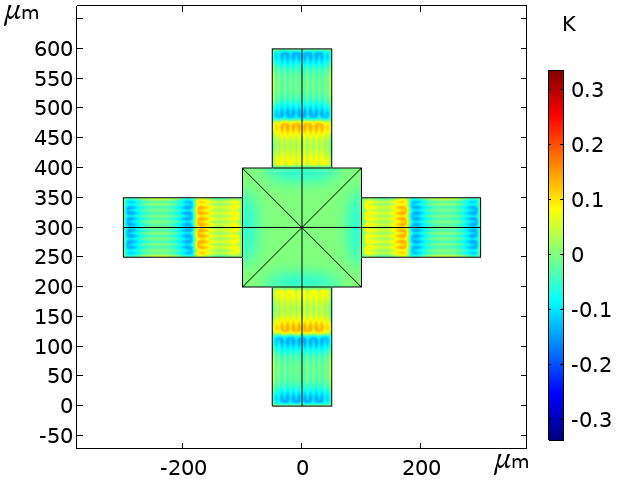
\includegraphics{figures/Simulation/Thermomechanic/AC_temp_field1.png}} &
        \resizebox{0.55\linewidth}{!}{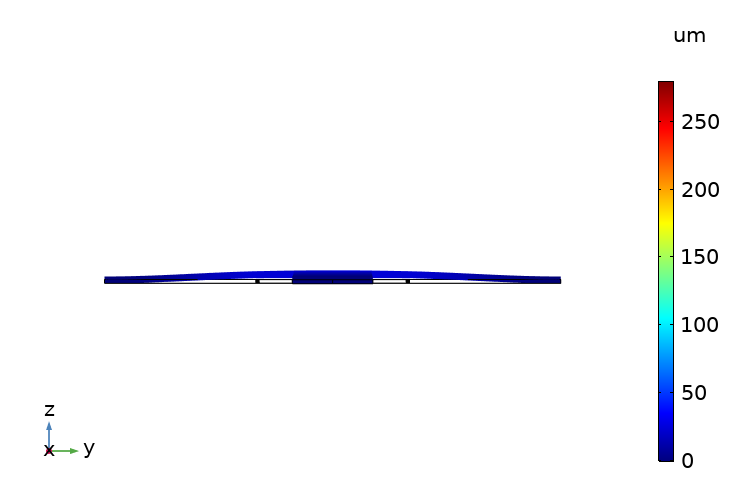
\includegraphics{figures/Simulation/Thermomechanic/Displacement_side1.png}} \\
        \resizebox{0.42\linewidth}{!}{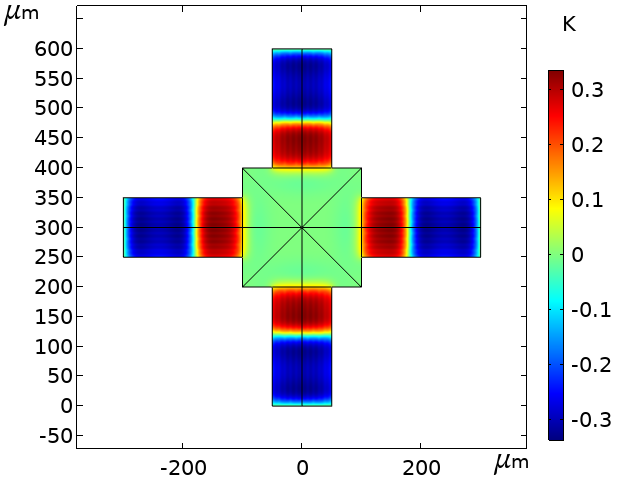
\includegraphics{figures/Simulation/Thermomechanic/AC_temp_field2.png}} &
        \resizebox{0.55\linewidth}{!}{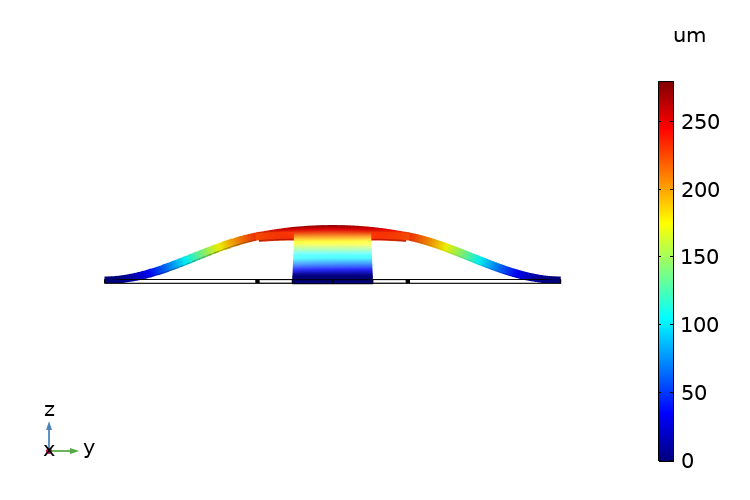
\includegraphics{figures/Simulation/Thermomechanic/Displacement_side2.png}} \\
        \resizebox{0.42\linewidth}{!}{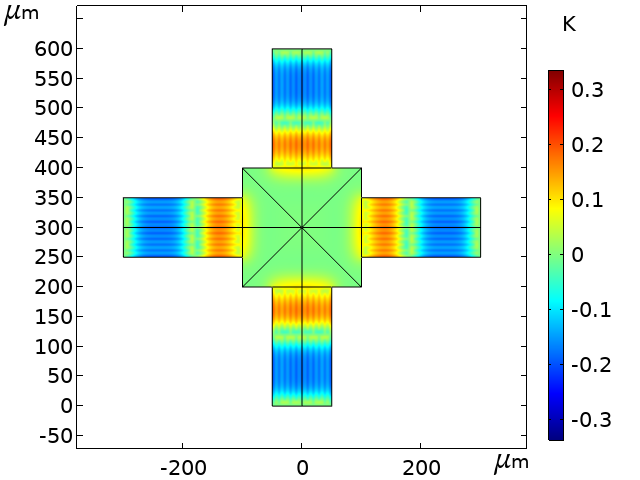
\includegraphics{figures/Simulation/Thermomechanic/AC_temp_field3.png}} &
        \resizebox{0.55\linewidth}{!}{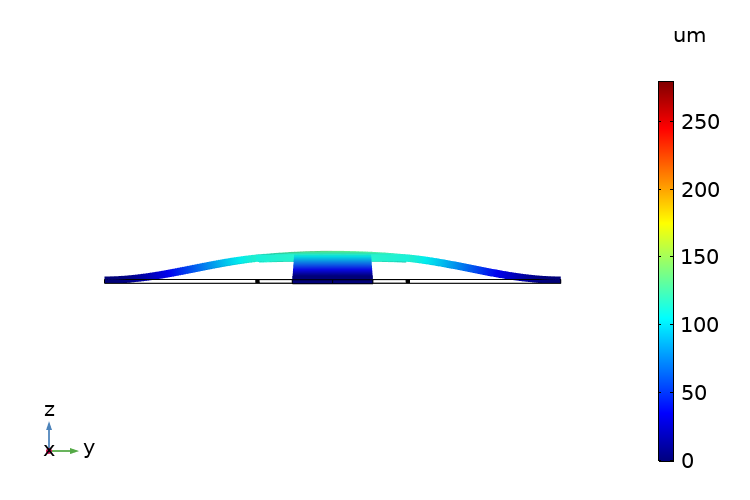
\includegraphics{figures/Simulation/Thermomechanic/Displacement_side3.png}} \\
        \resizebox{0.42\linewidth}{!}{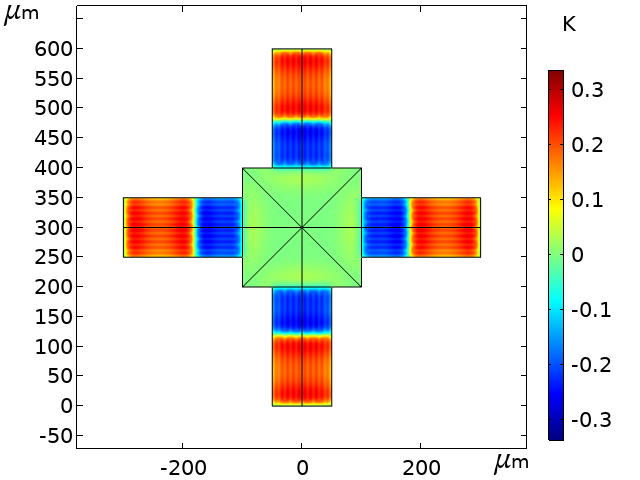
\includegraphics{figures/Simulation/Thermomechanic/AC_temp_field4.png}} &
        \resizebox{0.55\linewidth}{!}{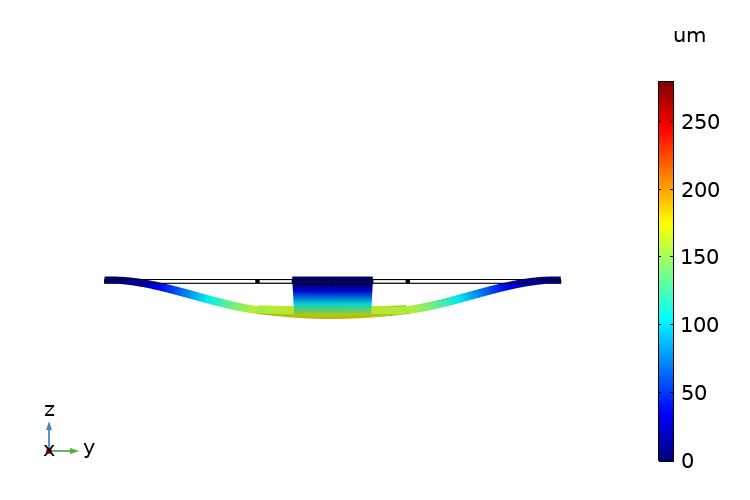
\includegraphics{figures/Simulation/Thermomechanic/Displacement_side4.png}} \\
    \end{tabular}
    \caption{A nagyfrekvenciás hőtágulás okozta rezgés különböző fázisai}
    \label{fig:AC_vibration}
    \vfill
\end{figure}


\subsubsection{Piezorezisztív hatások}

A termomechanikus viselkedés vizsgálata érdekében a mérőfej mozgását a termikus gerjesztést megvalósító ellenállások segítségével vissza is tudjuk mérni kihasználva a piezorezisztív hatást. A mérés elvégzéséhez ismerni kell a mérőfej ellenállás-kitérés karakterisztikáit amikből visszaszámolható a Z irányú kitérés értéke. Ezeknek a karakterisztikáknak a meghatározását a COMSOL Multiphysics beépített piezorezisztív csatolásának segítségével határoztam meg. A szimulációk során a mechanikai rendszernek előírtam a Z irányú kitérését és ebből meghatároztam a karok felületén kialakuló mechanikai feszültségek állapotait. Ezeket az eredményeket felhasználva meghatározható a termikus gerjesztést megvalósító ellenállások mechanikai feszültséggel terhelt ellenállása. Ezeket a karakterisztikákat \aref{fig:piezores_1}. és \aref{fig:piezores_2}. ábrákon mutatom be.

\imgsrclr{figures/Simulation/Thermomechanic/Piezo_1.png}{figures/Simulation/Thermomechanic/Piezo_2.png}{Az 1X mérőfej ellenállásainak ellenállás-kitérés karakterisztikái}{Az 4X mérőfej ellenállásainak ellenállás-kitérés karakterisztikái}{fig:piezores_1}{fig:piezores_2}{1}{1}

A szimulációk során lineáris piezorezisztív hatást és lineáris mechanikai összefüggéseket használtam fel, így a kiadódó karakterisztikák egyenesnek adódtak, ahogy azt el is várhatjuk. Ha a szimulációk során a Green-Lagrange-féle alakváltozási tenzorokat használom fel a mechanikai deformációjára, akkor a kiadódó karakterisztikák parabolikusak lesznek, ahogy azt a másodfokú mechanikai egyenletekből és a lineáris piezorezisztív hatásból várnánk.

A kiadódó karakterisztikák jól tükrözik a két ellenállás alatt kialakuló ellentétes mechanikai feszültségállapotokat, hiszen a kitérés folyamatos növelésével az R1-es ellenállás értéke növekszik, indikálva ezzel a növekvő nyomófeszültség\footnote{A szilárdságtanban a szakító feszültségek előjele pozitív és a nyomófeszültségé negatív, így a negatív piezorezisztív együtthatóval együtt egy pozitív együtthatót adnak.} értéket valamint az N adalékolású szilícium negatív piezorezisztív együtthatóját\cite{piezoresistivity}. Az R2 ellenállásnál a szakítófeszültségek növekednek, így az ellenállás karakterisztikája csökkenő tendenciát mutat.

\subsubsection{Tranziens verifikáció}

A mérőfej tervezésének végső fázisa a megtervezett mérőfej verifikációja. Erre a lépésre azért van szükség, mert a tervezés korábbi stádiumaiban több közelítéssel és elhanyagolással is éltem. Ezek között szerepel például a hőtranszport egyenletben elhanyagolt advektív tag. A verifikáció elvégzéséhez összeállítottam a geometriát és hozzáadtam a COMSOL által biztosított mechanikai és hőtranszport modult. Ezután elvégeztem egy stacionárius szimulációt, a DC komponensek meghatározásához. Ezzel a lépéssel a tranziens szimulációhoz megadhatom az így kiszámolt értékeket, mint kiindulási érték, ezáltal csökkentve a tranziens szimuláció számításigényét, hiszen nem kell megvárni míg beáll az állandósult állapot.

Ezután következett a csatolt fizikai tranziens szimuláció, mely során az állandósult DC állapotból kiindulva időtartományban szimuláltam a mérőfejet. A szimuláció kezdeti szakaszában látható a rezonancia jelensége, hiszen a kitérés amplitúdója az idővel lineárisan növekszik, ahogy az \aref{fig:trans_small}. ábrán látható is. A szimuláció későbbi szakaszában a nemlineáris jelenségek miatt megjelentek a felharmonikusok is a megoldásban, melyet \aref{fig:trans_large}. ábrán láthatunk az amplitúdó modulációjából. Végül a teljes berezgés kitérés-idő diagramját \aref{fig:trans_full}. ábrán láthatjuk. Az ábráról jól látható, hogy a mérőfej kitérései kb. 10 $\mu m$-es nagyságrendnél állandósulnak.

\imgsrc{figures/Simulation/Thermomechanic/transient_full.png}{Tranziens verifikációs szimuláció}{fig:trans_full}{0.8}
\imgsrclr{figures/Simulation/Thermomechanic/transient_small.png}{figures/Simulation/Thermomechanic/transient_large.png}{Kezdeti rezgések lineárisan változó amplitúdói}{Amplitúdó moduláció a felharmonikusok miatt}{fig:trans_small}{fig:trans_large}{0.75}{0.75}

\subsection{Mérőfejváltozatok összehasonlítása}

A megtervezett mérőfejek geometriai adatait és fontosabb szimulációs adatokat \aref{tab:compare}. táblázatban összegeztem. A méretezés során az elektrosztatikus szimulációk eredményéül előálló 50 $\mu m$-es elektródaméretet vettem alapul. Ennek következtében a mérőfejből két különböző változatot készítettem el és szimuláltam le. A két változat között a rezgetett platform mérete az elsődleges megkülönböztető paraméter. Az első változat geometriai mérete 1 mérőelektróda elhelyezését teszi lehetővé, míg a második változatra 4 mérőelektróda helyezhető el egy 2x2-es rácsban. Ebből a parametrikus különbségből származtattam a változatok megnevezéseit is (1X és 4X-es változat).

A platformok méretének különbségéből adódóan a többi geometriai paraméter értékét is csökkentettem, hogy a két változat geometriája egymáshoz hasonló legyen, ezzel megkönnyítve az összehasonlításukat. A kisebb geometriai méretek következtében a rezonanciafrekvenciák is eltolódtak, így a rezonancián létrejövő nagyfrekvenciás hőterjedés is összehasonlíthatóvá vált.

A mérőfejekhez használt bimorf struktúra paramétereit a felhasználni kívánt CMOS gyártástechnológiához igazítottam, ahogy azt \aref{chap:manufacturing}. fejezetben majd láthatjuk. A mérőfejek felületén kialakított ellenállások szélességét és értékét a mérőfejek összehasonlíthatósága érdekében egymáshoz hasonló értéktartományba állítottam be, figyelembe véve a felhasználni kívánt CMOS technológián használható tranzisztorok feszültségszintjeit, így megmaradva a 10-15 V-os nagyságrendnél.

\renewcommand{\arraystretch}{1.2}
\begin{table}[!ht]
    \centering
    \begin{tabular}{@{}llcc@{}}
        \toprule
        & \textbf{Paraméter} & \textbf{Értéke} & \textbf{Mértékegysége} \\
        \hline
        Alapszelet & Adalékolás (bór) & 1 $10^{15}$ & 1/$ cm^3 $ \\
        Leválasztás & Szilárd oldékonyság (foszfor) & 3 $10^{20}$ & 1/$cm^3$ \\
        & Időtartam & 2,5 & óra \\
        & Hőmérséklet & 1000 & $^\circ C$ \\
        Behajtás & Időtartam & 1,5 & óra \\
        & Hőmérséklet & 1100 & $^\circ C$ \\
        Végeredmény & Diffúziós mélység & 2,84 & $\mu m$ \\
        & Elektromos vezetőképesség & 244,32 & S/cm \\
        & Négyzetes ellenállás & 14,4 & $\Omega$/$\square$ \\
        \bottomrule
    \end{tabular}
    \caption{A diffúziós ellenállások számításához használt paraméterek és eredmények}
    \label{tab:diffusion}
\end{table}

A diffúziós ellenállások vezetőképességének számításához az Illinois Egyetem online kalkulátorát használtam fel\cite{Illinois_diffusion}. A kalkulátor paramétereit a Tanszéken található Félvezetőtechnológia Laboratóriumban rendelkezésre álló kályha és az általunk megvalósítható lépéssorozatokat figyelembe véve állítottam. A paraméterek meghatározásánál a felhasználni kívánt CMOS technológián rendelkezésre álló négyzetes ellenállásokat is figyelembe vettem, és igyekeztem a diffúziós ellenállások négyzetes ellenállását is hasonló nagyságrendben megvalósítani. A végleges paramétereket \aref{tab:diffusion}. táblázatban összegeztem.

\begin{table}[!ht]
    \centering
    \begin{tabular}{@{}lccc@{}}
        \toprule
        \textbf{Paraméter megnevezése} & \textbf{1X} & \textbf{4X} & \textbf{Mértékegység} \\
        \hline
        Platformot tartó karok hossza & 200 & 300 & $\mu m$ \\
        Platformot tartó karok szélessége & 100 & 150 & $\mu m$ \\
        Platform szélessége & 200 & 400 & $\mu m$ \\
        Szilícium hordozó vastagsága & \multicolumn{2}{c}{5} & $\mu m$ \\
        Réz bevonat vastagsága & \multicolumn{2}{c}{4} & $\mu m$ \\
        Első rezonanciafrekvencia & 151,54 & 52,63 & kHz \\
        Ellenállások szélessége & 5,6 & 9,75 & $\mu m$ \\
        Ellenállások elektromos vezetőképessége & \multicolumn{2}{c}{244,32} & S/cm \\
        Diffúziós ellenállások vastagsága & \multicolumn{2}{c}{2,84} & $\mu m$ \\
        R1-es ellenállás nominális értéke & 2826,7 & 1921,8 & $\Omega$ \\
        R2-es ellenállás nominális értéke & 1826,2 & 1232,3 & $\Omega$ \\
        $\Pi_{11}$-es piezorezisztív együttható & \multicolumn{2}{c}{-0,337} & $\Omega m$/GPa\\
        $\Pi_{12}$-es piezorezisztív együttható & \multicolumn{2}{c}{0,175} & $\Omega m$/GPa \\
        $\Pi_{44}$-es piezorezisztív együttható & \multicolumn{2}{c}{-0,046} & $\Omega m$/GPa \\
        Elért maximális nagyfrekvenciás hőtágulás $\phantom{abc}$ & 250 & 350 & $\mu m$ \\
        \bottomrule
    \end{tabular}
    \caption{A mérőfejváltozatok legfontosabb paraméterei és szimulációs eredményei}
    \label{tab:compare}
\end{table}

A mérőfejek különböző változatainak összehasonlításából látható, hogy az 1X-es mérőfej kb. háromszoros rezonanciafrekvenciával rendelkezik, így a letapogatáshoz szükséges idő háromszor rövidebb, mint a 4X-es változat esetében, ez nem ellensúlyozza a 4X-es változat négy párhuzamos mérését. A 4X-es mérőfej emellett kisebb ellenállásértékek mellett ér el nagyobb kitéréseket, így kisebb feszültségszintek mellett lehet nagyobb teljesítménnyel gerjeszteni a termomechanikus beavatkozót, ami könnyebben megvalósítható a választott CMOS technológiával. A 4X-es változat esetében a kisebb rezonáns frekvencia miatt a nagyfrekvenciás termikus behatolási mélység is nagyobb, így az adott hőteljesítmény nagyobb hőmérséklet változást képes elérni. A méréstechnikai áramkörök kialakításának is a nagyobb mérőfej kedvez jobban, hiszen a rezgetett platformon összességében nagyobb terület áll rendelkezésre analóg áramkörök megvalósítására.

Összességében ezen hatásokat figyelembe véve a 4X-es mérőfej megvalósítása tűnik ígéretesebbnek.

\chapter{Gyártástechnológia koncepció}
\label{chap:manufacturing}

Az előző fejezetekben bemutatott szimulációs és méretezési lépések végeztével előállt a mérőfej végleges terve. A mérőfej gyártástechnológiai tervezése során az elsődleges szempont a Tanszéken található Félvezetőtechnológia Laboratóriumban történő stabil és megbízható gyárthatóság volt. Mivel CMOS gyártósor nem található a laboratóriumban, így a mérőfej áramköri részeit nem tudjuk saját magunk legyártani. Ezeket a részeket ki kell szervezni egy külső cégnek, melyek az áramköri tervek alapján le tudják gyártani az eszközt. Az áramkör legyártását követően a mérőfej egy chip formájában áll elő, hogy ebből a chip-ből előállítsuk a végleges MEMS eszközt, úgynevezett Post-CMOS technológiai lépéseket kell végezzünk a chipen.

A Tanszék számára elérhető gyártástechnológiák közül elsősorban a Circuits Multi-Projects\cite{CMP} (vagy röviden CMP) által kínált technológiákból válogattam. A megtervezett struktúra által támasztott követelményeknek megfelelően a gyártási eljárások közül a Silicon On Insulator (vagyis SOI) szeleteken megvalósított technológiákat létesítettem előnyben. Ezen eljárások közös tulajdonsága, hogy az aktív, áramköri elemeket megvalósító rétegek alatt egy szilícium-dioxidból álló eltemetett réteg található közel a szelet felületéhez. Ez az eltemetett réteg természetes marásgátló rétegként használható a szelet elvékonyítása során. A technológiák közül szintén előnyben részesítettem a vastag fémrétegeket alkalmazókat, ezzel megvalósítva a karok felületén a bimorf struktúrát.

A CMP által biztosított gyártástechnológiák közül a STMICROELECTRONICS 130 nm-es H9SOI-FEM\cite{H9SOI-FEM} eljárása tűnt a legjobb választásnak. A kiválasztott gyártástechnológia alapvetően rádiófrekvenciás áramkörök végpontjaihoz (RF Front End of Line) lett optimalizálva, azonban ez a lépéssor rendelkezett a számomra legkedvezőbb tulajdonságokkal. A gyártástechnológián előállíthatók a szokványos CMOS áramköri elemek, ilyenek a kis- és nagyfeszültségű N- és PMOS tranzisztorok, a sziliciddel adalékolt poliszilícium ellenállások, lineáris MIM (Metal Insulator Metal), MOM (Metal Oxid Metal) és nemlineáris MOS kapacitások, az ESD védelmet ellátó diódák valamint nagy jósági tényezővel rendelkező induktivitások. A gyártástechnológia által szolgáltatott tranzisztorok elsősorban a 2,5 V-os tartományra lettek méretezve, de található 1,2 V-os nagy sebességű és 8-13 V-os nagyfeszültségű tranzisztor is a technológiai könyvtárban. A gyártástechnológián használható sziliciddel adalékolt ellenállások négyzetes ellenállása 10 $\Omega / \square$ és 320 $\Omega / \square$, ezen értékek alapján állítottam be az általam számolt diffúziós ellenállások értékét is, hogy az ellenállások által foglalt területet is jól közelítse a modellem. A kiválasztott gyártástechnológia másik nagy előnye, hogy a rendelkezésre álló négy fémréteg közül a harmadik egy 4 $\mu m$ vastag réz, így a bimorf struktúra is megvalósítható az integrált áramkör gyártása során. Ennek a rétegnek a vastagsága alapján határoztam meg a modellben beállított rézréteg vastagságát.

Ezt a gyártástechnológiát felhasználva a MEMS eszköz áramköri része szokványos analóg integrált áramköri tervezéssel tervezhető. Ezt követően a megrendelt és legyártott chip-et különböző alacsony hőmérsékletű lépésekkel és marásokkal kialakítjuk a chipet körülvevő szilíciumból a MEMS eszköz számára fontos részeket. A pontos lépéssor meghatározásához szükségünk volt a gyártó által szolgáltatott dokumentációra, azonban ezeket még nem kaptuk meg, így a pontos gyártási lépéssor megtervezése nem volt lehetséges.

A végleges gyártási lépéssort nélkülözve inkább egy egyszerűsített változat elkészítését vázolom fel. Ennek az egyszerűsített változatnak a célja a mérőfej mozgatását megvalósító termomechanikus csatolás vizsgálata. Ennek következtében a kapacitív mérés pontossága csak másodlagos prioritást élvezett. Ezen gondolat mellett megtervezett mérőfej csak a diffúziós ellenállásokat és a réz réteget tartalmazza, mely a mérőfej egész felület fogja borítani. A Kelvin-szondás mérés így ugyan elvégezhető, azonban a rendszer felbontóképessége csak korlátozott lesz és nélkülözni fogja a fókuszáló elektróda hatását. Az egyszerűsített változat gyártási lépéseit igyekeztem a végleges chipet tartalmazó lépéssorhoz igazítani, azonban ez csak korlátozottan volt lehetséges a szükséges dokumentáció hiánya miatt. Az így kialakított gyártási lépéseket \aref{fig:manufacturing}. ábrán szemléltetem.

\Aref{fig:manufacturing}. ábrán a lépések jobb megértése érdekében két keresztmetszeti vetületet is ábrázolok. Ezek az AA' és BB' vetületek melyek a chip középvonala mentén függőlegesen és az egyik kart merőlegesen metszve haladnak. Kiindulásként a SOI szelet felülnézeti képét és a keresztmetszetet ábrázoltam (0. állapot).

Első lépésként a szelet felületén termikus oxidot növesztünk, mely az N diffúzió maszkolását fogja elvégezni. A növesztett oxidot fényérzékeny lakkal vonjuk be, majd ezt UV fénnyel levilágítjuk és kálium-hidroxidos oldatban előhívjuk. Az így előállított és maszkolt oxidot hidrogén-fluoridos oldatba mártjuk, mely eltávolítja a szelet felületén növesztett oxidot ahol azt nem védi a fényérzékeny lakk. Ezt követően eltávolítjuk a fényérzékeny lakkot tömény kálium-hidroxidos oldatba mártva a szeletet. Végül megtisztítjuk a szelet felületét a szerves maradványoktól. Az ebben a paragrafusban leírtakat a gyártás során többször fogjuk megismételni, így a későbbiekben csak litográfia lépésekként fogok erre hivatkozni.

A litográfia lépések után a szelet felületén kialakítjuk a termikus gerjesztést biztosító ellenállásokat egy kétlépcsős diffúziót használva (1. állapot). A diffúzió első lépéseként a szelet felületére leválasztjuk a megfelelő mennyiségű adalékatomot, majd a második lépésben a leválasztott atomokat behajtjuk a kristályrács mélyebb rétegeibe. A diffúzió pontos paramétereit \aref{tab:diffusion}. táblázatban megtalálhatjuk.

A következő lépésben a leírt litográfiai folyamattal kialakítjuk a következő maszkréteget. A szeletet ezután 80 $^\circ C$-s 22 $\%$-os (4 M) kálium-hidroxid oldatban maratjuk\cite{KOH_etch}, míg a karok melletti L alakú területeken el nem érünk az eltemetett oxidrétegig (2. állapot).

A szeletet ezután megtisztítjuk és teljes felületén termikus oxidot növesztünk. A növesztett oxidréteget elektromos szigetelőnek használjuk fel, hogy az erősen adalékolt diffúziós ellenállásokat elszigeteljük a felületi réz rétegtől. A bimorf struktúra kialakításához a mérőfej felületén fényérzékeny lakkal egy maszkréteget viszünk fel, melyen a szükséges területeken ablakokat nyitunk. Az így kialakított maszkon keresztül vákuumpárologtatással és galvanizálással 4 $\mu m$ vastag rézréteget növesztünk, majd eltávolítjuk a fényérzékeny lakkot (3. állapot).

Ezeket a lépéseket követően előáll az egyszerűsített mérőfej rétegszerkezete és csak a szilícium szelet többi részétől kell azt eltávolítani. Azért, hogy megvédjük a rétegszerkezetet a kálium-hidroxidos marástól, a szelet felületén CVD (Chemical Vapor Deposition) eljárással szilícium-nitridet viszünk fel (4. állapot). Ehhez a rétegfelvitelhez a tanszéki laboratóriumban nem áll rendelkezésre a szükséges eszközpark, így ezt a folyamatot az Energiatudományi Kutatóközpont Műszaki, Fizikai és Anyagtudományi Kutató Intézetének a segítségével végezzük el. Ennek a lépésnek egy alternatívája, mely általunk is elkészíthető, a spin-on oxid használata, melyet a fényérzékeny lakkhoz hasonlóan tudunk felvinni a felületre.

Az integrált áramköri gyártótól kapott tokozatlan chipünk rendelkezni fog az összes szükséges réteggel a chip vertikális keresztmetszete mentén, valamint egy passziválóréteggel, mellyel a felső rétegeket védik. Az  chip felületén litográfiával ablakokat nyitunk a kimarandó részeknek, ilyen a hátoldali vékonyítás valamint a 2. lépésnél kialakított karok elválasztása a tömbi szilíciumtól. Ezen ablaknyitások után a chip beültethető az eddig leírt gyártástechnológiába a 4. állapot után.

A szilícium-nitrid által nem védett területeket a már említett 22 $\%$-os oldattal lemarjuk az eltemetett oxidrétegig (5. állapot).

A mérőfej gyártásának utolsó lépése az eltemetett oxidréteg kémiai marása, melyet hidrogén-fluoridos oldattal tehetünk meg (6. állapot).

\imgsrc{figures/Production/manufacturing.png}{Az egyszerűsített mérőfej gyártási lépései}{fig:manufacturing}{0.65}

\chapter{Összefoglalás}

Az elkészített diplomatervem során elmélyedtem a Kelvin-szondás mérés részleteiben és kidolgoztam egy szimulációs tervet a Kelvin-szondás mérőfej elektrosztatikus paramétereinek számítására, valamint az ebből levezetett koncentrált paraméterű modell paraméterezésére. A szimulációs folyamatot jelentősen megkönnyítő automatizálás lehetőségét kihasználva, elmélyedtem a COMSOL Multiphysics által biztosított LiveLink környezetében és ennek eredményéül jelentős mértékben sikerült a szimulációkat meggyorsítani, valamint az utófeldolgozást elvégezni. A vizsgált konfigurációk elektrosztatikus paramétereinek meghatározása után lehetőség nyílt a konfigurációk között választani és a további tervezési feladatokat specifikálni.

Az elektrosztatikus szimulációk eredménye alapján a mérőfej mechanikai specifikációja is előállt. Ezen specifikációknak megfelelően megterveztem a Kelvin-szonda rezgő elektródáját meghajtó MEMS eszköz két különböző változatát melyek közelítően megfelelnek az általam támasztott specifikációknak. A megtervezett és méretezett eszközön végül egy termomechanikus szimulációval meggyőződtem annak működőképességéről. Elkészítettem egy numerikus szimulációt PYTHON programozási nyelvben, mely figyelembe veszi a mérőfej elektrosztatikus és termomechanikus karakterisztikáit a mérőfejen mérhető feszültségjel számítására. Felvázoltam egy lehetséges architektúrát a mérőfej jelének mérésére CMOS technológián figyelembe véve a termikus zajt. Megvizsgáltam a termikus beavatkozást biztosító ellenállások felhasználhatóságát a mérőfej kitérésének mérésére kihasználva a Piezorezisztív-hatást és elkészítettem az ellenállások megfelelő karakterisztikáit.

Az elektrosztatikus és termomechanikus szimulációk lefuttatását követően megvizsgáltam az általam tervezett mérőfej gyárthatóságát. A gyárthatóság vizsgálatánál egy SOI szeletet felhasználó nagyfrekvenciás áramkörök megvalósítására optimalizált technológiát használtam fel, melyet kiegészítettem a tokozást megelőző, utólagos lépésekkel, melyekkel az áramkör átalakítható egy MEMS eszközzé, a folyamat során megőrizve az eredeti áramköri kapcsolástechnikát a szelet felületén. Elkészítettem a mérőfej egyszerűsített változatához tartozó gyártástechnológiai lépéssort mellyel az egyszerűsített mérőfej a BME Félvezetőtechnológia Laboratóriumában legyártható az Energiatudományi Kutatóközpont Műszaki, Fizikai és Anyagtudományi Kutató Intézetének közreműködésével.

\chapter*{Köszönetnyílvánítás}
\addcontentsline{toc}{chapter}{Köszönetnyílvánítás}

Ezúton szeretnék köszönetet mondani konzulenseimnek Dr. Plesz Balázsnak és Dr. Szabó Péter Gábornak a diplomamunkám elkészítésében mutatott kitartásukért, segítőkészségükért és rugalmasságukért. Szeretném megköszönni Dr. Plesz Balázsnak a gyártástechnológiai tanácsokat, meglátásokat és ötleteket, valamint Dr. Szabó Péter Gábornak a szimulációs eljárások elsajátításában nyújtott segítségét.

Végezetül szeretném megköszönni Családomnak és barátaimnak az általuk nyújtott támogatást és szeretetet amelyek nélkül nem tudtam volna elkészíteni Diplomamunkám.

%----------------------------------------------------------------------------
\appendix\label{appendix}
%----------------------------------------------------------------------------

\chapter*{Függelék}
\addcontentsline{toc}{chapter}{Függelék}
\setcounter{chapter}{\appendixnumber}

A diplomamunkám áttekinthetőségéhez és későbbi újraellenőrzésének érdekében a felhasznált COMSOL, MATLAB és PYTHON fájlokat valamint az összes felhasznált kódot elérhetővé teszem egy \href{https://github.com/Dandubacsi/dipterv}{\color{blue}{github repository}}-n keresztül. 


\listoffigures\addcontentsline{toc}{chapter}{\listfigurename}                   % List of Figures, Tables
\listoftables\addcontentsline{toc}{chapter}{\listtablename}

\printbibliography[title = Irodalomjegyzék]                                     % Bibliography

\end{document}
